\documentclass{xdupgthesis}
\usepackage{listings}
\usepackage[ruled]{algorithm2e}
\usepackage{minted}
\usepackage{booktabs}
\usepackage{multirow}
\usepackage{xspace}
\usepackage{enumitem}
\usepackage{subfig}
\usepackage{tikz}
\usepackage{amsmath}
% \usepackage{cases}
\usepackage{makecell}
\usepackage{threeparttable}
\usepackage{diagbox}
\usepackage{amsfonts}
\usepackage{pifont}

% 标记
\newcommand{\param}[1]{\mbox{\small{\texttt{#1}}}}
\newcommand{\func}[1]{\mbox{\small{\texttt{#1}}}}
\newcommand{\dquote}[1]{“#1”}
\newcommand{\tool}[1]{{\textit{#1}}}

% 特殊工具
\newcommand{\icsearcher}{\textit{ICSearcher}\xspace}
\newcommand{\deccheck}{\textit{DecChecker}\xspace}
\newcommand{\nyctea}{\textit{ICFixer}\xspace}

% 代码
% \renewcommand\listingscaption{代码}

% 流程
\newcommand*{\circled}[1]{\lower.7ex\hbox{\tikz\draw (0pt, 0pt)circle (.5em) node {\makebox[0.5em][c]{\small #1}};}}

\xdusetup{
style / cjk-font = fandol,
style / latin-font = gyre,
style / bib-backend = bibtex,
style / customize-edubg = true,
style / customize-resresult = true,
% 信息
info / title = {基于人工智能的无人机系统可靠性技术研究},
info / title* = {Ensuring Reliable of UAVs system through Artificial Intelligence},
info / author = {韩瑞冬},
info / author* = {Ruidong Han},
info / supervisor = {马卓},
info / supervisor* = {Zhuo Ma},
info / supervisor-title = {教授},
info / supervisor-title* = {Professor},
info / supervisor-enterprise = {西安电子科技大学},
info / supervisor-enterprise* = {Xidian University},
info / degree = {工学博士},
info / graduate-type = {博士},
info / degree-type = {学术},
info / major = {网络空间安全},
info / major* = {Cyber Security},
info / sub-major = {网络空间安全},
info / department = {网络与信息安全学院},
info / student-id = {20151110321},
info / abstract = {tex/abstract.tex},
info / abstract* = {tex/abstract_en.tex},
info / keywords = {无人机系统可靠性, 模糊测试,在线检测,机器学习预测, 深度强化学习},
info / keywords* = {Unmanned aerial systems security, Fuzzy test, Online detection, Machine learning prediction, Deep reinforcement learning},
% 符号表
info / los =  {table/los.tex},
% style/customize-los = false,
% 缩略语
info / loa =  {table/loa.tex},
% 引用
info / bib-resource = {ref.bib},
% 个人简介
info / bio = {tex/bio.tex},
% 致谢
info/acknowledgements = {tex/acknowledgements.tex}
}


\begin{document}

\frontmatter

\mainmatter

\chapter{绪论}
\section{研究背景及意义}
% 无人机的废话
得益于人工智能等许多领域的进步,无人机在我们的日常生活中的应用场景迅速增长。
从军事战术到商业应用,无人机在各个领域展现出了巨大的潜力~\cite{chabot2018trends,banos2020assessment,patino2009adaptive,shukla2016application,huang2021multi,li2018uav}。
例如,新闻报道和电影制作可以通过无人机获取不同的视角和高质量的影像,极大地丰富了视觉效果。
在地理测绘方面,无人机可以到达人类难以抵达的地方,为地理信息系统提供了更多的数据来源~\cite{news1}。
在灾害情况信息收集方面,无人机可以在灾难发生后迅速进入现场,为救援团队提供准确的现场信息~\cite{news2}。
在人道主义救援行动中,无人机可以通过热传感器寻找被困的人,从而提供及时的救援~\cite{polka2017use}。
此外,亚马逊Prime Air、谷歌Wing、UPS Flight Forward等公司公开宣布了计划从空中运送包裹的快递配送方案~\cite{news3}。
这些公司的无人机配送服务都是在尝试利用无人机技术来提高配送效率、降低配送成本,并尝试为顾客提供更快速的配送服务。
东京奥运会开幕式等活动也以无人机灯光秀为特色。

% 在军事方面,无人机可以执行侦察、打击等任务,降低了士兵面临的风险。
% 在物流领域,无人机可以用于快递送货,加快了货物的运输速度。
% 在科研领域,无人机可以用于大气探测、地质勘探等任务,为科学研究提供了新的工具。
% 在娱乐领域,无人机也被广泛应用于航拍、比赛等活动,为人们带来了全新的娱乐体验。
% 总的来说,其多功能性使其成为一种重要工具,随着技术不断发展和创新,无人机在各个领域的作用将继续扩大。

% 无人机的而可靠性不行
然而,由于无人机轻量化、高实时性、多应用场景的特性,大部分无人机系统(如\tool{Ardupilot}和\tool{PX4})的实现较为初级,缺乏一定的可靠性和功能验证,其造成的系统漏洞在部分场景和条件下会对无人机产生物理损伤。
且由于无人机体系架构碎片化的问题 (例如四旋翼和六旋翼),现有的开发和使用人员难以根据自身飞行任务的需要,准确的配置或修改无人机。
近几年的研究~\cite{wang2021exploratory,choi2020cyber}表明,无人机系统在其设计与实现层面存在较大的问题,容易引入可被利用的系统设计漏洞。
甚至全球最大的商用无人机开发商大疆,也存在旧机型上的系统设计漏洞~\cite{schiller2023drone},且并未被修复。
这些碎片化、多场景、复杂的飞行问题更加剧了无人机系统的设计难度,进而在无人机系统上引入系统可靠性的问题。

% 现有的发现的无人机的问题
这些可靠性问题存在于无人机系统中的不同机制模块当中,都会影响无人机的飞行。
例如,由于系统设计缺乏抗干扰而数据二次验证,无人机传感器模块读数受到干扰或者其融合模块噪声影响时~\cite{daneshmand2012low,gaspar2020capture,huang2015gps},会使得无人机系统错误认知自己所处的飞行环境,进而做出错误的反应,引发飞行失控。
由于缺乏基本的加密和通信验证机制,无人机的通信模块如果受到恶意伪造攻击时,可能会接收错误的命令和消息~\cite{li2018protecting,chen2019machine},同样会导致无人机飞行失控。
更难以察觉的是系统功能设计层面的问题。
功能设计缺陷~\cite{rvfuzzer,han2022control,wang2021exploratory,choi2020cyber,aggarwal2020path}会使无人机中相应的系统影响飞行中的可靠性和稳定性。
在特定环境、配置或任务的情况下,这些影响可能会造成无人机失控,完全脱离使用者的掌控。
同时,由于是系统功能设计所导致,因此此类问题并不容易被开发者提前发现,进而难以定位问题根源,无法及时修复。
此外,如果无人机的使用者缺乏操作经验,也会造成主动触发这些问题,从而\dquote{主动}影响无人机的系统可靠性。


% 现有的解决和仍然存在的问题
相关综述~\cite{derhab2023internet,omolara2023drone}表明,无人机系统中大量影响飞行可靠性的问题
与姿态控制和任务执行相关。
也就是说,一个系统功能与姿态控制和任务执行的联系越紧密,其功能设计上问题越容易导致无人机出现不可挽回的损失。
例如,无人机系统中的数据融合功能影响系统对自身姿态的判断、安全检查功能影响无人机自身的姿态调整、参数配置功能影响无人机的姿态调整和任务适应性、姿态稳定功能则直接影响飞行时无人机的动态调整。
现有大量的研究~\cite{heredia2008sensor,quinonez2020savior,samy2008neural,fei2018cross,dash2021stealthy,sindhwani2020unsupervised,lu2017motor}针对数据融合模块提出了切实可行的可靠性提升方案,有效减少数据对无人机飞行的影响。
然而,无人机其他功能仍面临着较初级的保护。
无人机不一致现象~\cite{choi2020cyber}揭示了其安全检查功的设计缺陷;
参数规范错误~\cite{rvfuzzer,han2022control}则指出了无人机参数配置功能的功能缺陷;
而部分研究~\cite{choi2020software,dash2021pid}直接表明,无人机缺乏最基本的飞行中动态修复保护方案。
也就是说,无人机系统中的部分核心组件仍需要提升其功能的可靠性。
本文需要关注无人系统的特点,通过整合先进的人工智能和机器学习技术,面向上述无人机系统中仍存在的系统问题,研究更加可靠的安全检查、参数配置和在线修复方案,从而实现更加可靠的飞行,最大程度地减少意外事件和损失的发生。


% 近年来的相关安全研究也更加聚焦无人机系统。
% 通过模糊测试~\cite{rvfuzzer,han2022control}、故障定位~\cite{mayday,choi2020cyber,kim2022pgpatch}、异常检测~\cite{heredia2008sensor, crowdgps,lu2017motor}等手段强化无人机系统的方案也日益增多。
% 整体上,无人机安全性和可靠性增强通常从三个角度入手。


% \begin{enumerate}
%     \item \textbf{增强模块功能:} 无人机自身提供了初级的安全模块用于应对飞行中出现的安全问题或不稳定飞行。
%     但是开发者由于缺乏经验,此类模块所提供的功能较为初级,无法覆盖更广的场景。
%     因此,部分研究~\cite{heredia2008sensor,choi2020cyber}通过修改其自身的安全模块来提升无人机的能力。
%     此类研究通过提升无人机应对已有问题的能力来提高安全性和可靠性。

%     \item \textbf{完善系统机制:} 无人机系统设计环节可能存在漏洞。
%     因此部分研究~\cite{rvfuzzer,han2022control}通过算法搜索逻辑漏洞从而修复无人机系统中存在的问题。
%     此类研究通过完善系统机制来提高安全性和可靠性。

%     \item \textbf{增加动态功能:} 无人机本身是一种动态飞行设备,许多问题出现在无人机的飞行过程当中。
%     部分研究~\cite{choi2020software,dash2021pid}通过在无人机上或监测系统中添加额外的功能来及时发现无人机的问题并提供相应的补救措施,从而在不中断无人机飞行的情况下,修正无人机。
%     此类研究通过提供额外的在线监控和修补功能提高安全性和可靠性。
% \end{enumerate}
% 然而,相关综述~\cite{derhab2023internet,omolara2023drone}表明,现阶段的无人机系统仍会出不可预料安全问题。

% 其无人机的系统的安全性和可靠性仍有加强的空间。
% 因此,本文需要关注无人系统的特点,通过整合先进的技术,丰富无人机安全相关的功能,提升无人机系统自身的安全性和可靠性,保证飞行和任务的正常执行,从而最大程度地减少意外事件和损失的发生。


\section{国内外研究现状}
本节将介绍国内外与无人机系统可靠性相关的研究。
包含数据融合功能中异常数据识别的研究,无人机系统漏洞发掘及修复相关研究,以及有助于系统漏洞发掘的现有工具和方案。


\subsection{无人机异常数据识别}
现有的文献从多角度对无人机上的错误识别和异常检测方法进行了讨论。

\subsubsection{无人机异常数据监控}
基于监测和参数估计的方法是最常用的故障检测方法。 
近年来发表的大多数关于无人机系统的工作也使用基于监测的方法。
监测的方法背后的基本思想是通过在确定性设置中使用观察器来估计系统的输出。
一旦预估与实际发生偏离,则认为是异常。

一些研究用不变量来作为飞行过程中数据的监测器来识别异常。
\citet{choi2018detecting}提出了一种攻击检测框架,通过推导和监控控制不变量 (Control Invariant) 来实时识别针对无人机车辆的外部物理攻击。
该方法通过对车辆的物理特性、其控制算法和物理定律进行联合建模来提取此类不变量的方法。
这些不变量以状态空间形式表示,然后可以实现并插入车辆的控制程序二进制文件以进行运行时不变检查。
一旦飞行值偏离控制不变量所预期的值过大时,该程序认为无人机受到了攻击。
为了检测无人机系统中的故障组件,故障检测方法~\cite{heredia2008sensor} 构建了一个监测器模型,它根据历史输入和输出估计无故障条件下的输出。
它采用输出值与预测值之间的偏差来识别有故障的传感器和执行器组件。
\citet{quinonez2020savior}通过攻击检测算法、反击模型以及在硬件最小性能开销这三个功能的组合,引入了\tool{SAVIOR},一种隐形攻击监测系统,基于物理数据的监测机制为自动驾驶汽车提供安全保障,与控制不变量不同,它们的不变量的设计是参考的转子的转速输出。

其他研究采用冗余数据的方式来构建监测器。
基于神经网络的验证方法~\cite{samy2008neural} 利用飞行参数之间的分析冗余来检测传感器故障。
它在无人机模型上利用飞行参数之间的分析冗余,选择使用扩展最小资源分配网络 (Extended Minimum Resource Allocating Network) 算法在线训练的径向基函数 (Radial-Basis Function) 进行神经网络建模,用生成的模型去检测错误。
\citet{fei2018cross} 设计了一个名为\tool{BlueBox}的框架,通过外部件来监控车辆减少了原始系统的修改。
它从车辆源代码上提取车辆的控制逻辑,并在外部硬件上实现了与控制逻辑相类似的功能从而实现高精度的错误检测。 
结合软件和硬件冗余,\tool{BlueBox}能够检测对传感器、控制器、车辆动力学、执行器和控制器操作系统的各种攻击。

此类数据监控方式从无人机数据变化模式下手,建立数据变化的\dquote{基本规律},以模型的形式预测无人机的正确输出,从而实现检测。

\subsubsection{机器学习异常检测}
在此进一步的基础上,一些方案尝试将数据监控与机器学习内容相结合。
\citet{dash2021stealthy} 展示了基于控制的入侵检测中的漏洞,并提出了三种逃避检测和破坏无人机任务的隐形攻击方法。 
针对这种攻击,该同时提供了执行攻击的自动化算法,无需攻击者花费大量精力或了解飞行设备的具体细节。
\citet{sindhwani2020unsupervised}使用机器学习方法和模型通过对无人机的传感器飞行参数进行训练来生成一种新颖的异常检测框架。
它引入了聚类方法来解决群体飞行中标记数据的缺乏和正常数据与异常数据之间的不平衡问题。
该框架基于学习的数据驱动方法,用于群体飞行中的异常检测。
\citet{lu2017motor} 使用强化学习进行运动异常检测。
他们采用学习模型来预测电机温度的变化趋势,并监控每个动态状态的预测温度偏差。
如果检测到温度异常,无人机将自动降落,如果温度恢复正常,则恢复飞行,这个系统可以防止无人机在极端环境下坠毁。
自动电机异常检测系统提高了安全性,允许更积极地使用自动驾驶,从而减少因通信丢失和控制器错误引起的碰撞。
\citet{ahn2019learning}提出了一种基于学习的数据驱动方法,用于群体飞行中的异常检测。
该方法主要试图解决群体飞行中缺乏标记数据以及正常和异常数据不平衡的问题。
他们首先利用主成分分析首先降低飞行数据时间序列的维数,然后使用K均值聚类将数据分组并将它们标记为四类。 
最终,该方法训练了一个由一维卷积神经网络和多层感知器串联而成的深度神经网络,来提取特征和进行检测异常。
\citet{abbaspour2016detection} 介绍了一种自适应神经网络算法来检测无人机设备中的故障数据注入攻击。
他们使用该网络来检测无人机传感器中的注入故障,其中扩展卡尔曼滤波(Extended Kalman Filter,EKF) 用于在线调整神经网络权重。
这种在线调整使攻击检测更快、更准确。

类似的,本文问题的解决方法将机器学习方法与监测器相结合,实现了比传统线性方案更高的预测准确度。



\subsection{基于学习的模糊测试}
随着机器学习理论的发展,其应用于安全测试的案例也随之增多。
\tool{NEUZZ}~\cite{she2019neuzz}介绍了一种新颖、高效、可扩展的程序平滑技术,该技术使用前馈神经网络,可以逐步学习复杂的、真实世界的程序分支行为的平滑近似,即预测由特定输入行使的目标程序的控制流边缘。
该技术进一步提出了一种梯度引导的搜索策略,计算并利用平滑近似的梯度来确定目标突变的位置,使目标程序中检测到的错误数量最大化。
\citet{kim2021pgfuzz}开发了\tool{PGFUZZ},一种基于策略的模糊测试框架用于验证无人机程序是否遵循定义的安全和功能策略。
\tool{PGFUZZ}包括,预处理,策略引导的模糊测试,和Bug后处理共三个组件。
在预处理组件中,\tool{PGFUZZ}通过度量时间逻辑的表示的策略来表达无人机中的操作逻辑,并通过查找与测试策略相关的输入来最小化模糊测试空间。
然后,策略引导的模糊测试对预处理组件识别的输入进行变异,当全局距离变为负值时,就认为检测到违反策略。
最终,\tool{PGFUZZ}通过错误后处理组件来排除与策略违规无关的输入来最小化触发错误的输入序列。
\tool{ExploitMeter}~\cite{yan2017exploitmeter}提出了一个名为\tool{ExploitMeter}的框架,它使用动态模糊测试和基于机器学习的预测来更新对软件可利用性的判断。
\tool{ExploitMeter}框架的核心是一个模仿人类评估者认知过程的贝叶斯推理引擎:使用其静态特征,评估者首先从基于机器学习的预测中得出它对软件系统可利用性的先验信心,然后通过使用不同的模糊器进行一些动态模糊测试,并通过新观察来更新她对软件可利用性的信念。
总体上说,\tool{ExploitMeter}的推理引擎可以被描述为一个动态非线性系统,其输入为来自基于机器学习的预测和动态模糊测试。

学习引导的模糊测试~\cite{chen2019learning}提出了一种自动化的机器学习引导方法,用于构建工业系统中网络攻击的模糊测试。
该技术使用预测机器学习模型和元启发式搜索来智能地模糊执行器命令,并系统地将系统驱动到不同类别的不安全物理状态。
它首先通过对描述其正常行为的物理数据日志进行机器学习算法训练,学习数据变化模型。
学习到的模型可以用来预测当前的物理状态在不同的执行器配置下会如何演变。
随后,它通过网络对执行器进行模糊测试,从而找到驱动系统进入目标不安全状态的攻击序列。
\citet{bottinger2018deep}研究了如何将模糊测试形式化为学习问题。
对于模糊测试来说,模糊器生成新的输入,然后使用每个输入运行目标程序。 
对于每个程序执行,模糊器提取运行时信息以评估当前输入的质量。
同样,强化学习设置定义了与系统交互的代理。 
每个执行的动作都会导致系统的状态转换。
在执行每个动作后,代理会观察下一个状态并获得奖励。 
两者在工作流程上是相似的,因此该研究最终采用Q-learning~\cite{mnih2013playing}算法来进行模糊测试。
\tool{DeepSmith}~\cite{cummins2018compiler} 提出的是一种快速、有效且省力的方法来生成用于编译器模糊测试的随机程序。
\tool{DeepSmith}使用深度学习来自动构建人类如何编写代码的概率模型,它能够推断出编程语言的语法和语义以及常见的结构和模式。
其方法的本质是将随机程序的生成框定为语言建模问题,这极大的简化了并加速了生成过程。
如此以来,生成程序的表现力仅受语料库中包含的内容的限制,不需要开发人员的专业知识或时间消耗。

上述研究表明,将模糊测试应用于无人机当是发现系统设计问题的切实有效的方法。
且与预测模型的结合行之有效。




\subsection{无人机系统分析与修复}
近年来的研究,通过分析无人机系统中的逻辑问题发现了许多漏洞。
从软件设计的角度来看,无人机程序存在一些系统缺陷,可能导致不可预测的结果或在攻击无人机时被利用。
~\citet{wang2021exploratory} 通过调查无人机错误报告、源代码、补丁和历史数据,并对两个主要的无人机开源自动驾驶软件平台,分析了无人机特定错误和相关根本原因,总结了常见的错误模式和修复策略。
\citet{liang2021understanding}进行了一项实证研究,以从自下而上的现场开发人员的角度理解软件的安全关键问题。
他们专注于控制软件中边界函数(Boundary Function)的运行时检查,使用静态方法对边界函数实例进行分类,并通过差异方法动态评估边界函数使用的影响。
\tool{RVFuzzer}~\cite{rvfuzzer}探讨了无人机控制程序中的一种新型漏洞,它涉及对控制参数输入的缺失或不正确的验证检查。
它通过控制引导的输入突变查找无人机控制程序中的输入验证错误。
\tool{RVFuzzer}涉及一个控制不稳定性检测器,该检测器通过基于控制模型观察(模拟)无人机的物理操作来检测控制程序的不当行为。 
此外,它还通过利用控制不稳定性检测器的结果作为反馈,引导输入生成以更有效地查找输入验证错误。
\citet{choi2020cyber} 提出了一种新的基于测试的网络物理不一致(Cyber-Physical Inconsistencies)性检测技术。
该程序分析并提取无人机关于状态或传感器的安全检测模块的谓词条件。
它对该谓词条件进行测试,并通过虚拟车辆和物理测试车辆的差异化状态来测试出无人机运行时物理状态和网络空间不一致的漏洞。
这种的漏洞可能导致安全检查无法报告真实的物理事故或误报。

此外,针对无人机出现安全问题或者系统问题后的修复方式,以下方案也进行了探讨。
随着无人机的广泛采用,它们的事故越来越多,需要对此类事故进行深入调查。
\tool{MAYDAY}~\cite{mayday}认为当前无人机的飞行日志仅记录高级车辆控制状态和事件,不记录控制程序执行。
这使得控制器异常到程序错误定位之间缺乏有效的追踪。
而\tool{MAYDAY},旨在通过将控制模型映射到控制程序来实现无人机事故的跨域调查。
它分析控制和程序级日志从而追踪导致事故的控制语义错误,给出无人机事故的错误原因。
\citet{choi2020software}为多传感器载具提出了一种新的软件传感器恢复技术以抵御物理传感器的攻击。
该方法采用所谓的软件传感器作为相应物理传感器的备份,它可以在同类或不同类的多个传感器受到攻击时恢复。
此方法是纯粹基于软件的,不需要任何额外的硬件。
在运行过程中,软件传感器不断计算和预测相应物理传感器的读数。
当检测到某些物理传感器受到攻击时,相应的软件传感器可以隔离和替换被攻击的传感器,并从损坏的内部状态中恢复系统,以防止严重的攻击后果(例如,崩溃和物理损坏)。
与上述方法类似,\tool{PID-Piper}~\cite{dash2021pid}是一个通过使用辅助控制器与无人机的主控制器串联来实现运行时恢复的框架。
不同于\tool{MAYDAY},\tool{PID-Piper}用前馈控制器,而不是后馈控制器。
使用前馈控制器可以有效避免避免控制器的过度补偿问题。
其次,\tool{PID-Piper}使用机器学习来学习预测控制器输出的模型,并使用特征工程来避免模型的高共线性问题。
\tool{PGPATCH}~\cite{kim2022pgpatch} 为无人机车辆控制程序提出了一个策略引导的程序修复框架,它可以为给定的逻辑错误生成补丁并在没有人为干预的情况下应用它们。
\tool{PGPATCH}由四个相互关联的组件组成:(1) 预处理器,(2) 补丁类型分析器,(3) 补丁生成器,以及 (4) 补丁验证器。
\tool{PGPATCH}首先使用预处理器接受一个触发错误的输入,然后通过补丁类型分析器找到最合适的补丁类型来修复特定的逻辑错误,进而通过补丁生成器组件为目标错误找到合适的补丁位置,并创建一个补丁,最终通过补丁验证器确认该补丁没有破坏无人机的功能或降低其性能。




\section{研究内容}
为了实现无人机系统可靠性,本文从无人机系统本身出发,针对上述无人机系统中仍存在的系统问题,研究更加可靠的安全检查、参数配置和在线修复方案。
具体研究内容如下:
\begin{itemize}
    \item \textbf{不变量验证的可靠安全检查方案:} 
    由于传统的安全检查模块在处理复杂不安全事件上能力有限,所以本文提出了一种新的可靠安全检查方案。
    通过深度学习模型引入不变量异常检测系统,其核心是生成了一种状态不变量,这是一种特殊的预测器,能够描述未来的飞行状态变化。
    系统结合预测偏离检测的方式生成对当前飞行的状态描述。
    然后,该模块使用基于机器学习的检测器来识别是否发生了复杂事件,并制定出相应的应对策略。
    这种新的安全检查模块能够识别出无人机自身系统检查未能检测到的遗漏事件,并减少由于原先检测系统过于敏感而产生的误报。

    
    \item \textbf{模型预测的可靠参数配置方案:} 
    由于无人机系统面临范围规范错误问题, 本文提出一种模型预测的可靠参数配置方案。
    该方案针对无人机系统参数配置机制中的范围规范错误问题,使用预测引导模糊测试的思路,识别出可能引发错误的配置或不合适的参数组合,并对这些参数提出更合理的范围。
    为了更精确地找到可能导致无人机出现范围规范错误的配置,该方案采用了元启发式搜索算法。
    而且,为了提高配置评估的速度,该方案还引入了基于机器学习的预测器。
    这种方法能有效降低模糊测试中的执行验证次数,从而大大提升了搜索的效率。
    其能有效减少参数配置对于无人机系统可靠性的影响。
    
    
    \item \textbf{强化学习的可靠在线修复方案:} 
    针对无人机姿态稳定算法无法应对不正确配置的影响(攻击或自身设置错误),本文提出一种强化学习的可靠在线修复方案。
    该方案的核心是通过观察偏差数据,即实际飞行状态与预期飞行状态之间的差距,来预测潜在的不稳定状态。一旦预测到不稳定状态,该方案会在无人机失控前对其进行纠正。
    在纠正不稳定状态时,该方案会调用预先通过强化学习训练的智能代理,自动生成适当的修正,然后重新配置无人机以避免进入失控状态。
    这种修正过程是迭代进行的,直到不稳定性被消除。
    其能有效减少在线飞行时受到攻击而对系统可靠性产生影响。
    
\end{itemize}

% 本文的主要贡献如下所示:
% \begin{enumerate}
%     \item 本文提出一个用于安全检查模块的辅助模块,\deccheck。 
%     其为不安全事件创建特征描述,并利用检测器识别这些事件,同时提供适当的建议。
%     具体来说,受不变性属性的启发,本文设计一种为无人机提取状态不变的新方法。
%     不变量可以估计未来的飞行状态,并为复杂的不安全事件创建更精确的特征描述。
%     \deccheck 通过结合这些特征与一个神经网络分类器,识别飞行中出现检测模块的错误汇报。
%     提高了无人机自身检查模块的可靠性,降低潜在不安全事件对于无人机的影响。
    
%     \item 本文提出一种模糊测试模块结合预测器来寻找不正确的配置并提供指导,\icsearcher。 
%     \icsearcher 依赖于遗传算法(GA)和飞行状态预测器来检测潜在的不正确配置。
%     它利用过往的飞行经验来生成一个预测器,用于在模糊测试过程中评估潜在不正确配置。
%      同时,\icsearcher 使用段偏差数据来量化配置的效果,以减轻瞬态偏差或噪声的影响。
%      为了平衡开发人员要求的可靠性和适应性,\icsearcher 系统利用优化方法来提供多种灵活的范围指南,以最大限度地减少包括错误配置的可能性,同时保持广泛的范围空间。
%      提高了无人机在使用过程中的可靠性,保障用户在使用过程中的安全性。

%     \item 本文提出一种飞行状态矫正模块,\nyctea。
%     \nyctea 结合配置设置和强化学习的特点来构造一个自适应的智能代理。
%     通过综合探索各个飞控程序中配置与对应飞行状态之间的相关性,代理可以根据物理飞行状态和当前操作要求生成适当的配置。
%     \nyctea 建立在大多数飞行控制程序支持的配置设置方案之上,它可以很容易地与现有的飞行控制程序集成。
%     \nyctea 搞笑准确的解决了无人机飞行过程中的动态校准问题,在发现异常的同时,能够在不中断任务的情况下有效的提高无人机飞行的可靠性。
    
% \end{enumerate}
  
\section{本文组织结构}
本文主要研究面向无人机的安全性和可靠性强化方法。
全文分为六个章节,各章节内容如下:

\textbf{第一章}为绪论,
\textbf{第二章}为预备知识,对本文后续用到的关键技术进行介绍。
\textbf{第三章}对于无人机安全检查模块中的存在的检查不充分的情况进行了分析。有针对性的设立了辅助检测工具用于发现这类检查不充分的情况和场景,并提供更更加合理的应对措施。
\textbf{第四章}针对无人机系统自身配置设置存在的功能缺陷问题,设计了基于学习引导的模糊测试方案。用于发现无人机参数配置中的潜在不正确配置,这些配置可能会导致飞行安全问题。最后通过多目标优化手段,初步提供更加安全的范围指导。
\textbf{第五章}针对无人机飞行在线场景受到内部或外部干扰的情况下,使用在线检测和实时修复的方式避免了无人机不稳定的飞行。
\textbf{第六章}对本文的研究进行了总结和展望。

\chapter{预备知识}
本章简要介绍本文后续方案中涉及的基本概念和技术。主要包含有无人机的基本飞行控制逻辑和其安全相关模块,方案中使用的机器学习与模糊测试相关的内容。

\section{无人机飞行控制与模块}
无人机飞行控制简称飞控,可以看作飞行器的大脑。
多轴飞行器的飞行、悬停,姿态变化等等都是由多种传感器将飞行器本身的姿态数据传回飞控,再由飞控通过运算和判断下达指令,由执行机构完成动作和飞行姿态调整。
无人机的硬件和软件是紧密相连的,其核心是飞行控制程序,其功能主要是解析任务和飞行状态,包选择合理的飞行速度,处理传感器的回传速度。
从抽象的角度看,无人机的控制系统主要分为以下几个模块。

\begin{itemize}
\item \textbf{飞行控制器}:飞行控制器是无人机的大脑,负责处理传感器数据、执行飞行算法并控制无人机的姿态和运动。常见的飞行控制器包括Pixhawk、DJI Naza等。

\item \textbf{飞行控制软件}:如\tool{Ardupilot}~\cite{ardupilot} 和 \tool{PX4}~\cite{px4},
  它提供高级功能以实现复杂的飞行模式,包括无人机的自动驾驶,特殊飞行动作,飞行中的障碍规避,飞行异常处理等。

\item \textbf{姿态传感器}:姿态传感器用于测量无人机的姿态,包括加速度计、陀螺仪和磁力计。这些传感器提供了关于无人机当前方向、倾斜和旋转的数据。

\item \textbf{遥控器}:遥控器是飞行员用来操控无人机的设备,通过遥控器飞行员可以控制无人机的飞行姿态、速度和航向。

\item \textbf{遥控接收器}:遥控接收器接收遥控器发送的指令,并将这些指令传递给飞行控制器,以控制无人机的飞行。

\item \textbf{电调}:电调控制无人机的电机转速,根据飞行控制器发送的指令调整电机的转速,从而控制无人机的姿态和飞行。

\item \textbf{GPS模块}:GPS模块用于定位无人机的位置,提供全球定位系统数据,帮助无人机进行定点悬停、航线飞行和返航等功能。

\item \textbf{通信模块}:通信模块用于无人机与地面站或其他设备之间的通信,传输飞行数据、视频信号和遥控指令。

\end{itemize}


% \begin{itemize}
%   \item \textbf{飞行控制软件:}(如\tool{Ardupilot}~\cite{ardupilot} 和 \tool{PX4}~\cite{px4}),
%   它提供高级功能以实现复杂的飞行模式,包括无人机的自动驾驶,特殊飞行动作,飞行中的障碍规避,飞行异常处理等。
%   \item \textbf{控制器硬件:} (如\tool{Pixhawk}、\tool{Bebop}和\tool{Navio2},作为飞行控制和数据处理的基本平台,为飞行控制软件提供算力基础。
%   为各种传感器的数据汇总通过一个集束平台。
%   \item \textbf{低级硬件:} 无人机的数据和动力来源,系统使用一些传感器(如气压计、陀螺仪、加速计、磁力计和GPS)进行导航和感知。原始传感器数据捕捉到车辆在环境中的物理状态(例如,角度和线性位置),并帮助计算执行器信号(例如,转子速度、转向),以便将车辆定位到下一个状态。将车辆定位到下一个状态。
%   此外,无人机程序一般还提供其他高级功能以便使用者可以应用到各个飞行场景。以及提供各种安全保障机制。
%   以及飞行所需的动力来源,电机。由控制软件直接下达相应的转速以实现规定的飞行姿态。
% \end{itemize}

\subsection{无人机飞行控制}\label{moti:pre_study}
% 需要说明飞行控制算法的核心,GPT生成?
无人机机身是由对称的十字形刚体结构构成,在十字形结构的四个端点分别安装一个由两片桨叶组成的旋翼为飞行器提供飞行动力,每个旋翼均安装在一个电机转子上,通过控制电机的转动状态控制每个旋翼的转速,来提供不同的升力以实现各种姿态。
对于一个给定的飞行路径,无人机通过一系列高层次的状态转换,将任务转换成电机应有的转速以驱动飞行。
图~\ref{fig:rawcontrol}展示了该程序的控制过程。

给定一个命令,飞行控制程序根据之前的状态、当前的状态、传感器感知数据(如来自GPS、陀螺仪和加速度计)和飞行配置,预测下一个期望状态(即\emph{参考状态})。
大多数无人机利用多传感器测量来获得对物理状态的更准确视图,因为单个传感器在真实环境中无法提供可靠数据(由于传感器噪声、可能的传感器故障等)。
在四旋翼飞行器中,多个冗余或异构传感器(例如陀螺仪、加速度计和GPS)使控制器能够识别当前物理状态和环境,然后相应地控传感器融合不局限于相同类型的传感器。
复杂的传感器融合算法(例如扩展卡尔曼滤波器)通常利用异构传感器数据来减少不确定性并产生更准确的测量。
随后,控制算法更具具体的测量结果并结合任务目标,产生执行器信号(例如,电机指令)来驱动无人机达到参考状态。


\begin{figure}[ht]
  \centering
    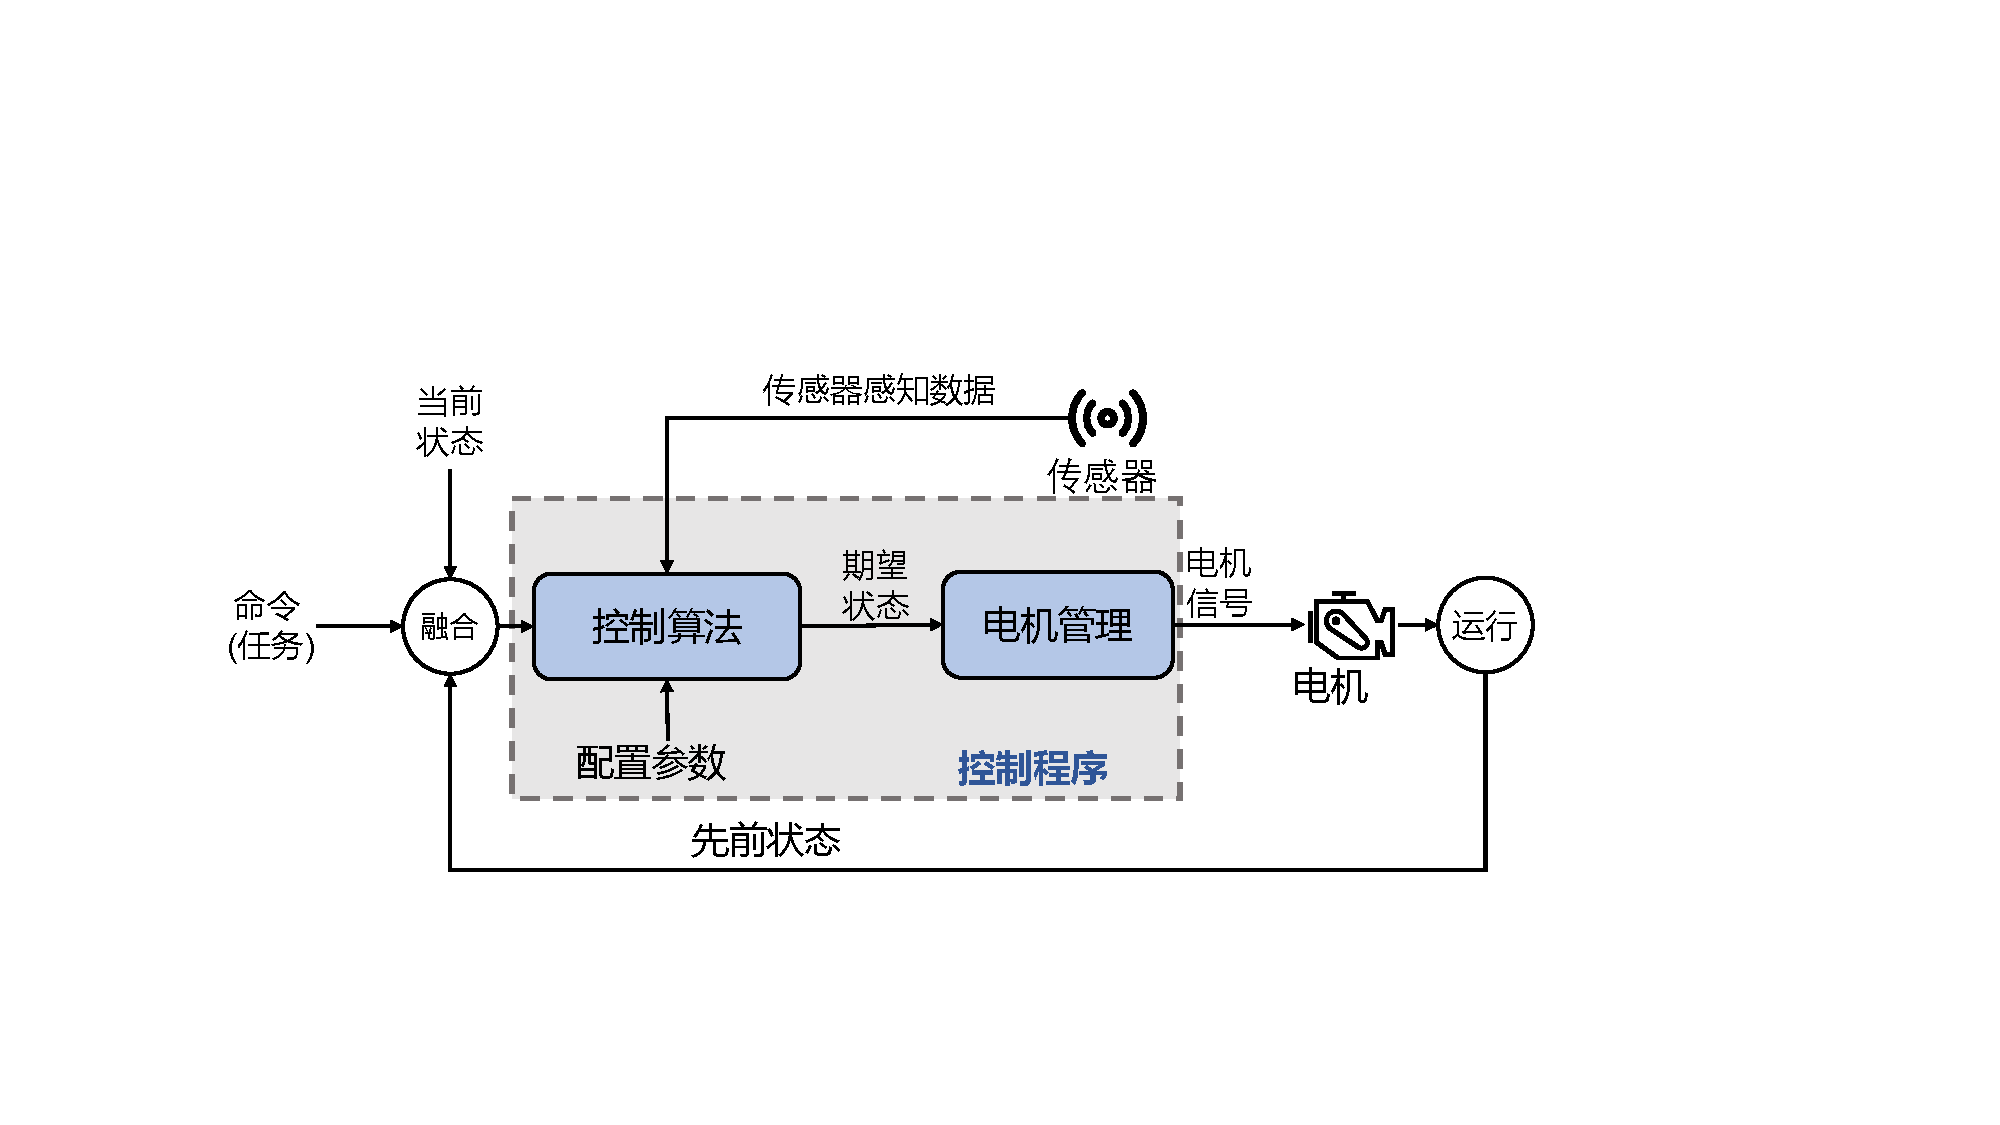
\includegraphics[width=\columnwidth]{fig/background/rawcontrol.pdf}
\caption{无人机飞行控制程序的控制逻辑}
\label{fig:rawcontrol} 
\end{figure}

% 说明存在飞行偏差这一个事实,无人机也是根据这个进行调整的。
然而,真实状态和参考状态并不总是匹配。
如果实际飞行状态和参考状态之间的偏差很小,所以电机可以纠正它,那么飞行状态被认为是稳定的。
否则,飞行状态就被认为是不稳定的。
尽管一些不稳定的状态可以通过发送特定的指令来纠正,但如果偏差累积起来,超过了电机的纠正能力,无人机就会变得不可控。
最终,飞行任务将不得不中断。
图~\ref{fig:des&ach}显示了无人机滚动角度的姿态变化导致了一个不稳定的飞行(红色区域)。
其中实线表示控制器所期望的程度。
虚线表示无人机实际完成的角度,以及底部的直方图(棕色条)表示这两条曲线之间的误差。
从图中可以清楚得观察到,期望的角度和实现的角度在开始时差别不大,但随后增加,导致飞行不稳定。

\begin{figure}[ht]
  \centering
    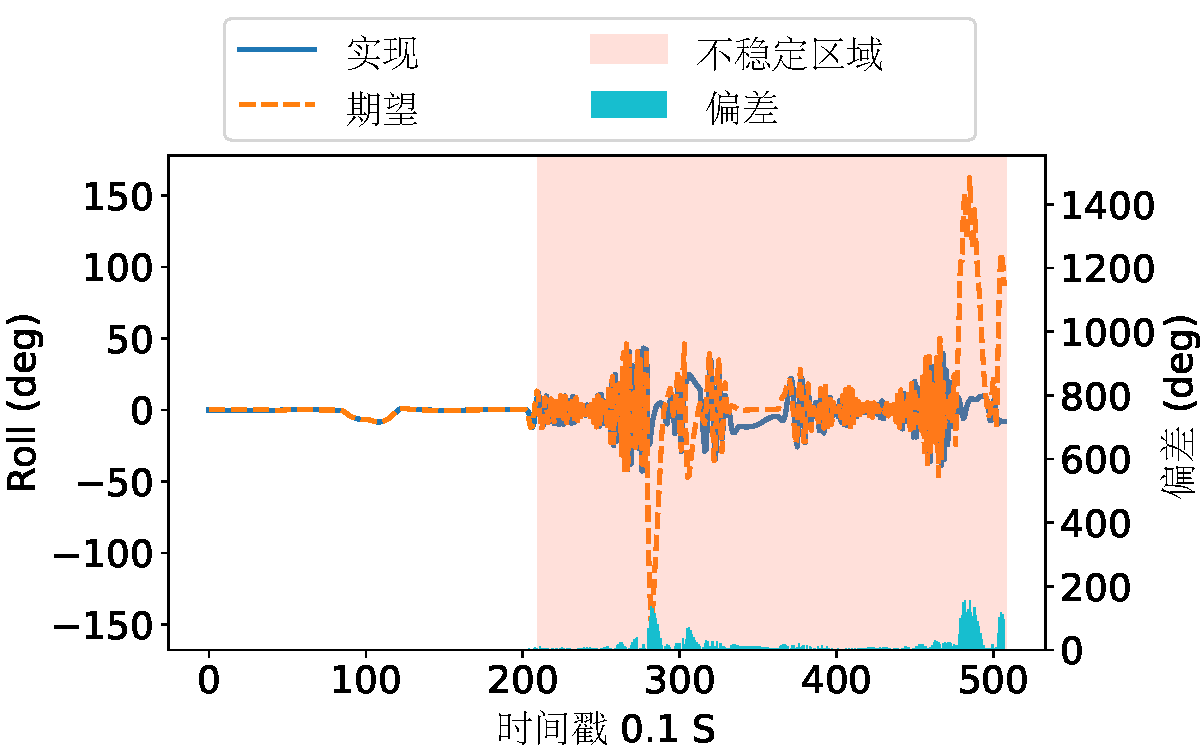
\includegraphics[width=0.9\columnwidth]{fig/background/des&ach.pdf}
\caption{飞行中Roll角的变化.}
\label{fig:des&ach} 
\end{figure}


\subsection{无人机参数控制}\label{subsec:drone_control}
制造商提供由数百个参数组成的可配置控制方案,以支持各种飞行任务。
每个用户/控制台可以通过调整这些参数值来控制无人机,以应对不同的任务场景。
无人机的调试工作很大一部分是对飞行控制参数的调试,广义的飞控参数包含了制导、导航、控制律以及各种控制策略中的可调参数。
一般的飞控都有上百项需要人为调试的参数,有的甚至是几百上千个。而姿态控制作为无人机控制的基础
同时为了保证人员在调试时的安全设定,制造商提供了一种范围控制机制,通过每个参数的预设值范围指导参数选择。

以常用的飞行控制程序\tool{Ardupilot}为例。
代码~\ref{lis:range_bug_code_example} 片断展示了了其飞行控制程序中如何使用参数,\param{PSC\_VELXY\_P},来控制飞行。
在变量声明之后(第6行),\param{PSC\_VELXY\_P}(代码中的\param{k\_param\_pi\_vel\_xy})被分配到一个控制值(第3行)。
飞行控制程序应用这个值来转换角度控制器的增益(第10行至第12行)。
该程序片段同时会校验当前设置的参数值是否会超出了官方预先设定的范围。
通过这种调整机制,无人机的飞行控制程序可以通过更改配置参数从而适应不同的无人机类型,飞行环境和任务需要。
\begin{listing}[ht]
\scriptsize{
\begin{minted}[linenos, firstnumber=8,breaklines,xleftmargin=2em,numbers=left]{c++}
//"PSC_VELXY_P", 0.1, 6;
...
ConversionInfo angle_and_filt_conversion_info[] = {
...
 // PARAMETER_CONVERSION - Added: Jan-2018
{ Parameters::k_param_pi_vel_xy, 0, AP_PARAM_FLOAT, "PSC_VELXY_P" },
}
...
// convert angle controller gain and filter without scaling
for (const auto &info : angle_and_filt_conversion_info) {
    AP_Param::convert_old_parameter(&info, 1.0f);
}
\end{minted}
}
\caption{参数\param{PSC\_VELXY\_P}使用的代码样例}
\label{lis:range_bug_code_example}
\end{listing}


\subsection{无人机安全检查}
% 安全检查
为了减轻潜在的不安全后果,开发者为控制程序设计了各种安全检查机制,以检测异常情况,同时提供反补救措施。
通过应用来自传感器和状态估计的内部无人机信息,这些检查设计了触发条件,以检测特定的突发情况(如崩溃、推力损失)。
当这些条件得到满足时,系统将提出安全警告并启动相应的补救措施。
开发人员通常使用他们的领域知识和经验来构建条件规则。

例如,以 \tool{ArduPilot}为例。
表~\ref{tab:condition}展示了\tool{ArduPilot}工具中的两个安全检查模块及其触发条件。
\emph{崩溃}和\emph{推力损失}。
\emph{碰撞}模块在车辆可能失去控制并撞上物体的情况下解除电机,这可以减少对车辆的损害和对车辆附近的人的伤害。
它在系统中验证四个内部数值,以判断当前飞行不安全:无人机的加速度小于$3m/s$,倾斜角大于$15$度,系统计算的角度误差大于$30$度,无人机速度小于$10m/s$。
\emph{推力损失}模块旨在检测推进系统的硬件故障,即无人机无法再达到要求的姿态和油门输出,因为一个或多个电机在$100\%$的油门下饱和。
如果这种情况持续了很长时间,姿态控制可能无法保持稳定。
该模块验证四个值:控制程序的期望角度大于$15$度,沿$Z$轴的速度为负值,系统计算的角度误差大于$30$度,其油门变得饱和。

\begin{table}[ht]
\caption{Ardupilot官方源代码中的崩溃和推力损失触发条件}
\label{tab:condition}
\centering
\begin{tabular}{c|c|c}
        \toprule[1.5pt]
        \textbf{检查模块} & \multicolumn{2}{c}{\textbf{触发条件}} \\
        \midrule[0.8pt]
        \multirow{2}{*}{崩溃} & 加速度 $ < 3m/s$  &  倾斜角 $ > 15 deg$ \\
        \cmidrule[0.8pt]{2-3}
          & 角度错误 $ > 30 deg$  &  加速度 $ < 10m/s$  \\
        \midrule[0.8pt]
        \multirow{2}{*}{动力损失} & 期望角 $ > 15 deg$  &  Z轴速度为负 \\
        \cmidrule[0.8pt]{2-3}
          & 角度错误 $ > 30 度$  &  油门饱和  \\
        \bottomrule[1.5pt]
\end{tabular}
\end{table}


\section{时间序列预测}
% LSTM和TCN的模型介绍
时间序列预测是一种利用历史和当前数据来预测一段时间内或未来特定时间点的未来值的技术。 
通过分析过去存储的数据,可以做出明智的决策,这些决策可以帮助了解未来趋势。
在机器学习问题中,时间序列的预测被转化为监督学习问题。
算法利用窗口滑动,从时间序列中连续取样,作为生成不同的输入和输出。
下面将介绍两种本文涉及的时间序列预测方法。

\subsection{长短期记忆网络}
长短期记忆网络(Long Short Term Memory,LSTM)~\cite{hochreiter1997long},即长短期记忆网络,一种循环神经网络(Recurrent Neural Network,RNN)~\cite{rnn}的变体。
LSTM专门用于处理有前后关联性的序列数据,具有记忆和长期依赖建模的能力。
LSTM通过添加成为\dquote{门}的结构来控制相关信息的流动,从而解决了传统RNN中存在的梯度消失和梯度爆炸问题,使其能够更好地捕捉长期依赖关系。

LSTM的核心思想是三种不同的\dquote{门}单元,分别为输入门(Input Gate)、遗忘门(Forget Gate)、输出门(Output Gate)。
这些门控单元通过学习的方式来决定是否允许信息通过,从而控制信息在网络中的流动。
其中,输入门决定了当前时刻输入的信息有哪些需要被保留下来,它通过一个激活函数来生成一个0到1之间的值,表示这个信息的权重,也就是信息的重要性。
这个重要性值与输入经过一个tanh激活函数后的值相乘,得到了当前时刻的记忆候选值。
遗忘门决定了前一时刻有哪些信息和记忆要被遗忘。
它使用一个sigmoid激活函数同样生成一个0到1之间的值,表示前一时刻记忆二点重要性。
同样得,这个重要性值与前一时刻的记忆相乘,得到了被保留的记忆。
然后,输出门决定了当前时刻的输出有多少要被传递出去。
它也包含一个sigmoid激活函用于评判输出的重要性,然后与一个tanh激活函数后的值相乘,得到了当前时刻的输出。
最终,LSTM使用当前时刻的输入、前一时刻的记忆和门控单元的输出来更新当前时刻的记忆。
这个更新过程包括遗忘门决定的前一时刻记忆的遗忘部分,输入门决定的当前时刻输入的记忆部分,以及门控单元的输出。
通过这种门控机制,LSTM能够有效地保留和遗忘信息,从而更好地处理长期依赖关系。
它在处理序列变化数据方面比普通的神经网络更好。
诸如高维度、分散性和高噪音等问题。噪声存在的问题,这些问题是传统算法无法处理的问题。

下面将以公式化的方式进行说明。
假设在时间戳$t$,输入为$x_t$,上一时刻的隐藏状态为$h_{t-1}$,上一时刻的细胞状态为$c_{t-1}$,当前时刻的隐藏状态为$h_t$,当前时刻的细胞状态为$c_t$。
LSTM的计算过程可以分为三个门和一个记忆单元,分别为遗忘门、输入门、输出门和细胞状态更新:
\begin{itemize}
    \item \textbf{遗忘门(Forget Gate):}
遗忘门决定哪些信息需要从细胞状态中丢弃。遗忘门的计算公式如下:
\begin{equation}
    f_t = \sigma(W_f \cdot [h_{t-1}, x_t] + b_f)
\end{equation}

\item \textbf{输入门(Input Gate):}
输入门决定哪些新信息需要存储到细胞状态中。输入门的计算公式如下:
\begin{equation}
    i_t = \sigma(W_i \cdot [h_{t-1}, x_t] + b_i)
\end{equation}
\begin{equation}
    \tilde{c}_t = \tanh(W_c \cdot [h{t-1}, x_t] + b_c)
\end{equation}

\item \textbf{更新细胞状态:}
使用遗忘门和输入门的信息来更新细胞状态。更新细胞状态的计算公式如下:
\begin{equation}
    c_t = f_t \odot c_{t-1} + i_t \odot \tilde{c}_t
\end{equation}

\item \textbf{输出门(Output Gate):}
输出门决定当前时刻的隐藏状态$h_t$。输出门的计算公式如下:
\begin{equation}
    o_t = \sigma(W_o \cdot [h_{t-1}, x_t] + b_o)
\end{equation}
\begin{equation}
    h_t = o_t \odot \tanh(c_t)
\end{equation}

\end{itemize}

其中,$(W_f, W_i, W_c, W_o)$ 是权重矩阵,$(b_f, b_i, b_c, b_o)$ 是偏置向量,$([h_{t-1}, x_t])$ 表示将隐藏状态和输入连接起来,$\sigma$ 是sigmoid函数,$\odot$ 表示逐元素相乘操作,$\tanh$ 是双曲正切函数。




\subsection{时间卷积网络}
时间卷积网络(Temporal Convolutional Networks,TCN) ~\cite{bai2018empirical},是一种用于处理序列数据的深度学习模型,他的核心架构是基于卷积神经网络的(Convolutional Neural Network,CNN)~\cite{schmidhuber2015deep}。
TCN能够有效地捕捉序列数据中的长期依赖关系。
与传统的循环神经网络相比,TCN的主要优势在于并行计算的能力和对长期依赖的建模能力。
传统的RNN在处理长序列时容易出现梯度消失或梯度爆炸的问题,而TCN通过使用一维卷积层来捕捉不同时间步之间的依赖关系,避免了这些问题的出现。
此外,TCN还可以并行计算,加速了模型的训练和推断过程。
TCN的核心思想是通过一维卷积层来进行特征提取和建模。
该卷积层可以捕捉局部的时间相关性,并通过多个卷积层堆叠来扩展对于序列中信息的感受视野,从而捕捉更长期的依赖关系。
为了解决卷积层的输出长度问题,TCN引入了残差连接(Residual Connections)~\cite{he2016deep}和空洞卷积(Dilated Convolutions)~\cite{yu2015multi}的技术。
残差连接可以保留原始输入的信息,避免信息的丢失和模型的退化。而空洞卷积则通过增大卷积核的感受野,使得卷积层能够同时捕捉不同时间尺度的依赖关系。
这种方法使CNN非常深,但由于大规模并行处理的优势,它可以被并行处理,无论网络有多深,都可以节省大量的时间。

假设在时间步$t$,输入为$x_t$,TCN的核心是通过卷积操作来捕捉时间序列数据中的长期依赖关系。
TCN的计算过程的公式化描述如下:
\begin{itemize}
    \item \textbf{卷积操作:} TCN使用多层卷积层来提取时间序列数据的特征。
    假设第$l$层卷积层的输入为$z(l-1)$,输出为$z(l)$,卷积核为$w(l)$,偏置为$b(l)$,卷积操作可以表示为:
    \begin{equation}
        z_t(l) = \sigma(w(l) \ast z_{t-k}(l-1) + b(l))
    \end{equation}
    其中$\ast$表示卷积操作,$\sigma$是激活函数,$k$是卷积核的大小。

    \item \textbf{残差连接:}为了加快训练速度和提高模型性能,TCN通常采用残差连接。
    \begin{equation}
        z_t(l) = z_t(l-1) + z_t(l)
    \end{equation}

    \item  \textbf{池化操作:} 池化操作有助于减少特征的维度,提取最重要的特征。常用的池化操作包括最大池化和平均池化。
    最大池化的计算公式如下:
    \begin{equation}
        z_t(l) = \max(z_{t-j}(l))
    \end{equation}
    其中$j$是池化窗口的大小。

    \item \textbf{输出层:} 最后一层卷积层的输出可以通过全连接层或者其他适当的操作来得到最终的输出。假设最后一层卷积层的输出为$z(l)$,输出层的计算可以表示为:
    \begin{equation}
        y_t = \text{softmax}(W_{\text{out}} \cdot z_t(l) + b_{\text{out}})
    \end{equation}
    其中$W_{\text{out}}$是输出层的权重矩阵,$b_{\text{out}}$是输出层的偏置向量 。
\end{itemize}


\section{不变量验证}
不变量的字面是表达\dquote{不会改变的量}。
它是一种重要的数学和物理方法,用于检验系统在不同条件下是否遵守某些基本规律或性质。
在数学和物理学中,不变量是指在系统变化过程中保持不变的物理量或性质。
在工程学中,不变量验证通常用于检验工程模型的稳定性和准确性。
在现实世界的应用中,这种不变量是由开发者手动分配的,或者由程序分析自动生成。
例如,在有限元分析中,工程师可以利用不变量验证来确保模型在不同网格密度下的数值解是否收敛到正确的结果。
通过验证一些数学量(如误差估计、残差等)的不变性,工程师可以评估模型的准确性和可靠性。
除非发生模式偏差或外部影响,否则对象的变量应始终遵循不变性约束。

同时也是不变量的这一特性,如果对象约束出现明显偏离于不变量约束的模式,则会被认为是出现了异常。
例如,DAIKON~\cite{ernst2001dynamically}提取一个明确的程序不变式,在修改代码时可以保留程序属性,并利用它来检测运行时异常。
运行时验证~\cite{rocsu2009runtime}利用flow invariant,通过检查控制流来验证合法的程序状态转换。
S3FD~\cite{zhang2017s3fd}提出了一个基于尺度的不变性,以实现实时人脸检测,而不考虑相机距离。
Choi~\cite{choi2018detecting}设计了一个机器人车辆的控制不变性,以监测异常控制数据来提出攻击警告。
这些研究表明,不变性检查可以描述广泛的面向软件(即网络)的异常情况。


\section{遗传算法模糊测试}
遗传模糊测试(Genetic Fuzzing)是一种结合遗传算法(Genetic Algorithm,GA)和模糊测试(Fuzzing)的测试技术,用于发现软件系统中的漏洞和错误。
它通过自动化地生成、变异和评估输入数据,以探索软件中存在的异常行为,且可以是动态的或者静态的。
遗传算法是一种启发式优化算法,模拟了生物进化的过程。
自然界生物在周而复始的繁衍中,基因的重组、变异等,使其不断具有新的性状,以适应复杂多变的环境,从而实现进化。
遗传算法精简了这种复杂的过程而抽象出一套数学模型,用较为简单的编码方式来表现复杂的现象,并通过简化的遗传过程来实现对复杂搜索空间的启发式搜。
它通过使用基因表示解空间中的候选解,并利用选择、交叉和变异等操作来搜索最优解。
在遗传模糊测试中,遗传算法被用于生成和演化输入数据,以尽可能地覆盖软件系统的不同执行路径。
而将遗传算法与模糊测试相结合,可以对模糊测试的目标进行全局寻优,提高模糊测试的覆盖准确度,降低无效测试的概率。
遗传模糊测试的流程通常包括以下几个步骤:

\begin{itemize}
  \item \textbf{初始化种群:} 初始时,随机生成一组输入数据,称为种群。每个输入数据都被视为一个个体,具有一定的基因表达。
  \item \textbf{评估适应度:} 将种群中的每个个体输入到待测试的系统中,并评估其执行结果。适应度函数用于评价个体在测试中的表现,通常是基于代码覆盖率、错误率或其他测试目标。
  \item \textbf{选择操作:} 根据个体的适应度,在种群中选择一部分个体作为父代,用于下一代的繁殖过程。通常采用轮盘赌选择或排名选择等策略。
  \item \textbf{交叉操作:} 从选定的父代中,随机选择两个个体,并通过交叉操作生成新的个体。交叉操作模拟了生物遗传中的基因交换过程,以产生更多的遗传变异。
  \item \textbf{变异操作:} 对新生成的个体进行变异操作,以引入更多的随机性和多样性。变异操作模拟了生物遗传中的基因突。
  \item \textbf{更新种群:} 将生成的新个体加入到种群中,并删除一部分适应度较低的个体,以保持种群的规模稳定。
  \item \textbf{迭代终止:} 根据预设的终止条件(例如达到最大迭代次数或满足特定的测试目标),决定是否终止遗传模糊测试的过程。
\end{itemize}

\section{深度确定性策略梯度DDPG}
强化学习(Reinforcement Learning,RL)是一种机器学习方法,旨在通过智能体(Agent)与环境的交互学习如何做出最优决策。
在强化学习中,智能体通过观察环境的状态,采取动作,并获得奖励分数来学习如何在不同状态下做出最优的决策策略。
强化学习的目标是通过与环境的交互,使智能体学会最大化累积奖励的策略。

深度强化学习策略(Deep Deterministic Policy Gradient,DDPG)~\cite{lillicrap2015continuous}是一种基于深度学习的强化学习算法,专门用于解决连续动作空间的问题。
DDPG算法的核心思想是使用深度神经网络来近似值函数和策略函数。它包含两个主要的网络:一个是Actor网络,用于学习策略函数,根据当前状态输出一个动作;
另一个是Critic网络,用于学习值函数,根据当前状态和动作输出一个值函数估计。
DDPG算法通过不断地在经验回放缓冲区中采样并更新这两个网络,来优化策略和值函数的参数。

DDPG算法的步骤如下:
\begin{itemize}
  \item \textbf{初始化:} 初始化Actor网络和Critic网络的参数。
  \item \textbf{环境交互:} 根据当前状态使用Actor网络选择一个动作。
  执行选择的动作并观察环境反馈的下一个状态和奖励。
  将状态、动作、奖励和下一个状态存储到经验回放缓冲区中。
  从经验回放缓冲区中随机采样一批数据。
  \item \textbf{更新Critic网络的参数:} 根据下一个状态和Actor网络的目标动作,使用Critic网络计算目标Q值。
  使用Critic网络计算当前状态和动作的Q值。
  使用目标Q值和当前Q值之间的均方差作为损失函数。
  通过梯度下降法最小化损失函数来更新Critic网络的参数。
  \item \textbf{更新Actor网络的参数:} 根据Critic网络的输出和Actor网络的动作,计算Actor网络的策略梯度。
  通过梯度上升法最大化策略梯度来更新Actor网络的参数。
  \item \textbf{条件停止:} 重复上述步骤,直到达到预设的停止条件
\end{itemize}

DDPG算法通过不断地在经验回放缓冲区中采样和更新网络参数,逐渐优化策略和值函数,从而学习到在连续动作空间中最优的策略。


\chapter{不变量验证的可靠安全检查方案}
\section{引言}
无人机已经成为商业、工业、娱乐和执法的重要支援设备~\cite{chabot2018trends,banos2020assessment,patino2009adaptive,shukla2016application,huang2021multi,li2018uav}。
随着无人机越来越多地被用于关键任务,客户对无人机飞行的可靠性和稳定性有很高要求。
因此,无人机的软件开发者建立了一种安全检查系统来检测和缓解此类飞行过程中的安全问题。
这样的系统通常有不同的模块来处理不同的安全问题,如无人机坠毁、电机推力损失、角位置不平衡等。
模块通过应用它们的条件规则来检验特定的内部监测值(如特定角度)来判断相应的安全问题是否发生。
当检测到问题时,系统提供补救措施,例如,在检测到推力损失时启动动力助推来帮助恢复正常飞行,在检测到碰撞时切换到降落模式确保无人机能够安全着陆。
对于目前的实际应用,安全检查系统的规则通常是由较为简单的布尔语义(Boolean)并结合阈值判断的方法来进行构建。
而设计的相应的断条件一般由开发者根据自己的开发经验来指定,这种由人工确定的规则会带来一些问题。


受限于简单的布尔语义这种线性表达方式对于数据的描述,以及开发者不可靠的专业经验,当前的安全检查方式对特定的安全问题的检测和处理仍存在较大的疏漏。
特别是在处理一些复杂的事件时,当前的安全模块容易导致漏报或误报。
由这种漏报或误报引起的人身伤害、财产损失和其他损害的实际事故在不断增加。
研究~\cite{choi2020cyber}通过实验表明了一个现实的疏漏场景。
它通过实验构造了一种特殊的碰撞场景,侧面撞墙,这种碰撞由于碰撞角度不满足系统设定的检测阈值,从而使得碰撞安全检查无法检测到危险情况。
这种导致漏报的事件称为\emph{不足事件},这类事件不会触发安全系统的任何补救对策,从而导致无人机撞到地面或人。
此外,现实中还存在一种情况,以航空灾难~\cite{boe18,boe19}为例,气流变化错误地触发了Boeing-737-Max的机动特性增强(姿态检查模块),导致错误报警。
这种误报触发了安全系统的补救行为,但是由于误报,这种补救行为反而与驾驶员的飞行行为相冲突,最终导致了飞机坠毁。
本章节研究将这些类型的事件称为\emph{过度事件}。
上述证据表明,初级的基于条件的安全检查不足以满足安全要求,因为其线性条件不能准确地描述这类复杂的不安全事件。

这些不安全的事件不仅需要被识别,而且需要给予正确的安全处理,即补充漏报和减轻误报带来的问题。
先前针对无人机的检测研究~\cite{choi2018detecting, fei2018cross, piper, choi2020software, ahn2019learning}主要是检测飞行过程中的异常情况。
虽然他们可以提高检测被忽视的异常情况的能力,但他们不能正确处理误报,这仍然会造成严重的后果。
因此,对安全检查模块的迫切要求是检测这些不安全事件,同时准确提供适当的补救措施。

本章节通过提出一种不变量可靠安全检查方案,并实实现了原始的辅助系统\deccheck 来应对这些挑战。
\deccheck 为不安全事件创建了特征描述,并且进一步利用一个检测器来识别它们,同时提供适当的应对措施。
受不变量(一种描述数据中异常模式的方法)的启发,\deccheck 建立了一种状态不变量,用于生成不安全事件状态模式的特征描述。
状态不变量是由飞行状态(如角位置和角速率)、传感器数据(如GPS和陀螺仪)和无人机的控制逻辑共同提取的。
它可以根据当前的状态和传感器读数来估计下一个时间的状态,而实现的状态偏离估计值,实际数据与估计数据产生偏差则被认为是异常的。
利用状态不变量,系统提取不安全事件的分段特征,然后训练卷积神经网络(CNN)~\cite{cnn}检测器来准确识别它们。
最后,状态变量和检测器被整合到一个控制程序中,以协助安全检查,该系统持续捕捉实时数据以检测不安全事件。
当检测到\emph{不足事件}时,\deccheck 补充警告,当检测到\emph{过度事件}时,中断错误的警告。

\section{安全检查存在的问题}\label{sec:check_problem}
安全检查模块的设计本意是对无人机进行一定程度的保护和安全补救。
然而,由各种条件组合而成的检查模块并不能可靠地描述一些不安全事件,进而无法可靠地识别这些不安全事件。
这些不安全事件被归为两类,\emph{不足事件}和\emph{过度事件}。
\emph{不足事件}是轻微的或特殊的事件,它是一个检查模块的目标检测事件但实际上没有触发或只部分触发检查条件。
这种事件使得检查模块不发出任何警告,造成漏报,从而进一步造成硬件或个人的损害。
相反, \emph{过度事件}是事件的飞行数据状态满足检查条件的一些瞬时事件或噪音,但是由于其持续时间较短的属性,事件本身并不会造成后续影响。
然而,如果一个检查模块有补救措施,这种事件仍会触发补救措施,这些补救反而会影响无人机的飞行控制。
这种\emph{过度事件}将引发不适当的补救措施,造成失控。

本节使用一个预先实验来说明 \tool{Ardupilot}~\cite{ardupilot}中安全检查存在的问题,并引出为什么要使用更高Precision的识别和更准确的应对措施。
具体来说,\emph{轻微碰撞}(在碰撞检查的事件下),如侧面碰撞或反弹的正面碰撞,可能不满足部分规则(如倾斜角度)。
但是,它还是会影响到无人机的完整性或进一步造成影响(例如,轨迹偏差和硬件损坏)。
短暂的\emph{阵风晃动}(超过推力损失检查的事件)可能会触发所有的推力损失规则来激活电机助推。
但是短暂的阵风会立即消失从而使助推成为一个不恰当的操作,导致飞行器向一个意外的方向移动或其他故障状态。
为了直观地说明安全检查对这些事件的反应,此处分别进行了$100$次的\emph{轻微碰撞}和$100$次的\emph{阵风晃动}飞行(实验细节将在后续实验章节中补充)。
表~\ref{tab:check_crash_err}记录了所有的飞行记录和它们的错误信息。
在表中,\emph{安全检查错误}表示一个事件触发了检查规则和补救措施,控制程序认为无人机处于紧急情况(致命)。
\emph{其他系统错误}表示其他系统模块(如控制模块和任务执行模块)报告的额外异常,控制程序认为无人机不稳定但不致命。

\begin{table}[ht]
\caption{不安全事件影响下无人机出现的错误信息}
\label{tab:check_crash_err}
\centering
\begin{threeparttable}
\begin{tabular}{c|c|c|c|c|c}
        \toprule[1.5pt]
        \multirow{2}{*}{不安全事件} & \multirow{2}{*}{安全检查错误} & \multicolumn{4}{c}{其他系统错误}\\
        \cline{3-6}
          &  & GPS故障 & 潜在不良姿态 & 潜在失控安全 & 过度震动补偿  \\
        \midrule[0.8pt]
         100~轻微碰撞 & 2 坠毁 & 88 & 89 & 89 & 12  \\
         
         100~阵风晃动 & 44 动力损失 & 1 & 1 & 1 & \diagbox{}{}  \\
        \bottomrule[1.5pt]
\end{tabular}
% \begin{tablenotes}
% \footnotesize
% \item[*] \textbf{G}: GPS故障; \textbf{B}: 不良差异(姿态估计不良); \textbf{F}: 触发失控安全;  \textbf{E}: 激活了过度振动补偿
% \end{tablenotes}
\end{threeparttable}
\end{table}


实验结果中可以观察到,碰撞检查模块只检测到$2$个碰撞。
它漏掉了$98$个\emph{轻微碰撞},同时可以看到这些事件还造成了许多其他系统错误信息(包含$88$个\emph{GPS故障},$89$个\emph{潜在不良姿态},$89$个\emph{潜在失控安全},以及$12$个\emph{过度振动补偿})表明这些轻微的碰撞导致了极其不稳定的状态。
如果无人机迎面撞上一个物体,可能会直接导致无人机静止或下降。
如果无人机以一定的角度撞到一个轻的物体,或者冲击力小于正面碰撞,这样的碰撞会导致航向改变,并进一步导致随机方向的弹开。
这两种情况都会对飞行器的安全(如部件损坏)和周围环境(如人员受伤)产生关键影响。
从上述实验结果观察,\emph{轻微碰撞}受到的关注要少得多。
至于\emph{阵风晃动},它引发了$44$个的推力损失信息,但导致的其他系统错误较少(几乎没有引起不稳定)。
然而,过于敏感的安全检查模块启动了电机助推,导致$18$次飞行的轨迹出现偏离,每次的偏差均大于$1$米。
这样的电机助推将大大影响无人机的飞行控制,应该更加谨慎地启动。
上述两个例子表明,在处理\emph{轻微碰撞}和阵风等不安全事件时,初级安全检查系统不能满足可靠性和稳定性要求。

\section{挑战与解决思路}

\subsection{问题难点及挑战}
在处理\emph{不足事件}和\emph{过度事件}所带来的安全事件问题需要面临以下挑战。

\begin{itemize}
    \item \textbf{挑战 1: 如何对事件生成准确的特征描述?} 
    上述说明案例说明和以往研究工作已经表明了使用线性阈值的方法无法有效描述一个安全事件,从而导致无法提供正确的应对措施。
    同一种类型的不安全事件本身就具有多样性,相互之间因所处环境或者飞行状态的不同导致数据模式难以统一。
    但是某些特定情况下不同安全事件之间也可能存在一定的相似性。
    因此,不安全事件需要匹配适当的特征描述,以消除同类型事件中的数据模式差异,同时加强不同事件之间的区分度。
    
    \item \textbf{挑战 2: 如何准确地识别事件?}
    由于生成的特征描述是非线性的数据,原始采用阈值的方法则不能用来进行判断,因此需要一个高效准确的检测器来准确识别他们。

    \item \textbf{挑战 3: 如何正确地处理事件?}
    不安全事件造成的严重后果处理漏报带来的危险外,还有误报所造成的不合理的补救措施。
    在识别了不安全事件的情况下,软件仍然需要提供正确的补救措施,以防止错误的警报和被忽视的异常情况。
    
\end{itemize}


\subsection{解决思路}

正如之前所展示的内容,控制程序中的安全检查在面对不安全事件时可能会受到影响(即,\emph{不足事件}和\emph{过度事件})。
为了解决这样的潜在安全问题,本章节设计了一个辅助系统,\deccheck ,来正确处理不安全事件。
\deccheck 的核心思想是用一个事件检测器来补充安全检查模块,识别不安全事件并提供相应的辅助操作。
考虑到无人机的飞行场景,同一类型的不安全事件可能有不同的飞行状态模式(同样导致坠毁但角度各不相同)。
因此,为了统一同类型事件的数据模式,方案提出了一种基于不变量的特征,利用估计的偏差而不是原始数据,从飞行数据中提取特征描述(解决挑战 1)。
通过这样的特征,系统进一步实现了机器学习检测器检测器来识别这些事件(解决挑战 2),并提供辅助操作:对于\emph{不足事件},系统为检查模块补充警告;对于\emph{过度事件},本章节提前分析哪些模块会受到影响,如果检查被触发,系统会验证是否由\emph{过度事件}引起,以确定消除补救措施(解决挑战 3)。

\section{方案}
该节将展示解决方案,并介绍了 \deccheck 的概况,这是一个用于安全检查模块的辅助系统,促进无人机在面对不安全事件时的处理准确率。

\subsection{概览}
辅助系统(如图~\ref{fig:check_overview}所示)包括一个\emph{离线分析}阶段和一个\emph{机载辅助}阶段。
在\emph{离线分析}阶段(黄色标签),系统利用模糊测试软件来寻找不安全事件(\circled{1})。
人为手动分析哪些检查模块会受到影响,并根据其类别创建一个解决方案,即 \emph{不足事件}或 \emph{过度事件}(\circled{2}到 \circled{5})。
然后,对于此类事件,\deccheck 建立了一个数据收集平台。
它进行飞行实验,收集常规飞行(没有任何不稳定的飞行)日志和不安全事件日志(\circled{6})。
利用常规飞行数据,\deccheck 提取了能够准确预测状态变化的状态状态不变量(\circled{7})。
随后,\deccheck 为数据生成分段不变的不同特征,并创建一个检测器来识别它们的类别(\circled{8} to \circled{10})。

在机载辅助阶段(蓝色标签),对于未知的飞行日志,系统创建相应的特征,并通过检测器识别其类别(\circled{1}到\circled{3})。
根据类别和生成的方案, \deccheck 提供适当的补救措施。

\begin{figure}[ht]
   \centering
    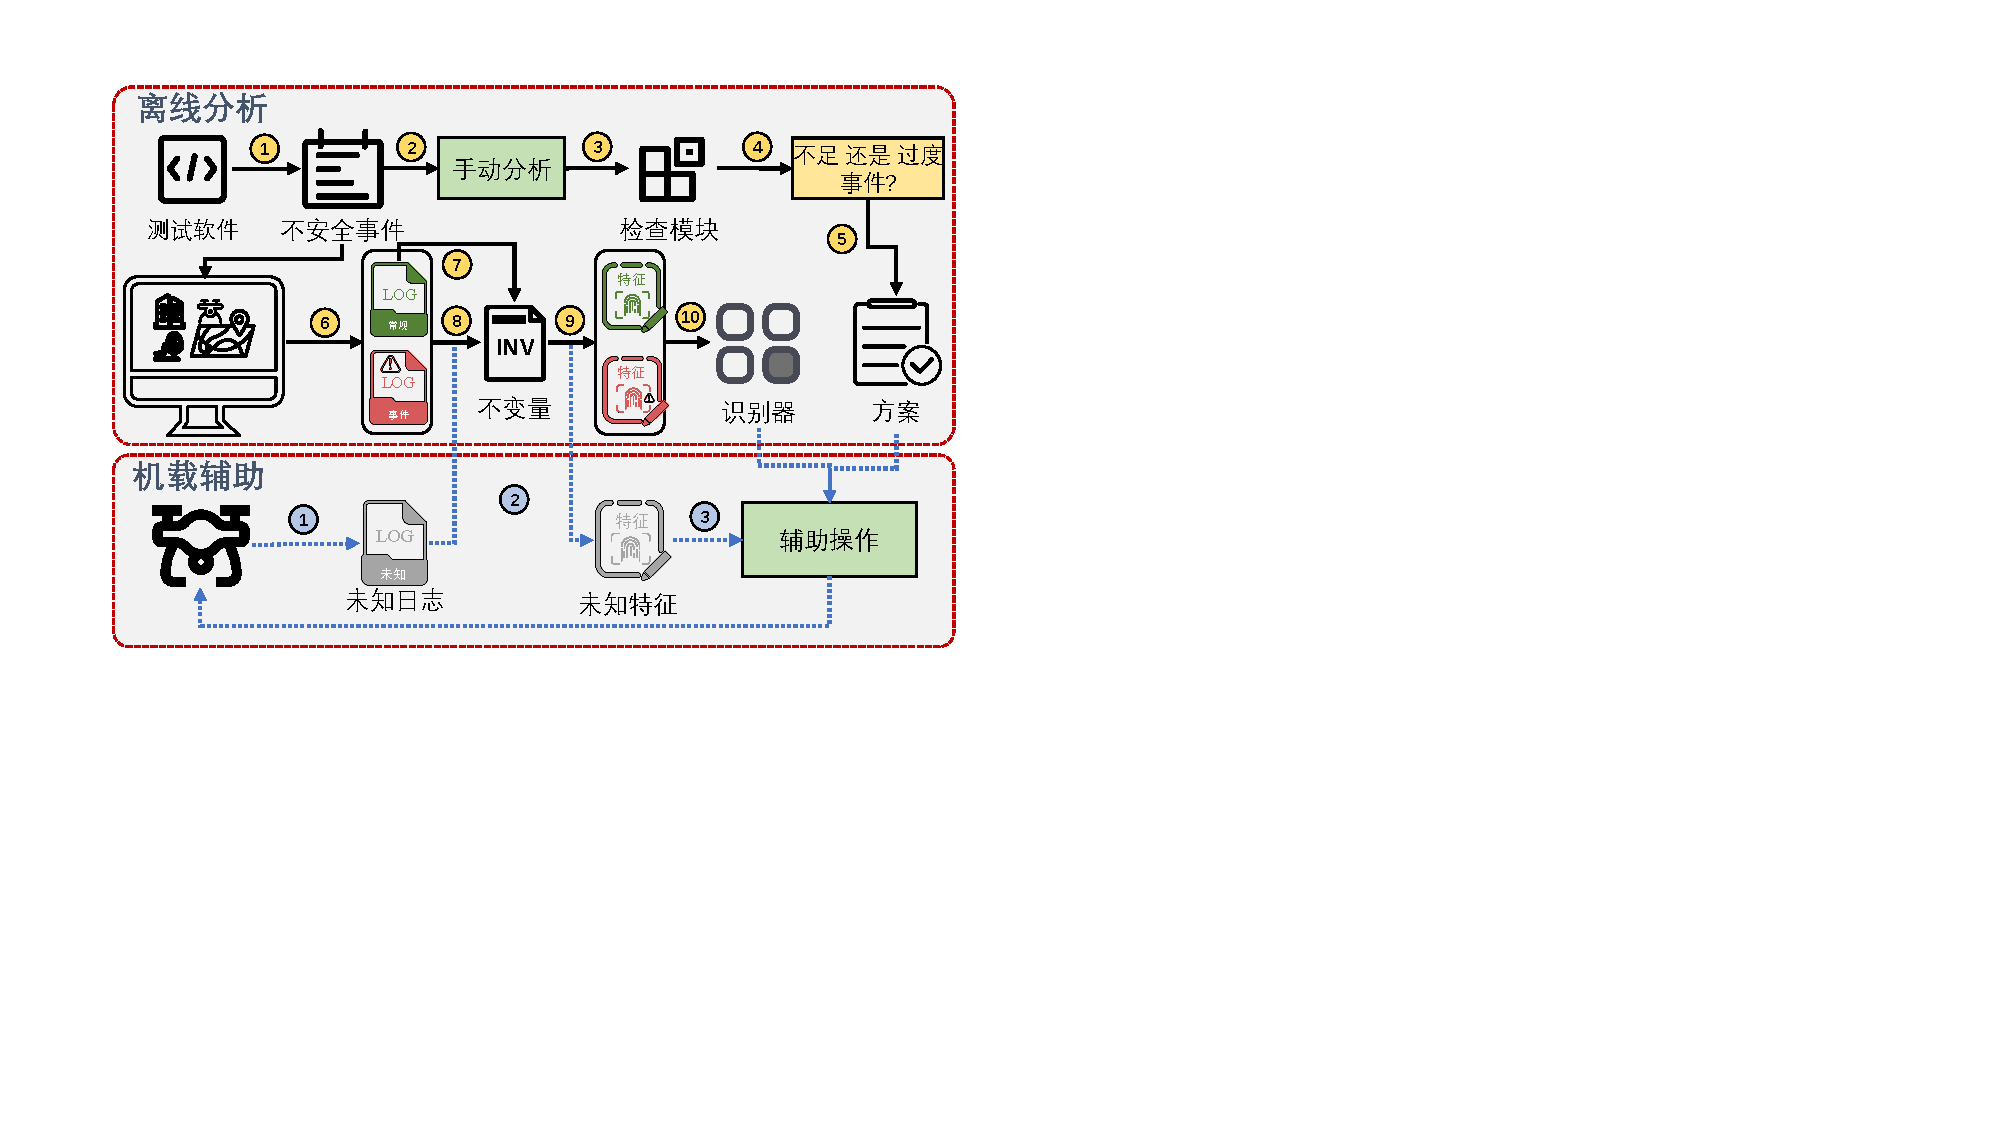
\includegraphics[width=\linewidth]{fig/check/overview_check.pdf}
\caption{\deccheck 流程和子模块}
\label{fig:check_overview} 
\end{figure}


\subsection{事件发现和分析}
\deccheck 首先应用模糊测试方法~\cite{choi2020cyber}来发现不安全事件。
对于不同类型的安全检查模块,\deccheck 使用不同的策略。
参考模块的官方文档或源代码,如果模块补救描述中包含控制操作或电力系统变化,则策略设置为搜索那些触发条件但不引起不稳定的事件(\emph{过度事件});如果模块补救只提出警告或简单的飞行模式切换,则策略设置为搜索那些引起不稳定但不触发条件的事件(\emph{不足事件})。
而根据它们的类别,\deccheck 采用不同的反应方案:(1)对于\emph{不足事件},\deccheck 为控制程序会发布一个新的警告,(2)对于\emph{过度事件},\deccheck 则中断它们的补救工作。


\subsection{数据收集}
由于不变量和检测器的生成需要数据训练,而无人机没有标准的数据集,所以实验手动发起数据采集,建立数据集。
而考虑到在不同的环境中很难提供真实的飞行,而且造成硬件损坏的概率很高,所以系统应用\tool{Airsim}模拟器~\cite{airsim2017fsr}来进行虚拟飞行实验。
\tool{Airsim}是一个真实的无人机飞行器模拟器,开发者可以获得内部飞行信息,包括飞行器的姿态、环境风速、碰撞信息和飞行日志。

\deccheck 进行两种实验来收集相应的数据--常规飞行和不安全事件。
常规飞行实验记录了没有任何物理事件影响的常规飞行状态数据。
不安全事件实验是针对不同场景下的每种不安全事件进行的。
每个飞行日志包含多个条目,由状态信息(如角度位置、加速度和油门速度)、传感器数据(如GPS、陀螺仪和加速度计)以及时间戳索引组成。
特别是,不安全事件日志只记录从事件开始到结束的时间戳。


\subsection{飞行状态不变量}
正如先前章节~\ref{moti:pre_study}中所介绍的有关无人机的飞行控制逻辑。
除非有干扰事件发生,控制算法的生成期望结果与实际的实现结果通常保持一个较小的偏差(甚至没有偏差)。
利用这一特性,\deccheck 建立一个状态不变量来模仿无人机状态估计逻辑。
在理想情况下(无干扰的常规飞行),实际状态将更接近于不变量预测的参考状态。
相反,如果实际的飞行状态与状态不变量给出的状态存在较大偏差,则认为当前状态偏离了不变量规定的飞行状态模式。
偏差值可以用来衡量当前状态的偏离程度。
以下通过\emph{飞行数据预处理}和\emph{状态不变量提取}两个小章节介绍如何处理数据以及生成不变量。

\subsubsection{飞行数据预处理}
所收集的飞行日志为一个列表,每个日志内都包含了飞行信息,如常规位置、陀螺仪传感器数据和时间戳。
但其中并不是所有的数据都对不安全事件的影响敏感。
考虑到不安全事件主要影响飞行姿态,系统采用了与姿态相关的状态和传感器数据:
(1)状态数据中的角位置和角速率,每一个都包含三个欧拉角,即Roll、Pitch和Yaw;
(2)从陀螺仪和加速度计获得的数据,每一个都包含沿X、Y和Z轴的三个数值。
同时,由于状态和传感器数据具有不同的更新频率,系统对具有高更新频率的数据进行采样,并使用时间戳作为索引,使其与具有较低更新频率的数据保持一致。
最终,时间戳$t$的数据向量形式为$v_t=\{a_t, e_t\}$,其中$a_i$和$e_i$是状态和传感器数据。
为了消除数据分布造成的不良影响,系统通过\tool{最小-最大尺度缩放}将特征值归一到$[0, 1]$之间。


\subsubsection{状态不变量提取}
由于物理世界中的不安全事件的飞行状态是复杂的、非线性的,在拟合模型中传统的线性拟合方法效果较差。
\deccheck 利用\tool{长短期记忆网络(Long Short Term Memory Networks,LSTM)}~\cite{hochreiter1997long}这种非线性学习模型方法来生成状态状态不变量,图~\ref{fig:check_invariant}总结了其原理和功能。
从功能上讲,状态不变量以$h$的连续向量$\{v_{t-h-1},...,v_{t-1},v_t\}$作为输入,并返回下一个时刻数据$v_{t+1}'$中的参考状态$a_{t+1}'$的最大条件概率预测值。

在训练阶段,模型通过最小化\tool{Mean Squared Error (MSE)}~\cite{4775883}来迭代更新其权重,从而减少预测的参考状态$a_{t+1}'$与地面真实状态$a_{t+1}$之间的偏差。
例如,假设一个样本数据是$\{v_1,v_2,v_3,v_4,v_5\}$。
如果设置窗口大小$h$=3,则该样本数据可以划分为输入和输出对$\{v_1,v_2,v_3; a_4\}$和$\{v_2,v_3,v_4; a_5\}$。
该模型通过学习$\{v_1,v_2,v_3\rightarrow a_4\}$的这种输入输出关系来更新其内部的网络模型权重,从而达到在输入为$\{v_2,v_3,v_4\}$时有最高的概率输出$a_5$。

\begin{figure}[ht]
  \centering
    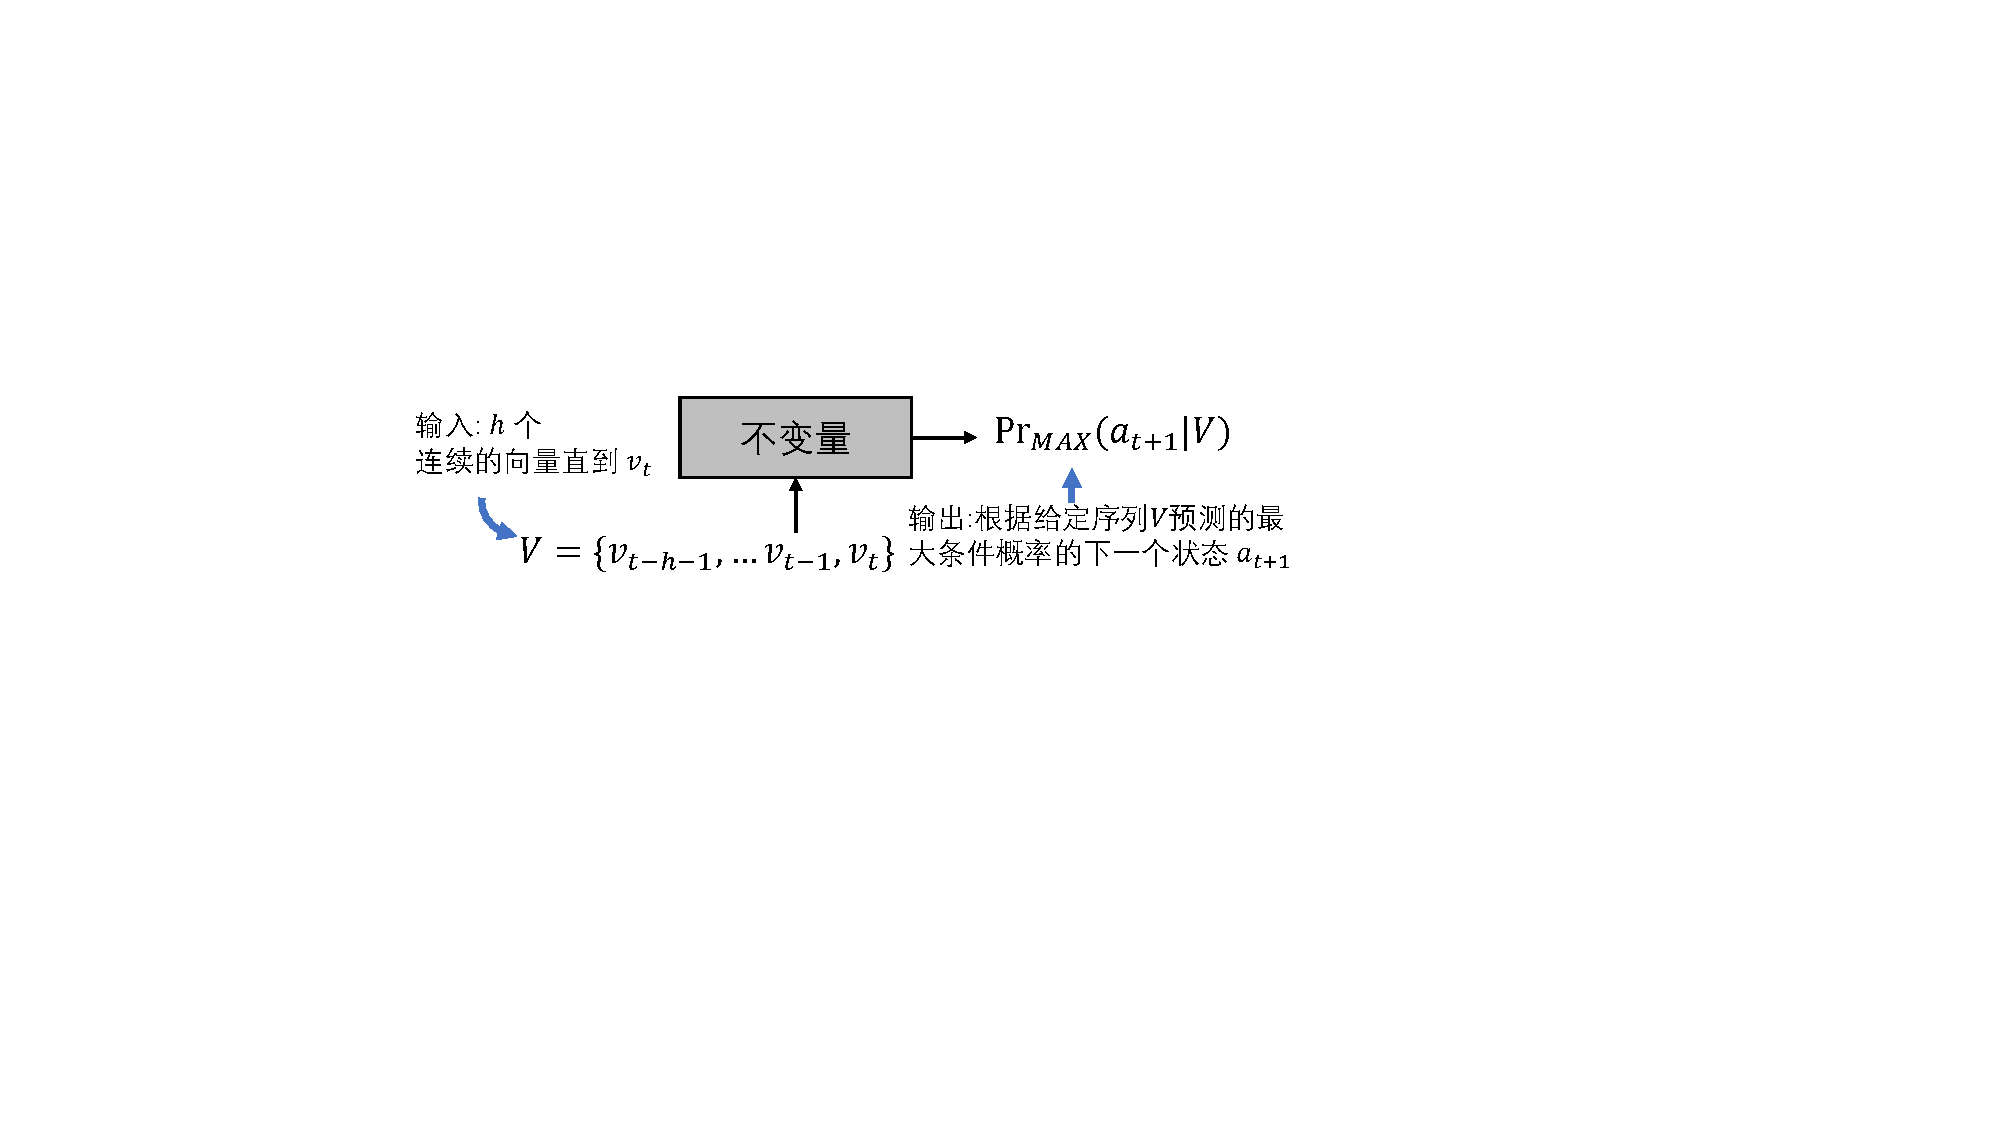
\includegraphics[width=\columnwidth]{fig/check/invairant.pdf}
\caption{飞行状态不变量的功能说明}
\label{fig:check_invariant} 
\end{figure}  

\subsection{不安全事件识别}
为了创建一个检测器来识别不安全事件,\deccheck 首先为每个不安全事件数据提取特征描述。
而为了确保同一类型的事件具有相同的特征模式,系统使用状态不变量来提取特征描述(称之为 \emph{段不变量偏差})。
该特征可以描述段中的异常数据,并保留系列值之间的关联性。
这种带有上下文相关属性的段特征可以减少单一异常数据的影响。
系统应用这些特征训练一个检测器来准确检测飞行中的这些不安全事件。
下文将详细描述从事件数据中提取特征、检测器训练和潜在不安全事件检测三个方面详解系统本身。

\subsubsection{特征描述提取}
给定一个事件数据,\deccheck 首先将其预处理为连续向量$V\{v_1,v_2,...,v_{n1}\}$,其中长度$n1$是事件的持续的时间戳长度。
由于事件有不同的持续时间(即长度$n1$),\deccheck 利用向量的滑动采样方法来生成具有相同形式的多个片段,其中长度与飞行状态包含元素个数的数量相同(在实现中长度为$6$)。
因此,一个事件数据可以产生多个片段$S_i$,规则如下。
\begin{equation}
S_i = \{v_i,v_{i+1},...,v_{i+5}\}, i\in[1,2,..., n-5]
\end{equation}
对于片段$S_i$,系统应用状态不变量来创建段预测$A'_i$,并计算它们之间的偏差称之为\emph{段不变量偏差}特征$SID$。

假设一个段为$S\{v_{1},v_{2},...,v_{6}\}$,下面将解释状态不变如何生成相应的预测段$A'$。
为了确保$S$能够生成相同大小的预测段$A'$,系统首先向$S$插入$h-1$行(与第一行的值相同),以获得填充段$S_{fill}$。
状态不变量使用这个填充段$S_{fill}$作为输入来生成预测状态段$A'\{a_1',a_2',...,a_6'\}$,规则如下。
\begin{equation}
a_j' = SI({v_j,v_{j+1},...,v_{j+h-1}}), j\in[1,2,...,6]
\end{equation}
其中$SI$是状态不变量,$v_j$是$S_{fill}$中索引为$j$的特征向量。
随后,系统选择$S$中的状态数据$A\{a_1,a_2,...,a_6\}$,计算与预测段$A'$的偏差,生成段不变差特征$SID = \Vert A - A' \Vert$。

\subsubsection{识别器训练}
训练之前首先要为事件提取的特征手动标记地标记标签。
考虑到$SID$是一个矩阵,先前的研究~\cite{girshick2015fast,shin2016deep}表明CNN~\cite{cnn}对矩阵形式的特征有更高的分类效率,因此\deccheck 利用CNN来创建检测器。
虽然CNN可以从原始数据中自动提取特征,但段不变差提取了更高层次的特征,考虑了状态变化的背景。
与\emph{段不变差}特征相结合,CNN有效地利用了矩阵值的位置关系,增强了检测器的有效性,消除了异常值分布的影响。

\subsection{潜在不安全事件识别}
当获得飞行状态不变量和检测器后,\deccheck 将被部署于无人机中用来监测飞行状态。
由于无人机硬件(如\tool{Pixhawk}~\cite{meier2011pixhawk}和\tool{TauLabs}~\cite{ebeid2018survey})通常使用STM32等性能较弱的芯片,\deccheck 采取异步检测,避免影响控制程序的运行。
它不断捕捉飞行状态和传感器数据的机载计算机来检测不安全事件。
每当它捕捉到六个信息条目时,它就会生成分段不变差特征,并应用检测器来识别当前的飞行状态。
根据检测到的类别,\deccheck 为控制程序提供补充建议。
(1)如果该类别属于\emph{不足事件},系统会发出警告并提供中断飞行的建议。
(2)如果该类别属于\emph{过度事件},并且安全检查触发了特定的检查模块,系统将清除警告并提供继续飞行的建议。

\section{实验结果及分析}
本章节的实验通过评估\deccheck 的有效性来进行说明。
主要讨论了以下几个研究问题:
\begin{itemize}
    \item \textbf{研究问题1 不变量有效性:} 不变量是否可以有效地预测飞行参考状态并适用于试不同飞行器模型和环境场景?
       
    \item \textbf{研究问题2 检测性有效性:} 检测器能否识别出不安全事件?
    
    \item \textbf{研究问题3 效率与对比研究:} 相较于传统工具\deccheck 的优势是什么?
    
    
\end{itemize}

\subsection{实验设定}
\begin{itemize}
\item \textbf{实验程序:} 
四个配备了ArduPilot(4.2.0)控制程序,其中一个是现实的\tool{Pixhawk}~\cite{meier2011pixhawk}飞行器,配备了Raspberry Pi 4B板载计算机,三个是虚拟飞行器,包括:\tool{Airsim},\tool{Morse}~\cite{echeverria2011modular},和\tool{Gazebo}~\cite{koenig2004design}。

\item \textbf{实验环境:}
所有的模拟实验和训练都在一台 AMD Ryzen 3970X、64GB内存、RTX 3090和Ubuntu 20.04的服务器上运行。
为了收集无人机的日志数据,\deccheck 使用了\tool{Pymavlink}与无人机进行数据传输,该插件允许开发者进行任务分配、运行时监控和参数检查。

\item \textbf{实验载具:}
为了测试该变量对不同飞行器的适应性,实验利用五种飞行器。%(如图~\ref{fig:check_pix}所示)。
四个配备了ArduPilot(4.0.3)控制程序,其中一个是真实的\tool{Pixhawk}~\cite{meier2011pixhawk}飞行器,配备了Raspberry Pi 4B板载计算机,三个是虚拟飞行器,包括:\tool{Airsim},\tool{Morse}~\cite{echeverria2011modular},和\tool{Gazebo}~\cite{koenig2004design}。
另一个是虚拟飞行器是\tool{Jmavsim},与上面的其他飞行器不同,它装载的是PX4控制程序~\cite{px4}。

\item \textbf{学习模型的架构:}
LSTM模型由一个LSTM单元、
 一个退火层(退火率为0.1)、
一个带有ReLU的激活层、
    和一个全连接的输出层构成。
CNN模型由两个卷积层组成,分别有9个$6\times6$和9个$3\times3$的卷积层、
    一个Flatten层,
    一个$256$维度的激活层,和一个全连接输出层。
\end{itemize}


\subsection{实验数据收集}
本次实验首先利用了模糊测试工具~\cite{choi2020cyber}并发现了两类不安全事件:\emph{轻微碰撞}(\emph{不足事件}),主要为侧面碰撞或弹跳的碰撞;\emph{阵风晃动}(\emph{过度事件}),由短暂的风导致的机身晃动。
因此,本实验后续需要对者两种类型的数据进行收集,也需要正常的飞行数据用于不变量的提取。

为了满足数据的多样性要求,本次收集实验在不同的情况下进行。
飞行数据是在六个不同的环境中产生的,图~\ref{fig:check_airsim}展示了其场景内容,皆由\tool{Airsim}工具发布,其中包含基本空间、足球场、废弃公园、室内场景、城市街区和有移动车辆的大型城市,每个模拟环境由各种物理组件组成。

\begin{figure}[htb]
\centering{
\subfloat[基本空间]{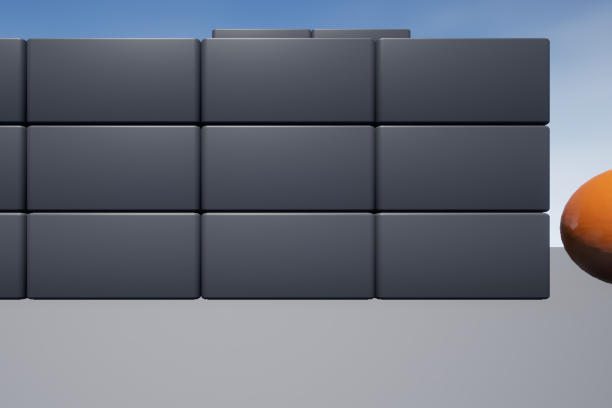
\includegraphics[width=0.3\columnwidth]{fig/check/airsim/block.png}}\quad
\subfloat[足球场]{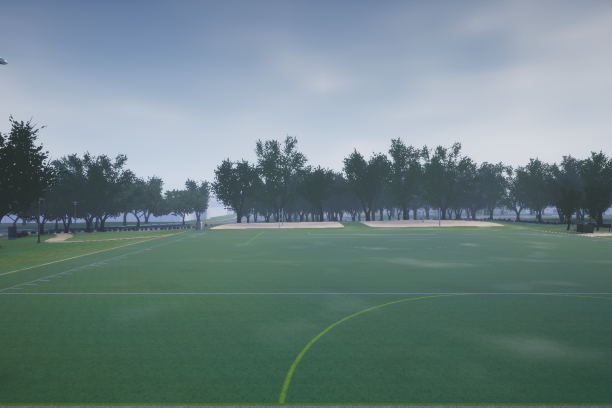
\includegraphics[width=0.3\columnwidth]{fig/check/airsim/ms.png}}\quad
\subfloat[废弃公园]{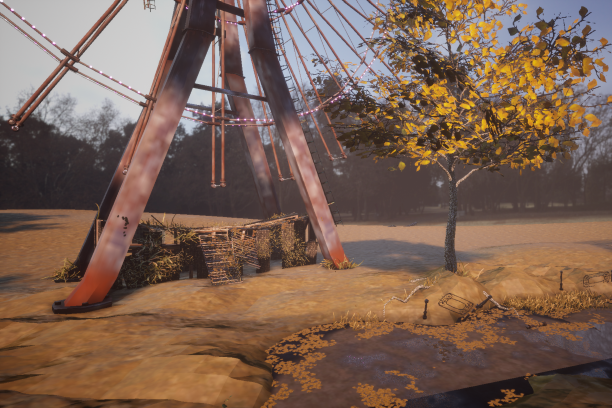
\includegraphics[width=0.3\columnwidth]{fig/check/airsim/park.png}}
}
\centering{
\subfloat[室内场景]{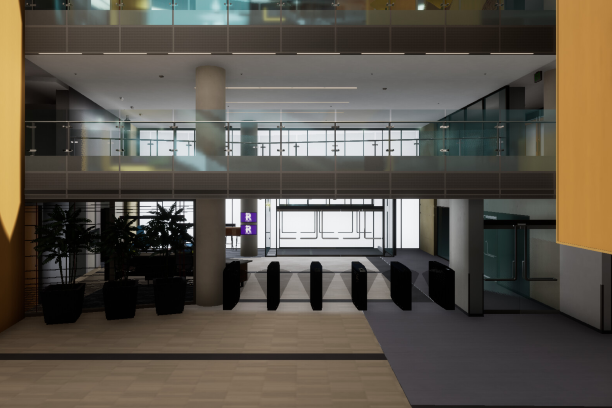
\includegraphics[width=0.3\columnwidth]{fig/check/airsim/building.png}}\quad
\subfloat[城市街区]{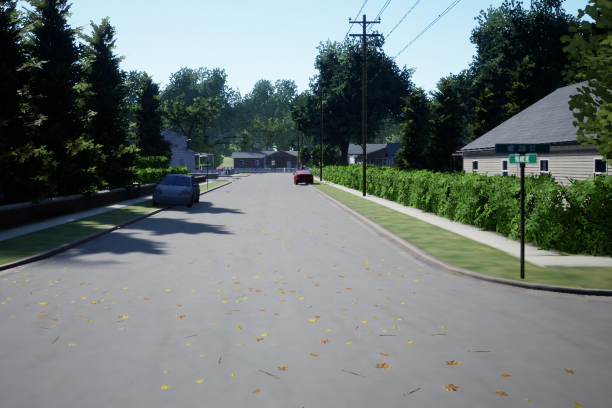
\includegraphics[width=0.3\columnwidth]{fig/check/airsim/neighborhood.png}}\quad
\subfloat[大型城市]{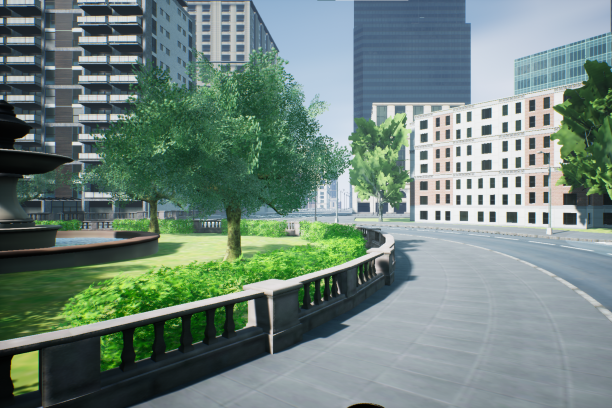
\includegraphics[width=0.3\columnwidth]{fig/check/airsim/city.png}}
}

\caption{Airsim中不同场景的模拟环境}
\label{fig:check_airsim} 
\end{figure}

其中常规和\emph{阵风晃动}实验在基本空间中进行,而\emph{轻微碰撞}实验则在所有六个模拟器环境中进行。
在进行常规和阵风晃动的飞行任务时,任务规划如图~\ref{fig:check_mission1}所示 (实线是实现的轨迹,虚线是计划的轨迹)。
每次任务的构成有图中的$16$个航点以随机的方式进行连接。
参考优秀商业无人机\tool{MavicPro2}~\footnote{\url{https://www.dji.com/hk-en/mavic-2?site=brandsite&from=nav}}的抗风能力,该产品能够抵抗六级风($8.0m/s \sim 10.7m/s$)。
因此,本次实验的阵风速度被定义在$8.0m/s$到$10.7m/s$之间,并持续时间为$1\sim3$秒。
对于碰撞任务,实验在虚拟环境中选择有更多障碍物空间的核心区域,以确保碰撞事件必须发生。
而在飞行过程中,如果发生了碰撞,但在三秒内没有出现落地的情况,实验就将其视为\emph{轻微碰撞}。
图~\ref{fig:check_mission2} 展示了两个有碰撞的飞行任务的例子,其中灰色物体是障碍物,橙色点是计划的飞行航点,绿色点是飞行起飞点,虚线是飞行任务路径,实线是无人机实现的路径,红色圆圈是碰撞痕迹。

\begin{figure}[htb]
\centering{
\subfloat[常规和阵风任务]{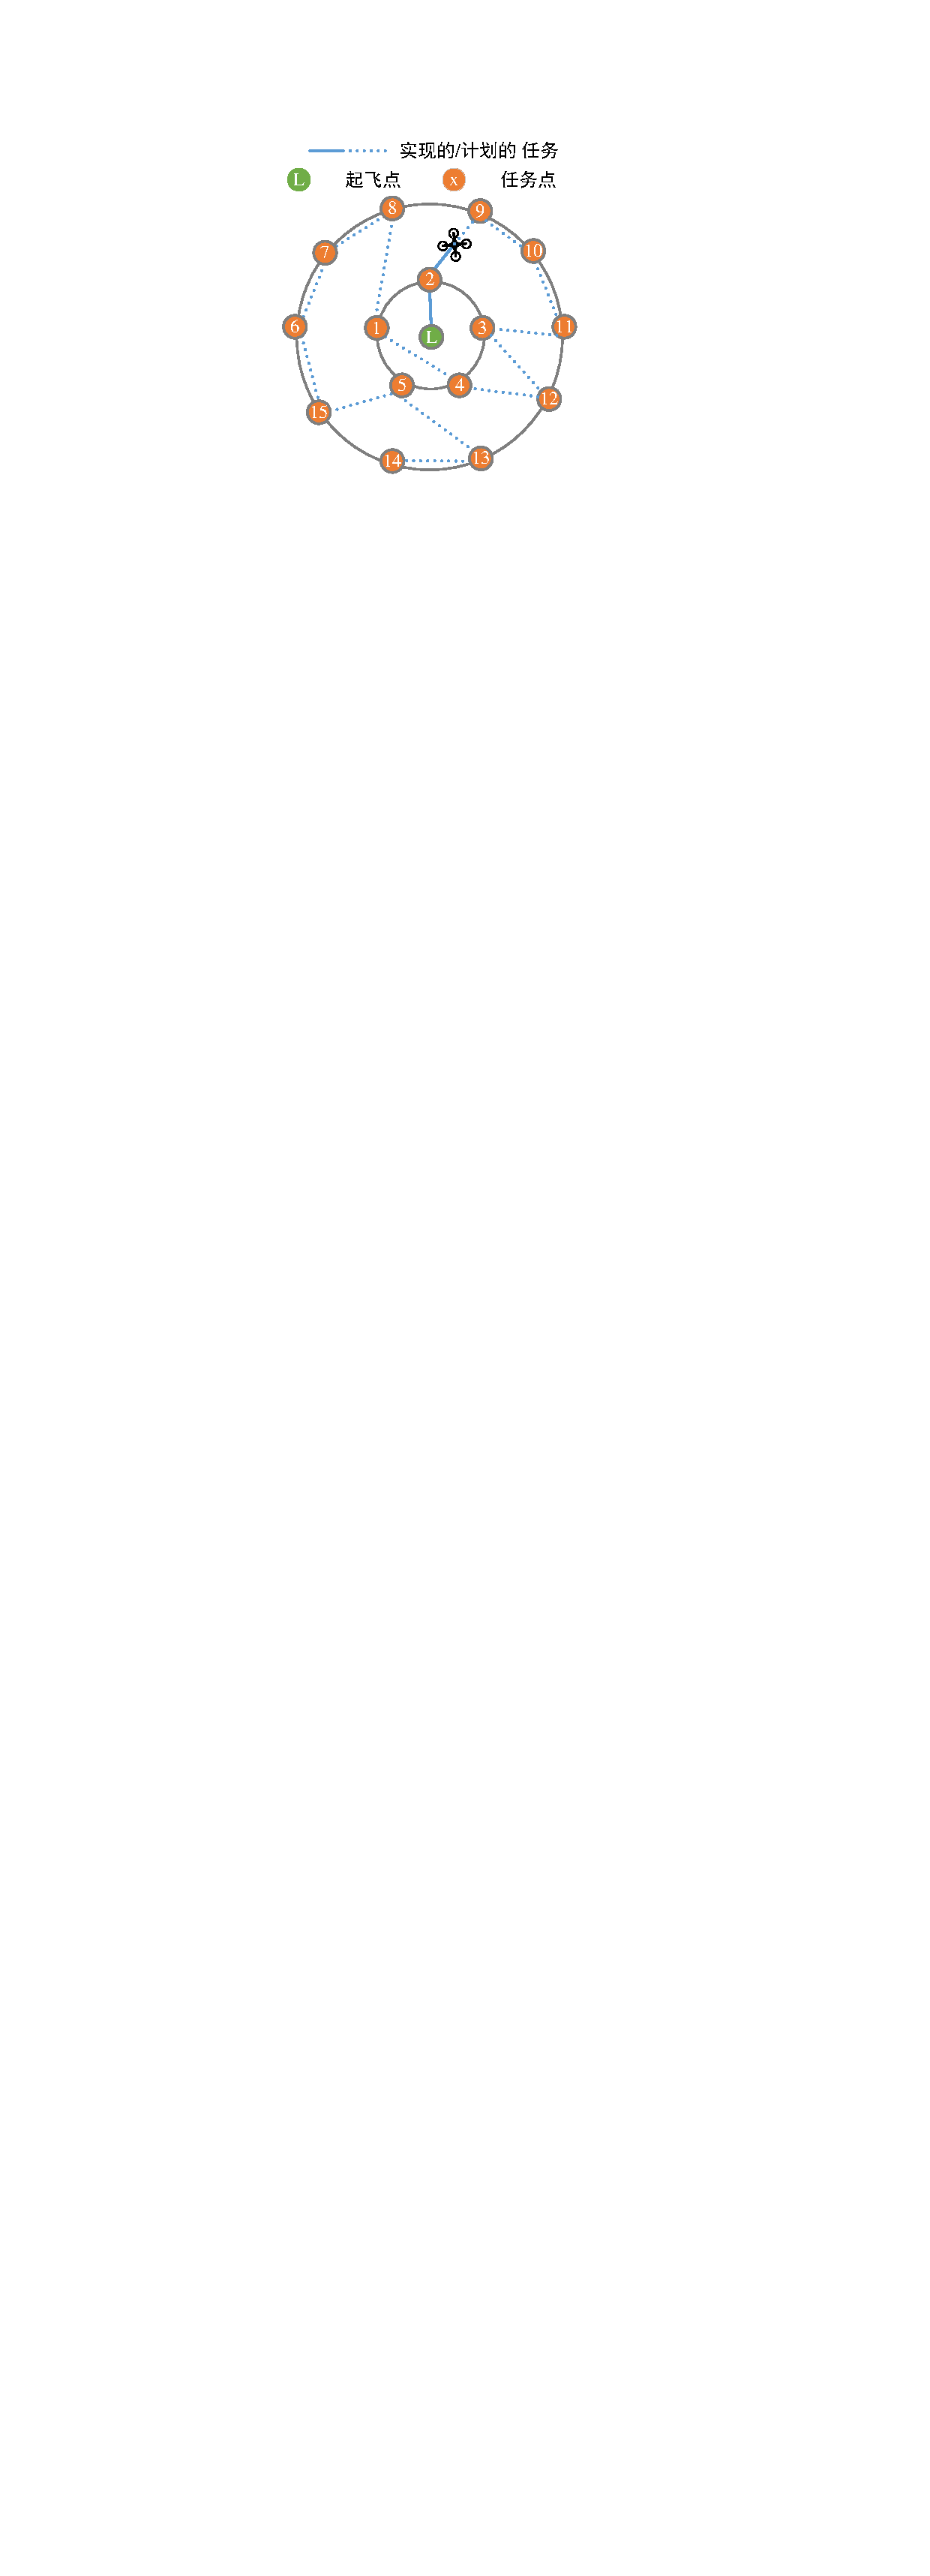
\includegraphics[width=0.35\columnwidth]{fig/check/ardupilot/mission.pdf}\label{fig:check_mission1} }
\subfloat[碰撞任务]{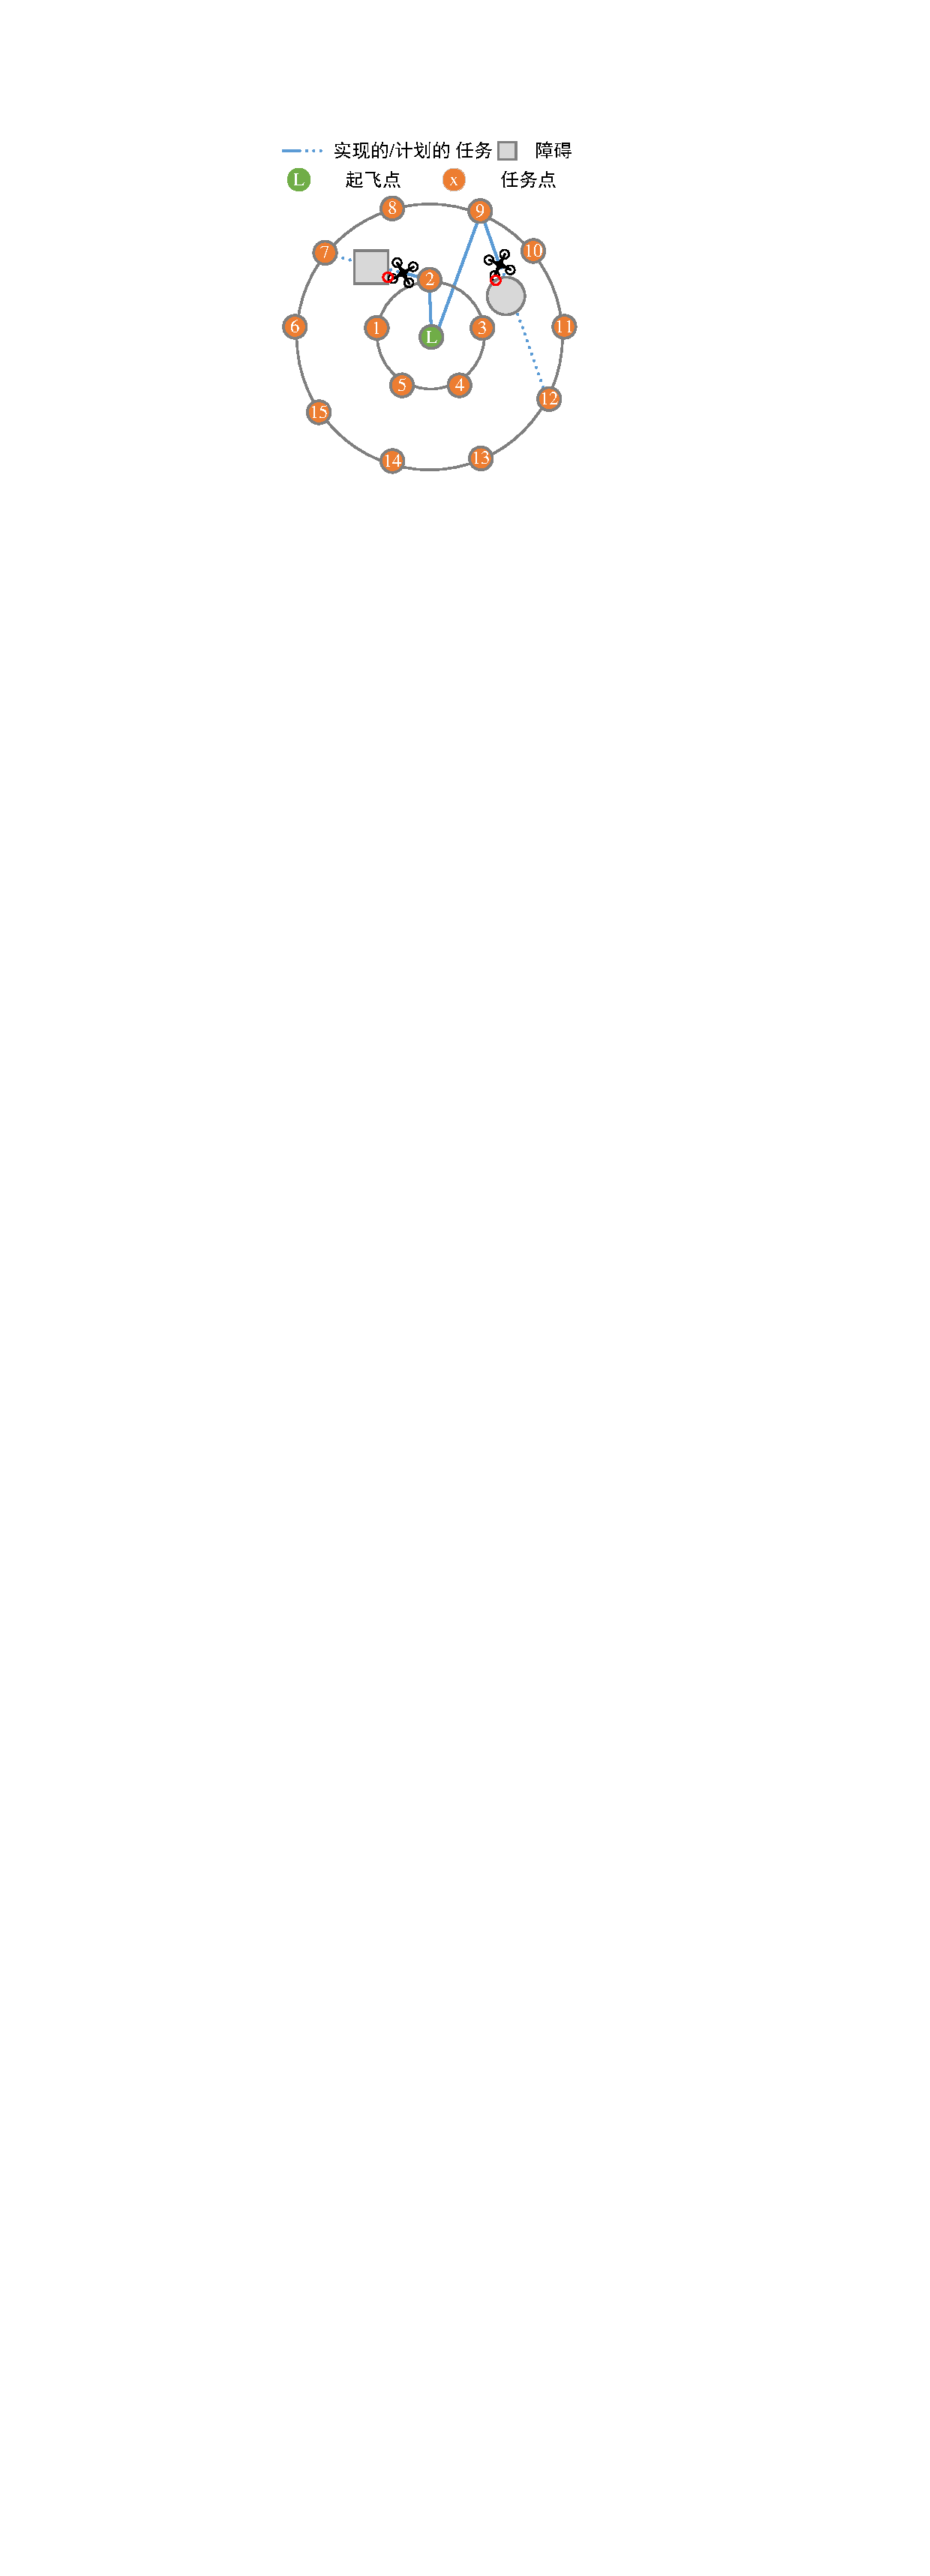
\includegraphics[width=0.35\columnwidth]{fig/check/ardupilot/mission2.pdf}\label{fig:check_mission2} }
}
\caption{飞行任务样例}
\label{fig:check_mission} 
\end{figure}

实验启动了$1,000$个常规飞行任务以产生飞行日志,并提取了$690,875$个飞行信息条目。
对于不安全事件检测的相关实验,实验启动了$1,000$个阵风实验,总共提取了$16,302$个信息条目;以及$1,000$个轻微碰撞实验,提取了$35,592$个信息条目。
为了进行比较,实验还选择了在章节~\ref{sec:check_problem}中描述的$100$个\emph{轻微碰撞}和$100$个\emph{阵风晃动}事件例子。


\subsection{提升评估标准}
由于系统的目标是处理\emph{不足事件}和避免由\emph{过度事件}引起的错误警报,安全检查的增强主要涉及两个指标,准确率(ACC)和假阳性率(FPR),定义如下。
\begin{equation}
    ACC = \frac{ TruePositive +  TrueNegative}{TotalPopulation}
\end{equation}

\begin{equation}
    FPR = \frac{FalsePositive}{ConditionNegative}
\end{equation}

其中$TruePositive$是正确识别的正例(即崩溃或推力损失)的数量。
    $TrueNegative$是正确识别的负例的数量。
    $TotalPopulation$是整个样本的数量。
    $FalsePositive$是被错误地标记为正例的样本数。
    $ConditionNegative$是被标记为负例的样本数量。
\deccheck 的目标是找到尽可能多的\emph{不足事件}(即增加ACC),并减少被错误地标记为正例的样本数量(即减少FPR)。


\subsection{研究问题1: 不变量有效性}
这个实验展示提取状态不变因素的过程,并验证了它可以有效地预测飞行状态的变化。
此外,本章节还评估了状态不变因素对环境风和飞行器模型的适应性。

\subsubsection{状态预测}
实验将$690,875$个收集到的数据分成$621,788$个用于训练状态不变量,剩下的$69,087$用于性能测试。
为了保证实验的真实性和可重复性,实验采用5折交叉验证法来记录不同输入$h$的平均准确率。
经过多轮的模型训练,不变量的预测性能如表~\ref{tab:check_cross}所示。
在不同的输入长度下,不变量的预测准确率都高于$98\%$,这说明不变量可以有效地预测参考状态,输入长度对预测的影响有限。
但为了得到最好的不变式以进一步建立特征,实验设定$h=2$,并选择性能最好的不变式模型进行后续实验。

\begin{table}[ht]
\caption{不同输入大小和测试数据集折叠的模型精度
}
\label{tab:check_cross}
\centering
\begin{tabular}{c|c|c|c|c|c|c}
        \toprule[1.5pt]
        输入长度  & 组1 & 组2 & 组3 & 组4 & 组5 & 平均 \\
      \midrule[0.8pt]
        1  & 0.9877 &	0.9877 &	0.9879 &	0.9881 &	0.9888 &	0.9880 \\
        
        2  & 0.9893 &	0.9903& 	0.9885 &	0.9914 &	0.9912& 	0.9901  \\
        
         3  & 0.9895 &	0.9898& 	0.9913 &	0.9904 &	0.9859 &	0.9894  \\
        
        4  & 0.9919 &	0.9874& 	0.9906& 	0.9916 &	0.9893 &	0.9901  \\
        
        5  & 0.9881 &	0.9901 &	0.9871 &	0.9892& 	0.9912 &	0.9891 \\
        \bottomrule[1.5pt]
\end{tabular}
\end{table}


\subsubsection{环境风适应性}
风是环境中最大的不确定因素。
实验进行了多次飞行任务以验证环境风是否影响了不变的预测。
实验分别发起$5$组飞行任务,每组包含$10$个飞行测试,每组的风速分别设置为$(0,1]$、$(1,2]$、$(2,3]$ 和 $(3,4]$ $m/s$。
测试将每组飞行实验的飞行数据条目输入到不变量当中来测试预测准确性,每组的平均结果如表~\ref{tab:check_wind}所示。
通过表可以观察到持续的风(不超过无人机性能的阈值)对不变预测的影响很小,平均准确度超过 $99\%$。
这是因为控制程序本身可以通过\tool{Kalman滤波}~\cite{vilez2015trajectory}来消除持续环境风的影响。
虽然一般的持续风对飞行影响不大,但是由于阵风震动具有持续时间短、风速大的特点,控制程序无法消除其影响,从而引发后续问题。
总体来讲,不变量模型不受持续正常风的影响,但可以有效地描述阵风的影响。

\begin{table}[ht]
\caption{不同风速下的模型精度}
\label{tab:check_wind}
\centering
\begin{tabular}{c|c|c|c|c}
        \toprule[1.5pt]
        风速级别(m/s) & \textbf{(0,1]} & \textbf{(1,2]} & \textbf{(2,3]} & \textbf{(3,4]}  \\
        \midrule[0.8pt]
        平均准确率  & 99.57\% & 99.49\% & 99.37\% & 99.17\% \\
        \bottomrule[1.5pt]
\end{tabular}
\end{table}

\subsubsection{飞行器适应性}
为了验证一个不变量是否具有普遍的适应性以应用到其他无人机飞行器模型上,测试实验使用不同的无人机设备测试状态不变量的预测准确性。
不变量从\tool{Airsim(ArduPilot)}无人机中提取,并将其应用于测试 \tool{Morse}、\tool{Gazebo}、真实无人机和 \tool{JMavsim} 的预测准确性。
具体方法为使用其他飞行器设备的飞行模型输入到不变量中来测试不变量的预测准确性。
表~\ref{tab:check_sim} 显示了不同车型的平均准确率。
从表中可以观察到,如果飞行器具有相同的控制程序(不论是模拟的还是现实的),状态不变量可以有效地预测它们状态的变化趋势,其准确度高于97\%。
但\tool{JMavsim (PX4)}这种具有飞行控制程序的表现结果较差。
这说明从某一特定飞行控制程序提取的不变量不适用于其他飞行控制程序,这是因为控制程序具有不同的状态估计逻辑和控制算法。
虽然如此,本方案依旧可以使用相同的流程来提取\tool{PX4}的状态不变量。


\begin{table}[ht]
\caption{不同车型的不变量预测准确性}
\label{tab:check_sim}
\centering
\begin{tabular}{c|c|c|c|c}
        \toprule[1.5pt]
        \multirow{2}{*}{车辆模型}&
        \multicolumn{3}{c|}{Ardupilot} & \multicolumn{1}{c}{PX4} \\
        
        \cmidrule[0.8pt]{2-5}
        
          & Gazebo & Morse & 真实无人机 & Jmavsim \\
        
         \midrule[0.8pt]
        
         准确率  & 97.30\% & 99.95\% & 99.87\% & 78.65\% \\
        
        \bottomrule[1.5pt]
\end{tabular}
\end{table}

\subsection{研究问题2: 检测性有效性}
此实验中主要验证了检测器的有效性,并选择了有代表性的样本来展示段不变差特征。

\subsubsection{有效性}  
实验首先使用状态不变量来生成不安全事件的特征,同时将特征作为数据集来训练检测器。
总体上讲,实验使用了$6,520$个常规飞行特征数据、$5,932$个\emph{轻微碰撞}特征数据、$2,717$个\emph{阵风晃动}特征数据,其中$5,868$常规飞行特征数据、$5,932$个\emph{轻微碰撞}特征数据、$2,717$个\emph{阵风晃动}特征数据用于训练分类器,其余的用于测试性能。
为了说明使用段不变差的必要性,作为比较,实验还训练了一个直接使用原始数据而不是段不变差特征的检测器。
两者都在测试数据中得到了验证,其性能如表~\ref{tab:cross_cnn}所示,其中\dquote{使用不变量}表示的是检测器应用段不变特征来训练的测试结果,而\dquote{不使用不变量}代表检测器直接使用原始段数据进行训练的结果。
从表中可以观察到,使用不变量的检测器具有更好的识别Precision,其F1-Score超过均$90\%$。
此外,与原始特征相比,使用不变量具有更平衡的Recall和F1-Score,也就是说,状态不变量对于复杂的不安全事件检测是有积极影响的。

\begin{table}[ht]
\caption{不同特征方式下物理安全事件检测的平均性能指标}
\label{tab:cross_cnn}
\centering
\begin{tabular}{c|c|ccc}
        \toprule[1.5pt]
        {特征} & {类别}  & {Precision} & {Recall} & {F1-Score}  \\
        \midrule[0.8pt]
        \multirow{3}{*}{使用不变量} & 轻微碰撞 & 98.20\% &   91.09\%  &  94.51\% \\
        
        & 正常飞行  & 92.02\%  &  99.58\%   & 95.65\% \\
        
        & 阵风晃动  & 97.38\%  &  86.67\% &   91.71\% \\
        \midrule[0.8pt]
        \multirow{3}{*}{不使用不变量} & 轻微碰撞 & 96.51\% &   92.48\%  &  94.45\% \\
        
        & 正常飞行  & 82.91\%  &  99.98\%   & 90.66\% \\
        
        & 阵风晃动  & 98.76\%  &  79.33\% &   87.99\% \\
        \bottomrule[1.5pt]
\end{tabular}
\end{table}

\subsubsection{不安全事件的特征案例}
本小节选择有代表性的事件数据样本段并展示使用不变量所生产的相应的特征。
图~\ref{fig:check_nnexample} 显示了\emph{轻微碰撞}和\emph{阵风晃动}的特征可视化值。
从图中可以清楚地观察到这两个事件样例都有清晰的异常值情况。
对于\emph{轻微碰撞}的例子,它标记了GPS故障、位置估计不良、故障安全和过度振动补偿激活的错误信息。
该事件影响了无人机的飞行状态,特别是Roll、Pitch和Pitch Rate。
至于\emph{阵风晃动}的例子,瞬时阵风会导致无人机向某个方向连续漂移,导致矩阵的某些列产生异常的持续。
两者之间的差异可以用分段不变的差异来清楚地描述。
图~\ref{fig:check_cov_kernal} 展示检测器识别这两个特征的热图,其中颜色深的部分表示这部分的数据在检测器识别中起到了较为主要的作用。
可以观察到,检测器的关注区域与实际产生差异的区域相近。


\begin{figure}[htb]
\centering{
\subfloat[
段不变差的示例,
颜色深浅表示原始值和预测值之间的偏差
]{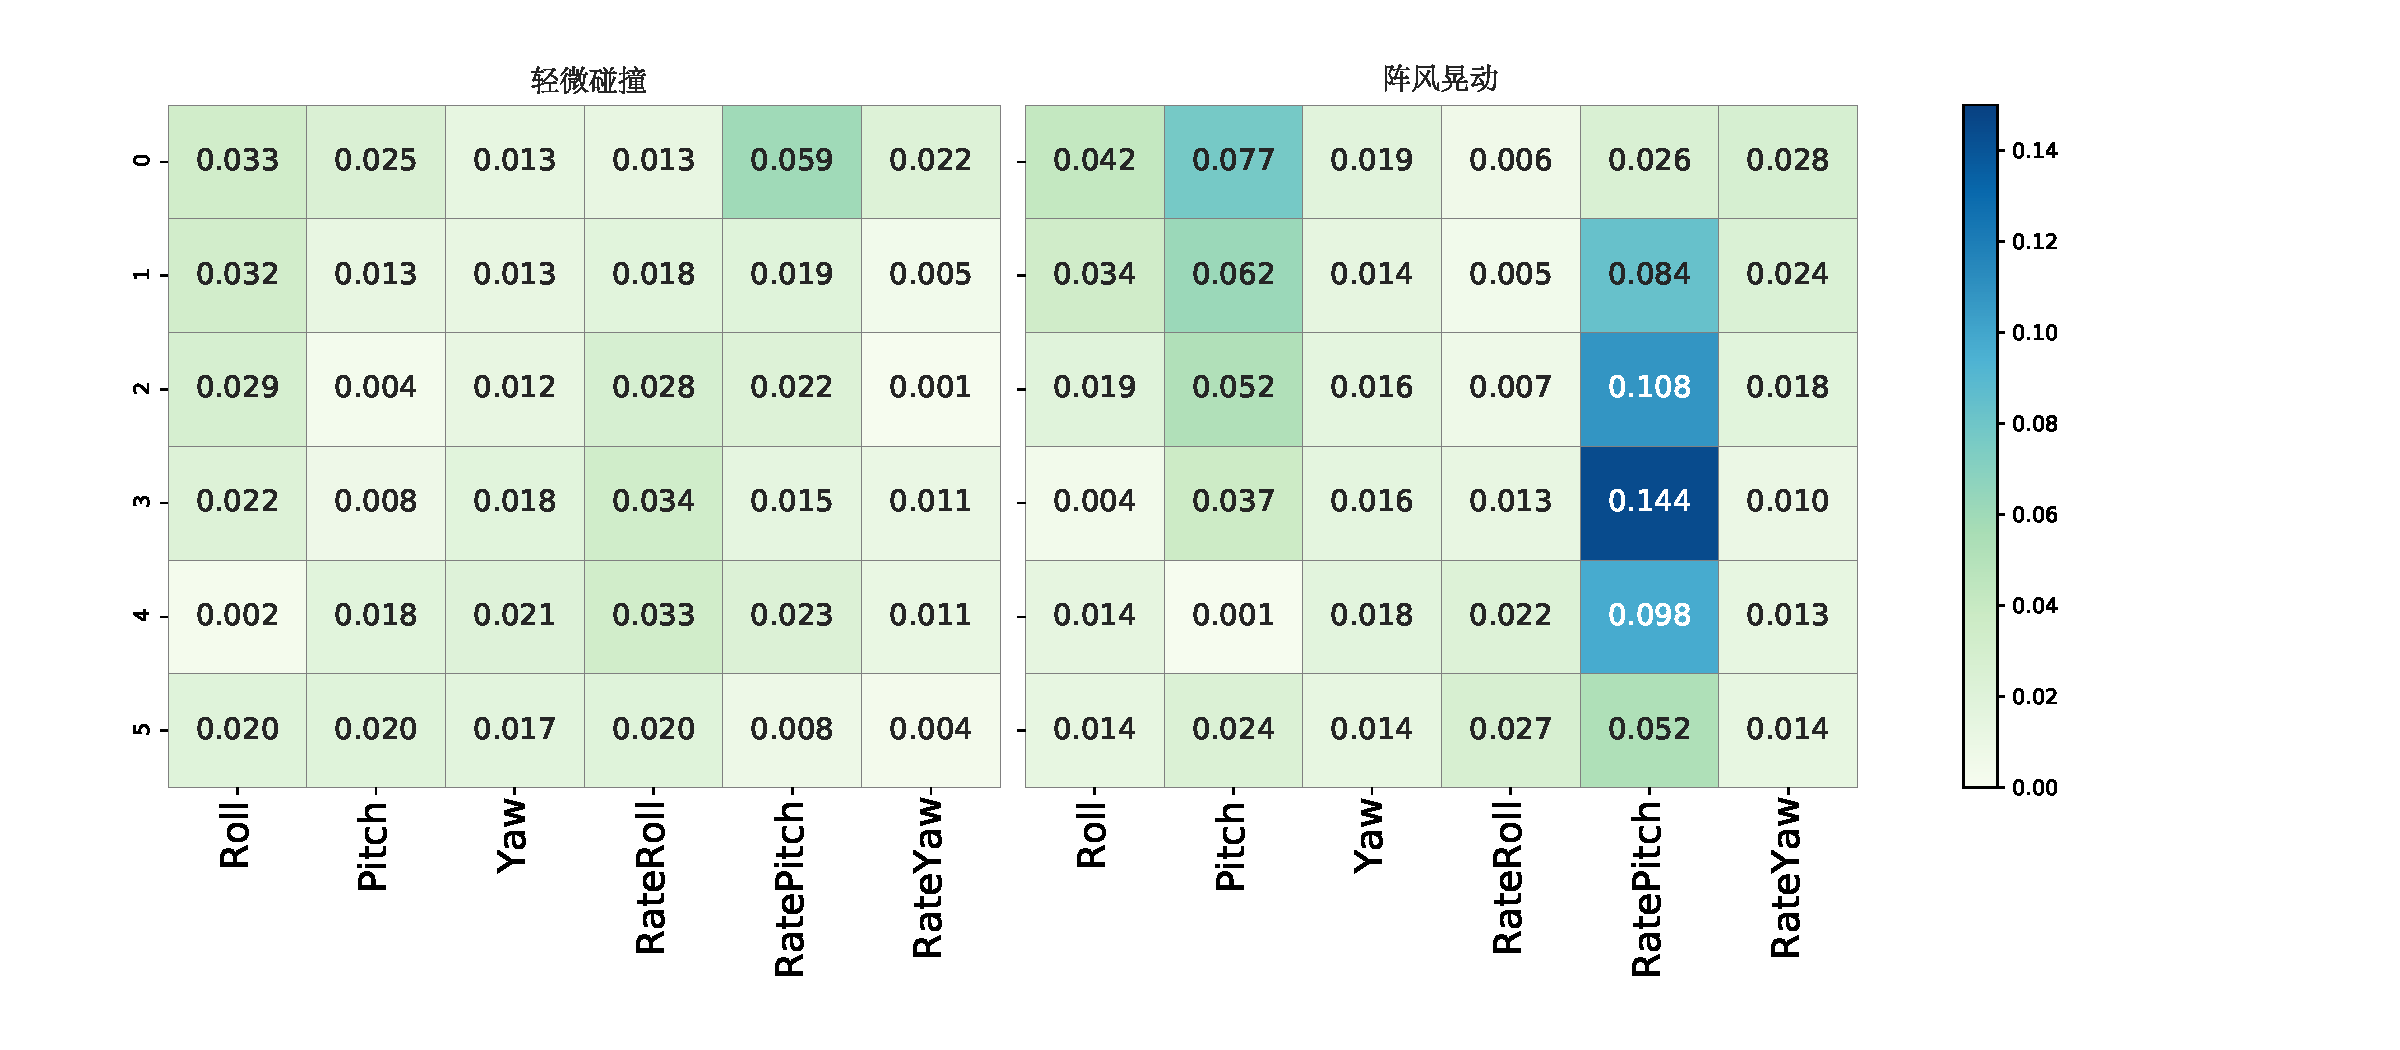
\includegraphics[width=\linewidth]{fig/check/nn/example.pdf}\label{fig:check_nnexample}}
\centering{
\subfloat[
检测器决策类别的热图,
颜色深浅表示分类的决策权重
]{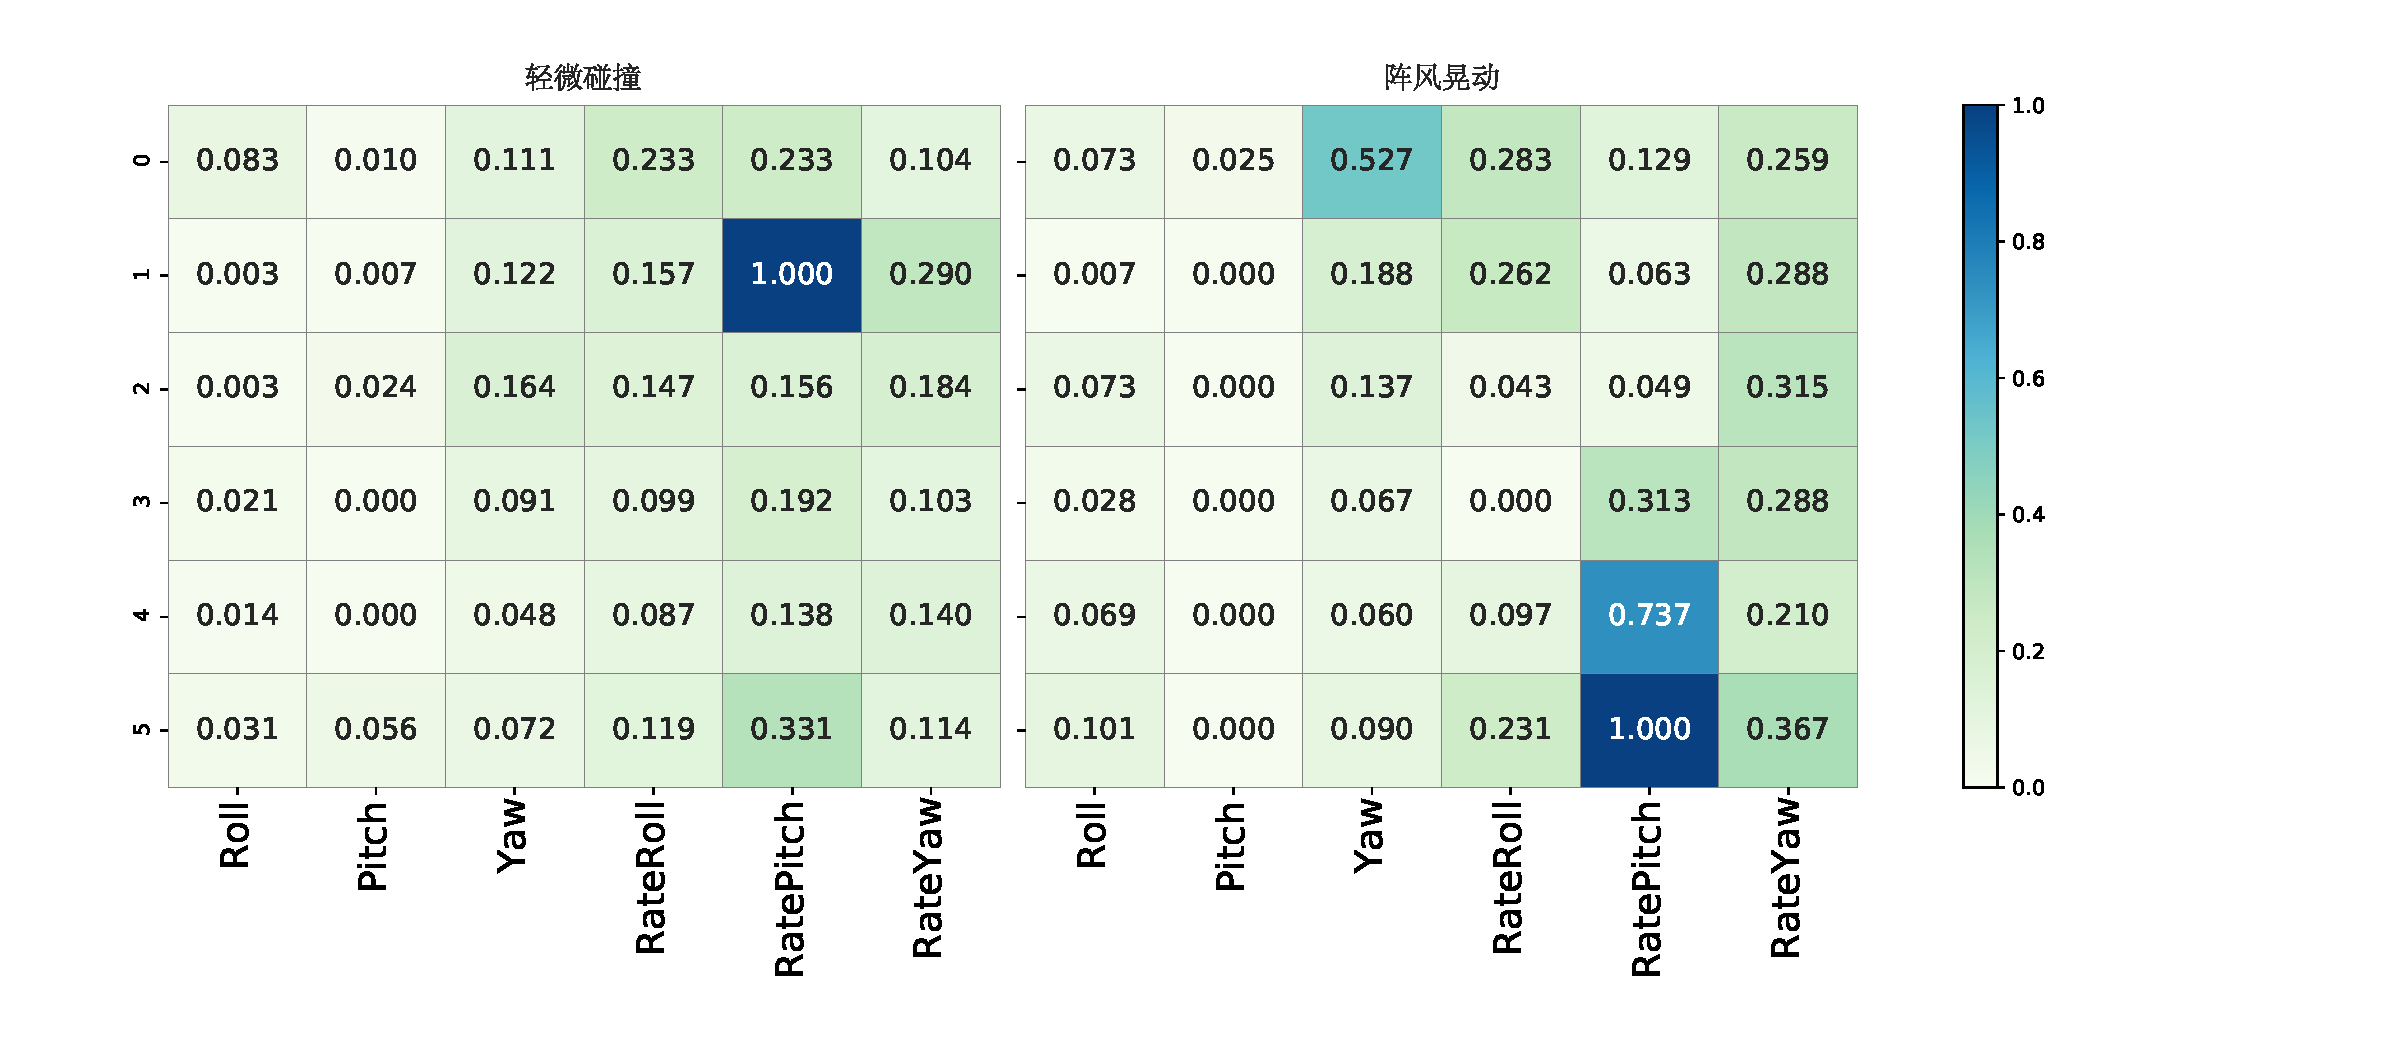
\includegraphics[width=\linewidth]{fig/check/nn/cov_example.pdf}\label{fig:check_cov_kernal}}
}
}
\caption{检测器决定热图样例} 
\end{figure}



\subsection{研究问题3: 效率与对比研究}
为了评估该系统是否能够提高处理复杂不安全事件的安全检查能力,此实验主要与原始安全检查系统进行了比较。
同时,为了显示其优势,本节实验还将其与其他较新的的异常检测方法进行了比较,这些方法包含\tool{SSR}~\cite{choi2020software}和\tool{PID-Piper}~\cite{piper}。
\tool{SSR}是一个用于飞行器的恢复框架,它通过线性模型预测来验证异常值并从不安全状态中恢复。
\tool{PID-Piper}是一个新颖的机器人飞行器的异常检测和飞行恢复系统,它应用非线性学习模型来实现与\tool{SSR}相同的功能。
需要注意的是,两者都有检测和恢复阶段,但在本实验只利用其异常检测阶段进行比较。

\subsubsection{功能提升}
实验使用与章节~\ref{sec:check_problem} 中一致的离线日志数据进行实验。
实验内容为使用\deccheck 去检查此前的飞行日志,看是否会触发其功能。
表~\ref{tab:check_cmp_check} 展示了\deccheck 的反应,其中\dquote{识别}表示\deccheck 识别的事件数,\dquote{辅助检查}代表安全检查的辅助修正。
原来的安全检查(见表~\ref{tab:check_crash_err})只识别出$2$个\emph{轻微碰撞},但实际上发生了$100$起\emph{轻微碰撞},而其汇报的$44$个推力损失信息均为误报。
与系统原始的安全检查相比,\deccheck 检测到 $81$\emph{轻微碰撞}和$76$\emph{阵风晃动}事件。
它补充了$79$ 碰撞警告并减少了$44$推力损失误报中的$36$个,这将碰撞检查的的ACC 从$2\%$ 增加到$81\%$,将推力损失检查的FPR 从$44\%$ 减少到$6\%$。

尽管\deccheck 可能会错误地检测到不安全事件(例如,将阵风震动报告为碰撞),但它不会对无人机造成致命后果,因为最终辅助判断是结合了原始安全检查和\deccheck 识别的。
由于安全检查没有推力损失警告,因此识别碰撞的假阵风震动检测不会生效。
至于识别阵风晃动时误判坠机,只会触发降落或返回操作,不会导致额外的威胁。

\begin{table}[ht]
\caption{\deccheck 对于安全检查的加强}
\label{tab:check_cmp_check}
\centering
\begin{tabular}{c|c|c|c}
        \toprule[1.5pt]
         {事件}  & {识别} & {辅助检查} & {修正} \\
         \midrule[0.8pt]
         轻微碰撞 & 81 & 碰撞检查 + 79  &  ACC: $2\% \to 81\%$\\
        阵风摇晃 & 76 & 动力损失误报 - 36 &  FPR : $44\% \to 6\% $ \\
        \bottomrule[1.5pt]
\end{tabular}
\end{table}
 

下面演示一个\deccheck 协助安全检查的例子。
实验进行了三个任务相同的飞行:常规飞行、阵风晃动飞行、阵风晃动但是装备了\deccheck 。
图~\ref{fig:check_pedec_work} 演示轨迹对比,其中红点为飞行轨迹点,白线为任务轨迹。
在常规飞行情况下(图~\ref{fig:check_dec_regular}),无人机可以右转并继续执行任务。
\emph{阵风晃动}事件会触发推力损失并启动电机助力,从而导致偏差(图~\ref{fig:check_dec_gust})。
在\deccheck 的帮助下,虽然安全检查发出了推力损失警告,\deccheck 确认这是\emph{阵风晃动}并中断了进一步的电机助力以保持正常飞行(图 ~\ref{fig:check_dec_pedec})。

\begin{figure}[htb]
\centering{
\subfloat[常规飞行]{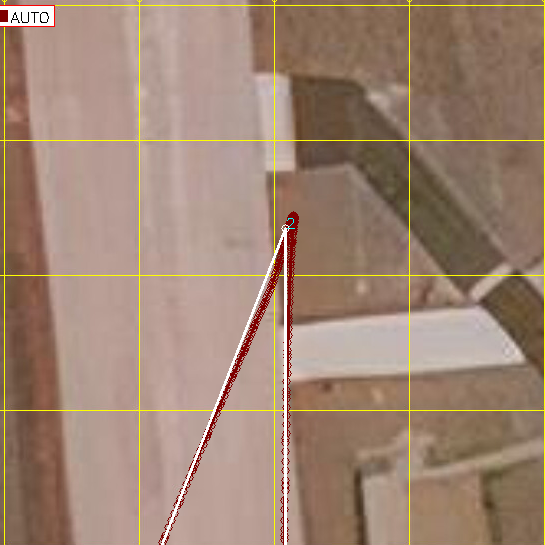
\includegraphics[width=0.32\columnwidth]{fig/check/cmp/regular.png}\label{fig:check_dec_regular} }
\subfloat[阵风晃动]{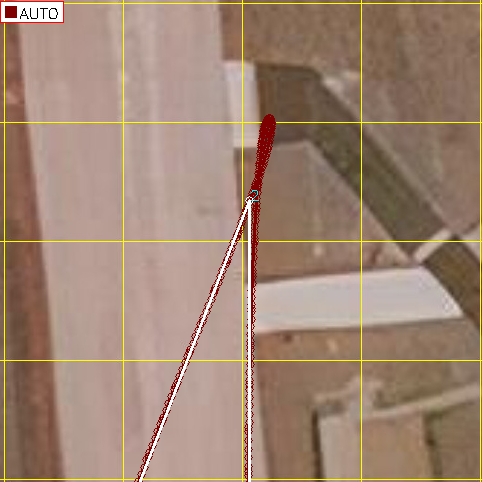
\includegraphics[width=0.32\columnwidth]{fig/check/cmp/gust.png}\label{fig:check_dec_gust} }
\subfloat[\deccheck]{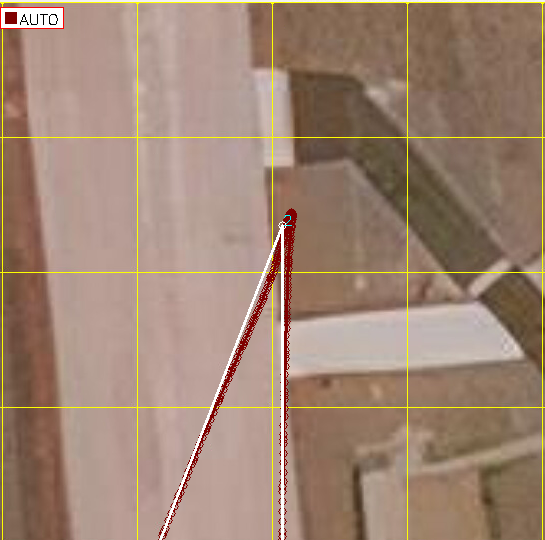
\includegraphics[width=0.32\columnwidth]{fig/check/cmp/pedec.png}\label{fig:check_dec_pedec} }
}
\caption{三种情况的飞行轨迹}
\label{fig:check_pedec_work} 
\end{figure}

\subsubsection{研究对比}  
对比研究使用相同的实验方法($100$ \emph{轻微碰撞}和 $100$ \emph{阵风晃动}事件)来展示三个系统的检测结果:\deccheck 、\tool{SSR} 和 \tool{PID-Piper}。
\deccheck 在不变量和检测器中使用最佳性能模型。
由于SSR不是公开可用的,此处实验使用其文章中公布的架构来实现相同的功能,识别但使用本实验相同的常规数据来进行训练。
对于 \tool{PID-Piper},参考源代码~\footnote{\url{https://github.com/DependableSystemsLab/pid-piper}}并使用本次实验的常规数据实现相同的架构模型。

\begin{figure}[ht]
  \centering
    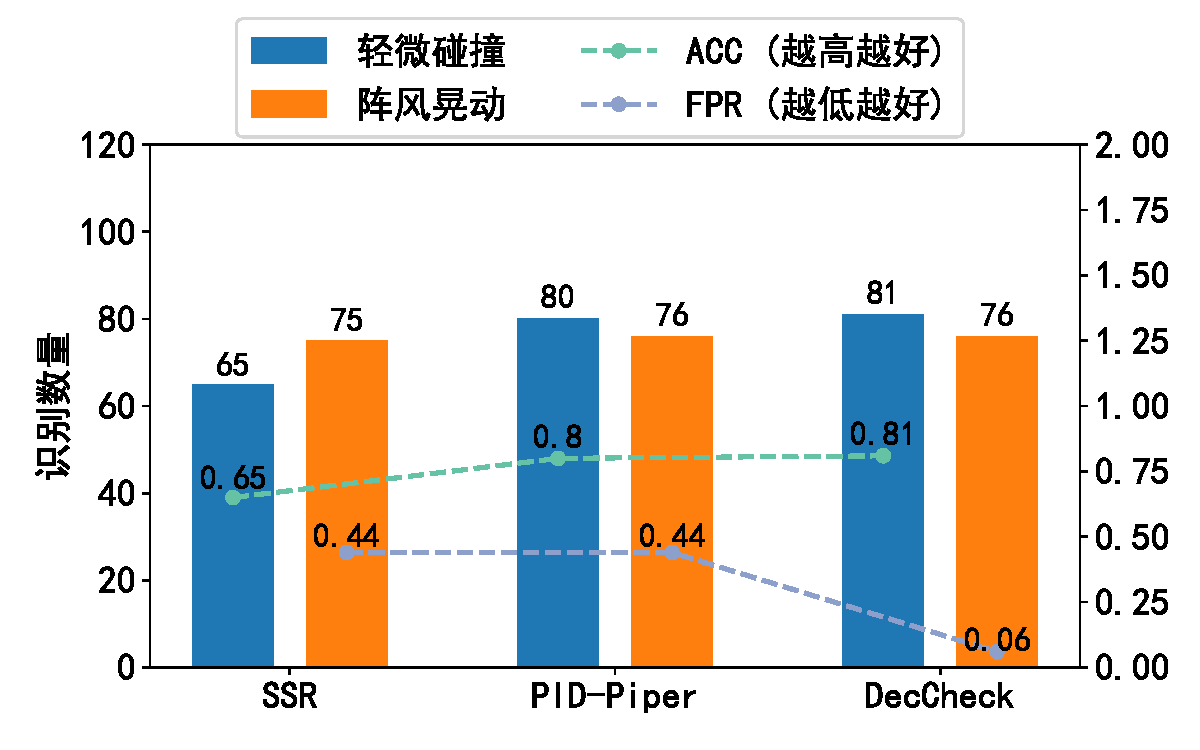
\includegraphics[width=\columnwidth]{fig/check/cmp/cmp.pdf}
\caption{\tool{SSR}、\tool{PID-Piper}和\deccheck 对物理事件的处理结果}
\label{fig:check_cmp} 
\end{figure}  

图~\ref{fig:check_cmp} 揭示了三个解决方案对于两种不同物理不安全事件的反应。
对于\tool{SSR} 和\tool{PID-Piper},他们分别检测到$65$个和$80$个\emph{轻微碰撞};
分别检测到$75$和$76$个\emph{阵风晃动}事件。
\deccheck 检测到 $81$ 个\emph{轻崩碰撞}和 $76$ 个\emph{阵风晃动}事件。
如果只评估异常检测结果,\deccheck 和 \tool{PID-Piper} 的性能优于最较早早提出的 \tool{SSR}。
因为无人机在其状态值之间具有非线性关系,因此线性方法 \tool{SSR} 可能会失去检测准确性。
但是如果考虑 ACC 和 FPR 的增强,\deccheck 具有最好的性能,它具有最高的 ACC,同时保持最小的 FPR。
这是因为 \tool{SSR} 和 \tool{PID-Piper} 只考虑异常检测而没有识别它们的类型。
它们采用相同的策略来处理不同的异常状态,这不适用于复杂的不安全事件。
虽然它们可以帮助系统安全检查增强\emph{轻微碰撞}检测的能力(提高 ACC),但它们不能降低推力损失的 FPR,这仍然会报告由\emph{阵风晃动}事件引起的异常反应。


\subsection{系统消耗}
在服务器训练阶段,LSTM需要$707.68$秒时间,CNN需要$23.87$秒的时间来优化学习模型直到达到收敛。
在检测阶段,根据飞行取样数据,Raspberry Pi 4B产生$10,000$的分段预测实例耗时$3.978$秒,验证$10,000$个的实例耗时$1.971$秒。
综上所述,机载计算机能够以合理的采样间隔有效地进行物理飞行事件的异步验证。

\section{本章小结}
本小节介绍了由于复杂的物理事件而导致的无人机安全检查系统出现错误反应的情况。
\emph{不足事件}不足事件会使得无人机安全检查系统无法正确的检出这类危险事件,从而导致系统错误判断自身问题并进一步造成安全问题。
\emph{过度事件}则是错误的引发了无人机安全检查系统的响应,但是这种错误的相应反而中断了无人机的正常飞行。
本小节通过\deccheck ,一个应用状态不变和机器学习检测器的系统来解决上述事件造成的问题。
\deccheck 建立的环境来收集各种事件数据,利用神经网络提取飞行状态不变量,最后应用不变量为每个事件创建相应的不变差异特征,并训练 CNN 模型来检测它们。
完备的实验证明也说明了\deccheck 系统在帮助无人机抵御这种复杂的事件上面有较大的提升。





\chapter{模型预测的可靠参数配置方案}
\section{引言}
电子和传感器技术的进步拓宽了无人机的应用范围~\cite{bekmezci2013flying, bok2011context}包括但不限于交通监控、野外救援、商业快递和遥感等方面。
由于飞行场景的复杂性和不可控性,大多数飞行控制程序(如:\tool{PX4}~\cite{px4}、\tool{LibrePilot}~\cite{Librepilot}和\tool{ArduPilot}~\cite{ardupilot})都实现了一种动态调整机制,即参数配置。
这种参数配置机制可以让使用者或者开发者根据自身需求来平衡无人机的的可靠性(保持稳定飞行)和适应性(适用于更多场景)。
这种参数配置机制提供了大量的可调整参数来适应飞行硬件和任务的差异,例如可以调整无人机飞行的姿态的增益参数,电机的最大转速,任务飞行允许最大的倾角。
一个可靠而灵活的控制程序包含了数百个影响飞行行为的飞行参数。

然而,这些配置的安全性是不可预测的,因此在没有提前飞行测试的情况下,一些不适当的配置可能会被上传到无人机中,从而导致无人机做出不可逆的不稳定飞行。
例如,它会造成无人机实际的飞行轨迹偏离其预先规划的路径从而导致轨迹偏离,或者由于姿态异常导致电机无法提供更多的动力来维持飞行并进一步出现飞行推力损失警告,甚至这些配置可能会直接导致无人机坠毁。
为了维护配置的安全性和可靠性,控制程序的开发者或制造商提供了参数值选择的建议范围,以防止像这些不稳定的飞行那样的不可预测的事件发生。
虽然开发者在上尝试在安全配置方面做出了一定的防御机制,但由于缺乏对参数值的充分检查,这种范围限制机制仍然暴露出\textit{范围规范错误(Range Specification Bugs})。
具体来说,即使一些特定的配置中的参数值均在范围建议内,仍然可能被触发一些不稳定的飞行,即官方建议不能防止配置驱动无人机进入不稳定的飞行。

不幸的是,现有的无人机漏洞检测技术并不以检测/搜索这种漏洞为目的。
污点分析~\cite{cheng2018dtaint, she2020neutaint, chibotaru2019scalable, halin2019test}跟踪参数数据流以定位它对系统的影响。
然而,当处理非常多的控制参数时,每个参数都有很大的取值范围,测试覆盖所有的值是很耗时的。
此外,这种跟踪是在程序运行时进行的,这意味着对问题的定位需要进行无人机飞行任务测试来完成。
相关先进研究\tool{RVFuzzing}~\cite{rvfuzzer}使用模糊测试的方法来发现这种配置从而解决这样的问题。
尽管\tool{RVFuzzing}提出了两种二进制搜索方法来模糊测试配置的数量,但它仍然无法实现高覆盖率,并错过了一些包含不正确配置的搜索空间。
\tool{LGDFuzzer}~\cite{han2022control}采用了一种带有学习模型的模糊测试来评估配置,以加速搜索过程。
然而,该工作中的评估只考虑一个时间戳的预测偏差,这使得搜索结果很可能受到瞬时干扰的影响,影响搜索的准确性。

本章节提出一种新的基于模型预测的可靠参数配置方案,并实现了原型工具\icsearcher,一种带有预测器的模糊方法,它能够搜索不正确的配置并提供较为合理的范围指导以减少\textit{范围实现错误}出现的可能性。
整体上讲,\icsearcher 依赖于遗传算法(Genetic Algorithm,GA)~\cite{ga}和飞行状态预测器来检测潜在的不正确配置并从范围指南中剔除。 
具体来说,\icsearcher 由三个模块组成,即参考状态预测器、不正确搜索器和灵活的范围指南。
该方案首先通过手动收集飞行日志来创建生成预测器所需的数据,数据中的每个条目都包含飞行状态、传感器数据、配置和时间戳。
随后,\icsearcher 使用这些数据生成一个预测器,并使用它来估计一段一个无人机飞行的下一时刻的参考状态。
\icsearcher 的核心在于使用GA进行模糊搜索,从而找到潜在的不正确配置,这些配置被预测器评估为可能会导致无人机不稳定。
与传统的模糊验证方案,即通过现实或模拟执行来测试候选者不同,\icsearcher 用该预测器替代了GA中的反馈评估,即使用概率预测结果来驱动模糊搜索。
最后,\icsearcher 验证了被预测为\dquote{不正确}的配置,并根据这些验证结果进一步生成了灵活的参数范围。

\section{参数范围实现错误}
制造商提供由数百个参数组成的可配置控制方案,以支持各种飞行任务。
每个用户或者控制端可以通过调整这些参数值来控制无人机,以应对不同的任务场景。
然而,一些数值组合可能会导致不稳定的状态。
因此,控制系统的制造商同时提供了一种范围控制机制,通过每个参数的预设值范围指导参数选择。
以前的研究表明,这样的范围控制机制不能防止引入不正确的配置,即使是从预设范围内选择有效的参数值。
这些不正确的配置所造成的问题被称为\textit{范围规范错误(Range Specification Bugs)}~\cite{rvfuzzer, han2022control}。
这些配置会导致不稳定的飞行状态,并可能导致轨迹偏差和坠机等严重事故。
范围规范的错误从两个方面威胁着无人机,即外部攻击和内部误配置(如图~\ref{fig:range_attack}所示)。
\begin{itemize}

 \item \textbf{内部误配置:}
无人机的管理人员或内部人员,不熟悉配置无人机的正确方法,错误地配置了不适当的参数值。
不正确的配置会导致异常的飞行预期,由于缺乏准备知识,用户无法确定问题的根本原因。

\item \textbf{外部攻击:}假设攻击者通过模拟测试模拟无效的配置,可以利用无线/无线电通信的漏洞~\cite{kwon2018empirical,rodday2016exploring, vanhoef2017key}。
在没有任何恶意代码注入、内存损坏或传感器欺骗的情况下,攻击者构建并通过脆弱的无线/无线电通道向无人机发送了一连串的命令。
通过秘密地不正确的些配置发送给无人机,从而触发不稳定的物理状态并中断飞行任务。
为什么攻击者要费心去修改配置,而不是直接让无人机崩溃呢?
一个关键的考虑因素是这些攻击侧重于利用协议中的漏洞,而不是针对飞行系统,这意味着它们可以在不依赖代码注入或固件修改的情况下实现其目标。
需要注意的是,由于没有物理接触,攻击者无法轻易通过操纵控制程序来破坏或控制无人机。 
相反,这些协议充当用户和无人机之间的主要通信渠道,使它们成为潜在攻击的主要入口点。
与常规的用于进行攻击的恶意命令不同的是,不正确配置攻击利用的是无人机系统自身的逻辑设计缺陷而不是外部系统入侵。
而最近的研究~\cite{schiller2023drone}使用协议反向的方法将无人机的内部命令发送给DJI无人机,从而导致无人机重新连接。
这凸显了伪造命令和利用系统中的逻辑漏洞(例如范围规范错误)可能是攻击者的有效方法。 此外,此类攻击的优点是利用本机机制掩盖攻击者的意图,从而可能混淆后续的事故调查。



\end{itemize}

\begin{figure}[ht]
  \centering
    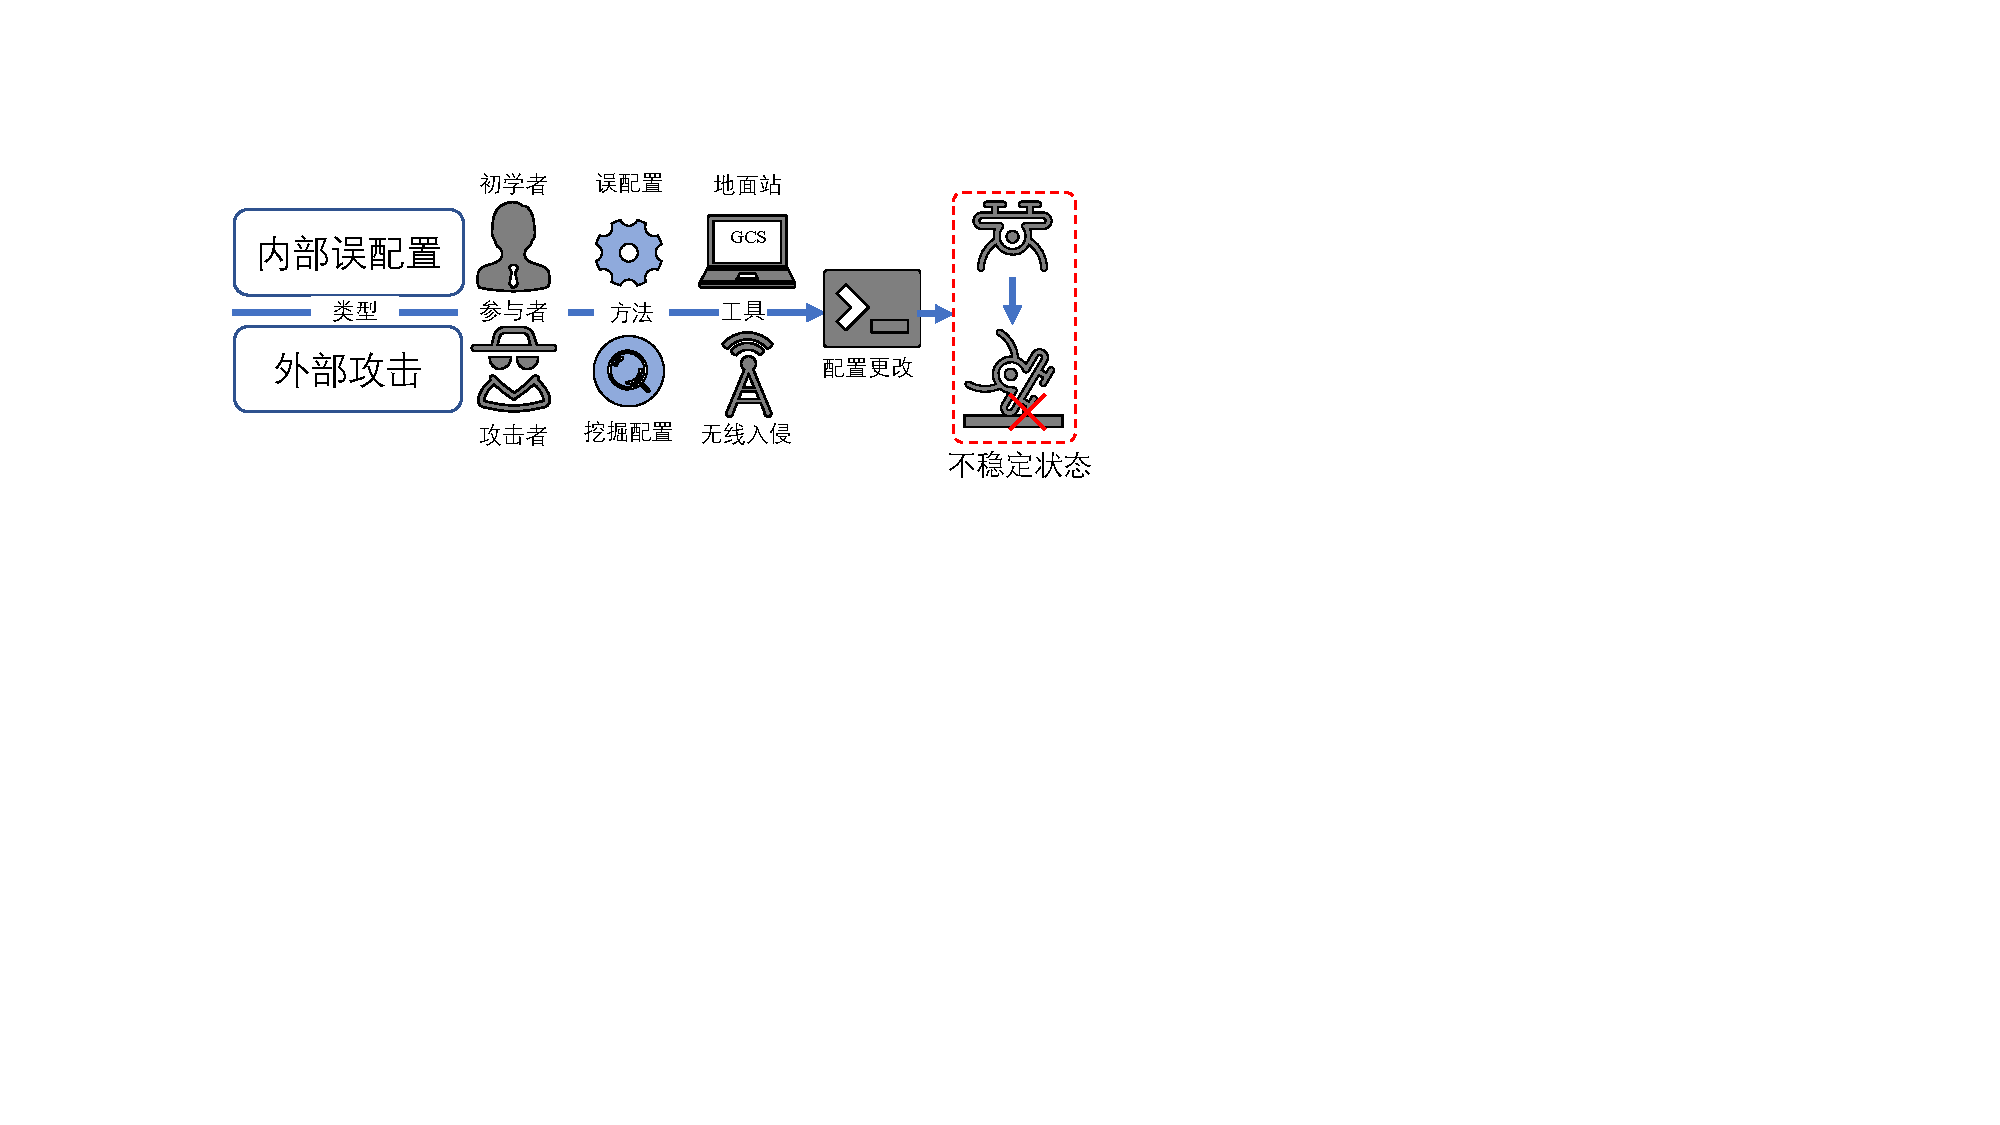
\includegraphics[width=0.9\columnwidth]{fig/background/attack.pdf}
\caption{两种情景下的威胁模型}
\label{fig:range_attack}  
\end{figure}


通常情况下,不正确的配置会导致无人机出现各种物理或系统问题。
通过飞行过程中的表现,\textit{范围实现错误}中的不正确的配置的影响可以归为以下几种情况:
\begin{enumerate}
    \item \textbf{飞行冻结:} 除非无人机正在执行降落或者悬停动作,一个正常的无人机飞行过程应该时刻保持着移动。
    然而,\textit{范围实现错误}中所出现的不正确配置可能会导致无人机在前进/后退时意外地冻结在一个航点上,或者在最小移动范围内的某个位置徘徊。
    
    \item \textbf{轨迹偏航:} \textit{范围实现错误}中的不正确的配置可能会影响无人机的飞行操控,引发重大的位置偏差。  
    这种偏差可能会导致错误的轨迹,无人机无法从中返回到正确的轨迹。
    
    \item \textbf{飞行坠毁:} 对于较小的飞行偏差,即使不是在预期的位置,无人机仍然可以安全降落。
    更糟糕的情况是,偏离导致无人机撞上一个物体,最终坠毁。

    \item \textbf{潜在动力损失:} 控制程序发送电机动力信号,驱动无人机飞行。通过调整转速从而调整其飞行姿态。
    然而,无人机电机所能做的调整是有限的。
    如果设置了\textit{范围实现错误}中的不正确配置,即使当前的油门已经使电机转速饱和到100\%,无人机控制算法仍然计算出需要更多的转速来保持飞行平衡。
    无人机持续保持这种需求状态会导致无人机飞行高度下降,甚至坠毁。

    \item \textbf{启动后的特权升级:} 在起飞前,飞行控制程序会验证配置以确定其在控制算法中的合理性。
    当发现一个或多个不正确的配置参数时,控制程序会显示一个警告信息并中止起飞操作。
    然而,如果这些被标记为不正确的配置是在起飞后被设置的,则仍然可以被飞行控制程序所接受,从而造成一系列的偏航,动力损失等后果。
\end{enumerate}

\section{挑战与解决思路}

\subsection{问题难点及挑战}
为了验证所有的配置和检测范围规范的错误,必须解决以下挑战。

\begin{itemize}
    \item \textbf{挑战 1: 如何有效地验证配置?}
先前所提出的分析飞行控制程序的方法一般是基于静态程序分析技术,他们主要搜索控制和数据的依赖关系~\cite{mayday,Believing,zhu2019new}。
然而,这种技术并不适合验证配置,因为需要分析大量的指定参数值。
传统静态分析方法只关心片段的代码,而无人机的这种配置问题需要分析整个飞行控制程序。
因为不同的参数值往往会导致涉及控制程序非常不同部分的执行流程,为了达到高代码覆盖率,若采用静态分析方法,只能对整个系统代码进行分析。
但是飞行控制程序具有巨大的代码规模(超过70万行的代码)和复杂的控制和数据依赖关系。
因此,为配置验证设计的方法必须是有效的,能够提供较高的测试覆盖率。

    \item \textbf{挑战 2: 如何高效地验证配置?}
一个配置的验证方式需要通过现实的或模拟的飞行执行进行测试。
但是由于控制参数的数量很多,每个参数的取值范围也很大。
改变参数值来生成配置并验证所有这些配置的效率很低。
维度爆炸和参数之间复杂的关联性进一步加剧了覆盖所有可能的参数组合的难度。
完成整个验证程序需要花费多至数十个小时。
因此,使用现有的方法~\cite{tartler,halin2019test}分析所有可能的配置并不适合。
另一种方法是使用模糊处理~\cite{rvfuzzer}结合二进制搜索~\cite{knuth1971optimum}来减少要分析的组合的搜索空间。
然而,该方法虽然尝试缩小搜索范围,但是由于算法本身设计的问题,无法进行多线程验证。
因此每个模糊分析迭代都需要等待,直到获得前一个配置的验证反馈。这大大增加了搜索的时间成本。


    \item \textbf{挑战 3: 如何平衡无人机的适应性和飞行稳定性的要求?}
飞行控制程序提供了广大范围的可配置参数以适应不同的飞行任务。
为了保证范围规范能够提供较大的可调整参数以保证较高的适应性,每个控制参数必须有一个大的数值范围以适应不同的情况。
同时,当其中存在的不正确配置越多,越会影响飞行稳定性。
另一方面,当参数的取值范围较小时,给参数可选择的配置是有限的,这会降低适应性,减少用户可选择的空间。
因此,复杂的飞行任务就不能进行了。
由于范围适应性和飞行稳定性的这种冲突,总结出合适的范围来平衡范围适应性和飞行稳定性是很困难的。
\end{itemize}




\subsection{解决思路}
\icsearcher 提出了以下解决方案来克服上述挑战。

\begin{itemize}

\item \textbf{解决方案1:基于灰盒的模糊测试。}
由于飞行控制程序的依赖性很复杂,简单的静态程序分析技术很难彻底的结局上述问题。
\icsearcher 的解决方法是通过灰盒的模糊分析来验证在各个配置情况下的飞行状态。
\icsearcher 采用基于GA模糊测试的方法,通过突变和验证来搜索那些高概率会影响飞行状态的配置。
该模糊测试会对配置进行突变测试,并根据反馈结果跟新下一轮需要验证的配置,配置搜索的过程是反复执行的。
这种方法解决了挑战1和2。

\item \textbf{解决方案2:飞行状态预测。}
虽然应用GA的这种模糊处理可以通过反馈机制加速参数值的搜索过程,但是仍然是一个庞大的数量。
如果使用现实/模拟执行来作为反馈机制去验证配置是非常低效的。
\icsearcher 设计了一套概率预测机制,其利用机器学习算法来训练一个状态预测器。
并使用该状态预测器的输出值来作为模糊测试中适应度评价的参考。
状态预测器不需要通过现实/模拟执行来验证配置,而是将每个配置作为输入,预测该输入会如何影响无人机的飞行状态从而来引导下一步的突变方向。
这种方法需要的时间比现实/模拟执行要少得多,以为数据标记和预测器的生成是一次性的成本。
这个解决方案解决了挑战2。

\item \textbf{解决方案3: 多目标优化器。}
为了平衡适应性和稳定性,\icsearcher 利用了一种多目标的优化方法。
该优化的方法根据检测到的不正确的配置来估计多个可行的范围指南。
优化的目标是消除不正确的配置(提高稳定性),同时为参数提供一个更宽的范围(提高适应性)。
多目标优化的每个解决方案(即范围指南)都是特定条件下的最佳解决方案,即适应性和稳定性的最佳平衡。
这种多目标优化结果方法允许用户根据他们的要求从多个范围指南中选择一个合适的范围。
这种方法解决了挑战3。
\end{itemize}


\section{方案}
为了有效且高效地查找出\textit{范围实现错误}所带来的那些不正确配置,本章节详细的介绍一种新的轻量化搜索工具\icsearcher ,其利用GA来进行突变模糊搜索来发现潜在的不正确配置。

\subsection{概览}

\begin{figure}[ht]
  \centering
    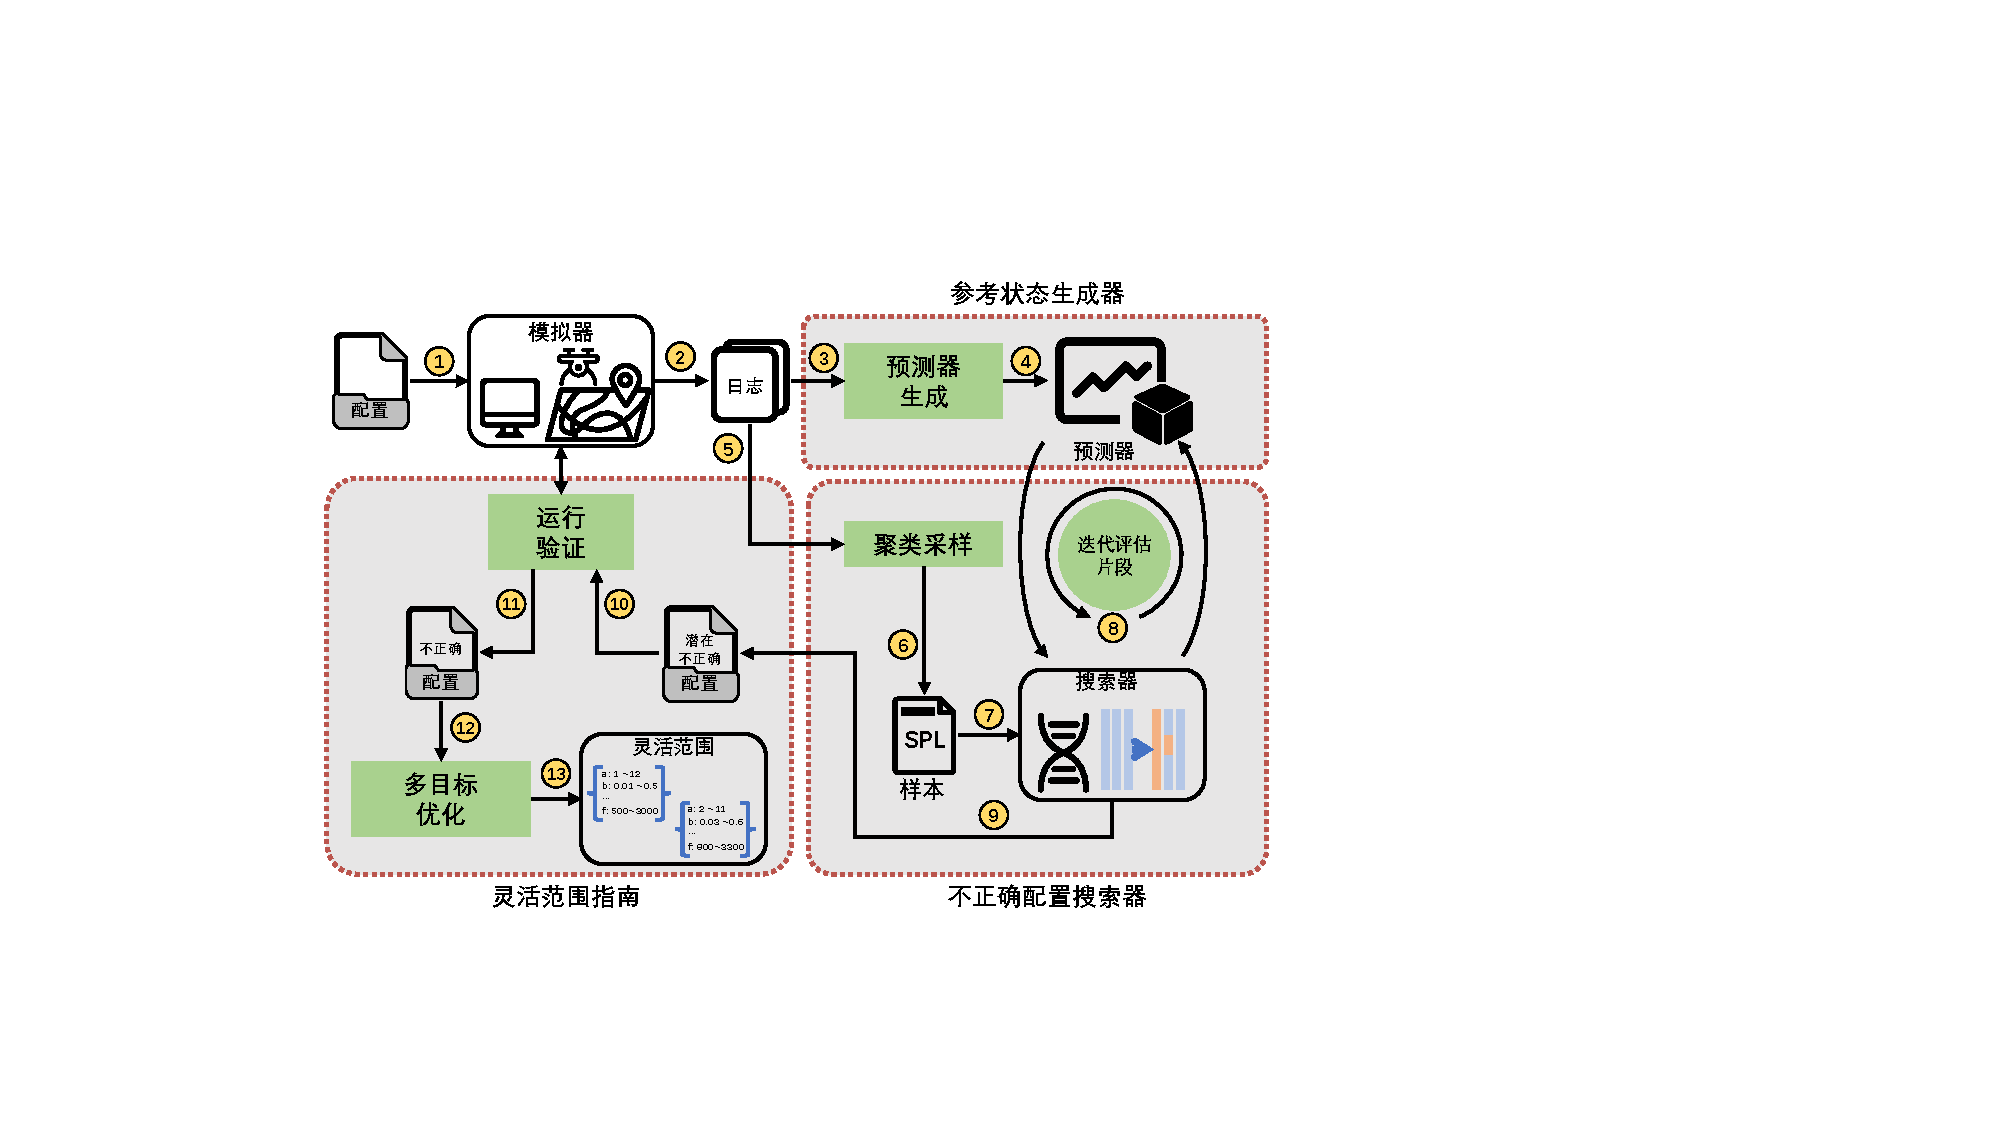
\includegraphics[width=\columnwidth]{fig/range/range_overview.pdf}
\caption{\icsearcher 流程概览.}
\label{fig:range_overview} 
\end{figure}

图~\ref{fig:range_overview}展示了\icsearcher 的整体框架所包含三个部分,包括\emph{参考状态生成器}、\emph{不正确配置搜索器}、和\emph{灵活范围指南},其各自功能的简单描述如下:

\begin{itemize}
\item \textbf{参考状态生成器:} 它采用历史飞行数据并创建一个预测器来预测飞行的状态变化,后续模块利用它来评估不正确的配置。
\item \textbf{不正确配置搜索器:} 它使用GA搜索模块来产生潜在的不正确配置。

\item \textbf{灵活范围指南:} 它应用多目标优化来提供安全的范围指南。

\end{itemize}

\icsearcher 的整体工作流程如下描述。
首先,由于预测器的生成和搜索器的搜索过程需要各种飞行数据。
\icsearcher 会利用一个模拟器并通过反复执行无人机飞行任务从而产生大量在不同的配置下的飞行数据(\circled{1}\circled{2})。
飞行日志数据被分成两部分,一部分被参考状态预测器采用用来生成预测器(\circled{3}),另一部分为搜索器提供关于飞行状态和传感器数据的基础数据(\circled{5})。
通过这些日志数据,系统训练一个能预测状态根据配置变化的预测器(\circled{4})。
对于不正确的配置搜索器,它对首先数据进行聚类,并从每个聚类组中抽取代表样本(\circled{6}\circled{7})。
然后搜索器会进一步针对这些样本进行启发式搜索,发掘潜在的不正确配置(\circled{8})。
比较特殊的是,在该搜索过程中,系统迭代地使用预测器来评估哪种配置有更高的概率导致不稳定状态。
搜索器的启发式搜索将在特定条件得到满足时停止。
当每个样本都通过搜索器获得了相应的潜在不正确配置后,他们会被构建成一个集合(\circled{9}),并通过模拟器飞行任务执行进行验证(\circled{10}\circled{11})。
最后,根据潜在不正确配置的验证结果,灵活的范围指南利用多目标优化来完善多个可用的可行范围指南,这些指南在某些特定条件下满足可用性和稳定性的最佳平衡(\circled{12}\circled{13})。

\subsection{飞行数据收集}\label{subsec:log_gen}
参考状态预测器是一个拥有未知参数的灰盒模型,需要大量数据进行拟合。
由于没有描述无人机输入/输出的标准数据集,为了构建一个预测器并为进一步搜索提供状态样本,该方案建立了一个飞行测试场景来收集飞行日志。
由于非默认配置的飞行可能导致不稳定的飞行,并进一步造成硬件损坏,对于飞行测试场景,该方案利用模拟飞行来收集飞行日志。
值得注意的是,考虑到强逆风或顺风等环境因素,即使使用默认配置,仍然可能发生崩溃。
这些飞行测试设定了不同的配置但设置了相同的飞行任务\tool{AVC2013}~\footnote{\url{https://avc.sparkfun.com/2013}},该任务通常用于测试无人机任务执行能力的,
对于用于训练预测器的数据,系统记录了飞行日志但舍弃了那些造成不稳定状态的,因为它们是不可控的和复杂的(与稳定状态数据相比)。
无人机中的不同数据模块有不同的类型的日志记录频率,本方案将其统一为10Hz,即0.1秒的间隔。
每个日志条目包含的状态信息包括角位置、角加速度、油门速度、GPS、陀螺仪和加速度计的传感器数据、当前设定的配置和时间戳索引。
对于该方案讨论的飞行控制程序,\tool{Ardupilot}和\tool{PX4},实验为 \tool{Ardupilot}记录了$740,799$的系统日志条目,为 \tool{PX4}记录了$410,962$的系统日志。
    
\subsection{参考状态预测器}
虽然利用GA模糊法可以减少参数的搜索空间,但参数组合(配置)的数量仍然很多,这使得通过现实/模拟执行进行验证的效率很低。
规避了采用飞行执行验证方式,本方案利用预测器来验证配置的影响对于无人机飞行的影响。
根据背景介绍中的说明,飞行控制算法根据之前的状态反馈、当前状态、传感器数据和加载的配置来估计下一个参考状态。
本方案应用机器学习(Machine Learning)预测器来模仿这个过程,学习他们的输入/输出相关性。
与原来的控制算法不同,由于预测器是用来拟合控制算法的,为了提高准确性,本方案的预测器考虑了多个历史反馈状态数据作为输入。
使用这种方法生成的预测器具有与控制算法相同的属性,可以估计参考状态,并且后续可以进一步评估配置如何影响飞行状态。
训练预测器的生成主要通过\emph{特征提取}和\emph{预测器生成}两个步骤所完成。


\subsubsection{特征提取}
无人机的日志条目中包含了许多无关信息,\icsearcher 通过选择特定的数据来构建特征向量。
因为并非条目中的所有项目在不稳定场景的影响下都具有可变偏差。
例如,即使无人机的姿态受到干扰,位置状态(高度、纬度、经度)也不会发生剧烈变化。
同样,温度传感器数据在整个任务过程中基本保持不变。
\param{BATT2\_VLT\_OFFSET}(电压偏移调整)和 \param{COMPASS\_OFS\_X}(X 轴上的罗盘偏移,单位为毫高斯)等参数不会影响姿态。
由于该方案的目标是分析影响飞行姿态(即角度和速度)的不稳定状态,因此在选取特征时主要考虑以下状态、传感器数据和配置。
(1) 飞行状态的角度位置和速度,表示为$a$。
(2) 从陀螺仪、加速度计和罗盘获得的传感器数据,表示为$e$。
(3) 调节姿态的控制或任务的参数集,表示为$c$。
根据上述信息,系统将它们分组为一个特征向量,$v\{a, e, c\}$,为了便于描述,定义$s=\{a,e\}$。
因此,在时间戳$t$时的数据所组成的特征向量应该为$v_t=\{s_t,c_t\}$。
这些向量被进一步组合以构建一个特征矩阵。

\subsubsection{预测器生成}
由于长短时记忆网络(LSTM)~\cite{hochreiter1997long}技术能有效地拟合复杂的输入/输出关系~\cite{stock,highway,selvin2017stock},\icsearcher 使用\tool{LSTM}作为预测器来预测下一个参考状态。
预测器将时间戳小于等于$t$的若干$h$连续向量作为输入(即$V\{v_{t-h-1},...,v_{t-1},v_{t}\}$),从而预测输出下一个预测的向量$v'_{t+1}$中的参考状态$a'_{t+1}$,后续的实验将会确定使用多少个历史向量$h$较为合适。
在训练阶段,LSTM采用\tool{平均平方误差 (Mean Squared Error,MSE)}~\cite{4775883}来迭代优化预测器的内部权重,确保预测的状态$a_{t+1}'$足够接近于地面真实状态$a_{t+1}$。

虽然预测器是指定给某个控制程序的,但预测方案是可以根据相应的控制程序(即动态模型、控制算法、配置参数和数据采样方法)来扩展的。
也就是说,虽然为某一控制程序生成的预测器不能直接用于其他控制程序,但是生成预测器的模板是通用的,不同的飞行控制程序可以提取相同的格式状态和传感器数据来实例化预测器以估计参考状态。

\subsection{不正确配置搜索器}
为了搜索引发不稳定偏差(即参考状态和当前状态之间存在严重偏差)的不正确配置,本搜索方案以历史飞行数据中存在的飞行状态为基础,开展模糊搜索测试以找出具有高概率导致这个基础状态出现较高偏差的潜在配置。
方案从历史的飞行数据中聚类出具有代表性的状态片段样本,然后从用遗传算法(GA),一种元启发式搜索的方法搜索在该状态样本的背景下,什么样的配置会引发参考状态和实际状态出现偏差变大的情况(即产生不稳定), 并将这些配置称之为\emph{潜在不正确配置}。

具体而言,对于排除了配置元素的$N$个原始飞行条目$Raw=\{v_{1},v_{2},...v_{N}\}$,搜索器首先将其分成多个段$S_{t}, t \in [1,N]$ 作为候选片段。
具体的每个段得生成方式如下。
\begin{equation}
    S_{t}=\{v_{t},v_{t+1},...,v_{t+len-1}\}, t~mod~(t+len) = 0
\end{equation}
其中$t$是记录数据的索引,$len$是每个片段的长度。
飞行过程中的噪声或者瞬时误差都会对预测器产生影响,因此,为了排除瞬时误差对整个搜索的影响,搜索器将每个段的长度设定为$10+h$(即$len=10+h$)。
同时由于重复配置的相似段数据可能会降低搜索效率,因此,系统采用先聚类后抽样的方法选择有代表性的样本进行搜索,这样可以在保持多样性的同时减少冗余。
\icsearcher 首先使用\tool{DBSCAN}~\cite{schubert2017dbscan},一种基于概率密度的非参数自适应聚类算法,对这些样本数据片段进行聚类,并从每个聚类组中随机抽取$m_{2}$个代表数据样本。
对于每一个数据片段,GA搜索器启动,依靠突变、交叉和选择这些遗传算法的迭代流程来进行搜素相应的不正确配置。
最后,所有样本片段的搜索结果都被合并且去掉重复,成为一个独特的集合,被称为\emph{潜在不正确配置集合}。
接下来的内容将详细介绍关键的步骤,即关于如何评估配置的 \emph{预测器片段评估}和关于搜索器如何工作的\emph{搜索过程}。

\subsubsection{预测器片段评估}
通过使用预测器,GA搜索应用适应度来量化一个配置在特定环境(状态和传感器数据)下可能造成的偏差程度。
预测器对于片段数据的评估创建了一个得分来描述该配置可能造成的偏差的。
分数越高,说明预测器认为这种配置越是\dquote{危险},否则就越是\dquote{安全}。

假设当前的模糊搜索是针对上下文片段$S\{v_{1},v_{2},...,v_{10+h}\}$进行的。
给定一个待评估的配置$c\{p_1,p_2,...,p_{n2}\}$($n2$是参数的数量)时。
片段评估函数将其与段合并以创建特征向量$V\{\{v_1, c\}, \{v_2, c\},...,\{v_{10+h}, c\}\}$。
然后,该函数用一个滑动窗口将$V$分成长度为$h+1$的块。
\begin{equation}
    B = \{b_{1}, b_{2}, ..., b_{10}\} 
\end{equation}  
其中每个块$b_{t}$ 是:
\begin{equation}
    b_{t} = \{v_{t}, v_{t+1}, ..., v_{t+h}\}, t\in[1, 10] 
\end{equation}
对于每个块$b_{t}$,$b_{in}=\{v_t,v_{t+1},...,v_{t+h-1}\}$被用作输入,$v_{t+h}$中的$a_{t+h}$被用作真实状态数据。
也就是说$b_{in}$被作为预测器的输入用来估计参考状态$a'(t+h)$。
一个单一的偏差是预测状态和真实状态之间的一范数,也就是$d = \Vert a_{t+h} - a'_{t+h} \Vert$。  
而一个片段包含有$10$个块,也就可以划分$10$组输入和真实输出。
进一步的也就能够计算出10个偏差$D=\{d_1, d_2, ..., d_{10}\}$,对应到原始数据当中,也就是$1$秒内的偏差。
这个配置$c$的适应度评价是这些偏差的总和$D_{sum}=\sum_{i=1}^{10}{d_i}$。
搜索的目标是找出那些被预测为适配度最大化的配置,也就是有较大概率引起不稳定状态的个体(此处指配置)。


\subsubsection{搜索流程}
对于一个片段数据$S$,搜索器分配具有默认参数值的种群(配置组),种群中的每一个个体表示一个配置。
假设种群大小为$NP$,最大迭代次数为$G_{max}$。
搜索过程中对该种群进行反复变异和更新,具体过程如下。

假设当前迭代代数为第$g$代($g\in[1,G_{max}]$),搜索器首先对当前种群
\begin{equation}
pop_g=\{c_{1,g},c_{2,g}...,c_{NP,g}\}   
\end{equation}
进行变异,生成变异种群
\begin{equation}
pop_v=\{y_{1,g},y_{2,g},...,y_{NP,g}\}
\end{equation}
变异种群的每个配置都是按以下方式计算。
\begin{equation}
    y_{i,g} = c_{i,g} + F * (c_{best,g} - c_{i,g}) + F * (c_{r1,g} - c_{r2,g})
\end{equation}
其中$c_{r1/r2,g}$为种群中的一个随机个体(配置)。
$c_{best,g}$是那一代中最佳适应度的个体,而$F$为比例因子。

然后搜索器对$pop_g$和$pop_v$进行交叉运算,产生一个新的实验种群:
\begin{equation}
    pop_e=\{ec_{1,g},...,ec_{NP,g}\}
\end{equation}
其中
\begin{equation}
    ec_{i,g}=\{ec_{i1,g},ec_{i2,g},...,ec_{ij,g}\},i \in [1,NP], j \in[1,D]
\end{equation}
一个配置中的参数值$ec_{ij,g}$可按如下方式获得:
\begin{equation}
    ec_{ij,g}=\begin{cases}
y_{ij,g}, & if~rand(0,1) < CR~or~j=j_{rand}\\
c_{ij,g}, & otherwise
\end{cases}
\end{equation}  
其中$j_{rand}$是$[1,D]$中的一个随机整数、
$CR$是交叉率、
$c_{ij,g}$是$pop_g$中第$i$配置的第$j$个参数值、
和$y_{ij,g}$是$pop_v$中第$i$种配置的第$j$个参数值。

搜索器使用\emph{预测器片段评估}中的方法来计算$pop_g$和$pop_e$中个体的分数。
根据它们的得分,搜索者从群体中选择配置,用以下方法创建下一代$pop_{g+1}$:
 \begin{equation}
    c_{i,g+1}=\begin{cases} 
ec_{i,g}, & if~f(ec_{i,g})<f(c_{i,g})\\
c_{i,g}, & otherwise
\end{cases}
\end{equation}   
其中$f$是\emph{预测器片段评估}。

最终,如果种群的适应性不再增加,或者迭代达到最大数量$G_{max}$。
搜索器就会停止,最后一代种群中得分最高的前$10$的个体被认为是潜在的不正确配置。
    
\subsection{灵活范围指南}
根据搜素器提供的潜在不正确配置,\icsearcher 需要总结出一个新的范围指南。
使用者在参考这个范围指南后会减少出现不正确配置的可能性,从而进一步减少触发不稳定飞行状态的可能性。

\subsubsection{执行验证} 
搜索结果是潜在不正确的配置,意味着这些配置有很高的概率导致不稳定的状态,但是它们是否是不正确的仍然需要通过飞行执行测试来验证。
因此,\icsearcher 利用飞行模拟器平台来测试这些配置对无人机飞行带来的影响,观察哪些配置会导致真正的不稳定状态。
与收集阶段类似,无人机用这些配置设置来执行\tool{AVC2013}任务。

\subsubsection{范围指南生成} 
参数范围指南的目标是防止用户上传不稳定的配置。
但是上述搜索器所发现的不正确配置是离散地存在于可配置空间中的,而范围指南只能是连续的可配置空间,因此就面临一个问题。
给出较小的可配置空间确实能够极大地避免不正确配置地空间,有效地确保了稳定性。
但是相应地,其可配置的范围变小,这并不利于用户的实际使用需求,也就是降低了适应性。
因此,\icsearcher 不提供一个具体的范围指南,而是利用多元优化来确定灵活的范围指南。
\icsearcher 主要基于以下考虑提供灵活的范围指南。
(1)随着参数数量的增加,很难完全排除不安全的参数值,因为安全参数范围可能不连续。
(2)虽然稳定性是最重要的,用户可能愿意为更好的控制灵活性或可用性承担一些小的风险。
如果一个配置中的所有参数值都在指南规定的范围内,则认为该配置已被覆盖。
\icsearcher 将范围指南($Range'$)的生成视为以下优化问题。

\begin{equation}
\begin{cases}
        min~f_1 = \frac{num(R_{incorrect } \in Range')}{num(R \in Range')}   \\
       max~f_2 = num(R \in Range')  \\
       s.t. &\\
       Range' \in OriginRange
\end{cases}
\label{eq1}
\end{equation} 

优化问题涉及两个目标:
(1) 尽可能利用验证结果,使指南所涵盖的验证配置$R$的数量最大化。
(2)尽可能保持安全,以最小化不正确配置的覆盖范围$R_{incorrect}$。
实际上,缩小不正确配置的覆盖范围也会缩小每个参数值的范围,反之亦然。
因此,与其为每个参数定义严格的范围。
系统用多个约束条件来解决这个优化问题,以构建一个多样化的\tool{Pareto}边界解决方案组。
这些\tool{Pareto}解决方案形成了一个由最佳可行方案组成的边界。
允许用户可以从边界位置选择最符合他们需的方案来平衡他们任务的要求中的安全性和适应性。 



\section{实验结果及分析}
本章节通过考虑其在验证配置方面的有效性和效率来评估\icsearcher 。
\begin{itemize}
 
\item \textbf{研究问题1 有效性:} \icsearcher 能精确检测出来少不正确的配置?

\item \textbf{研究问题2 适应性:} \icsearcher 可以为参数提供最合适的值范围?

\item \textbf{研究问题3 提升:} 突变和预测器是如何帮助改善配置验证的?

\end{itemize}

\subsection{实验设定}

\begin{itemize}
    \item \textbf{实验程序:}
本章节将 \icsearcher 应用于两个流行的开源飞行控制程序。
\tool{ArduPilot} (4.2.0)~\cite{ardupilot} 和 \tool{PX4} (1.13)~\cite{px4}, 这些工具被无人机制造商广泛使用,如\tool{Parrot}、\tool{Mamba}和\tool{Mateksys}~\footnote{\url{https://ardupilot.org/copter/docs/common-autopilots.html\#closed-hardware}}。

\item \textbf{测试设备:}
为了验证\tool{ArduPilot}和\tool{PX4}中规定的配置,本此实验利用四个实验飞行器(如图~\ref{fig:range_pix}所示)进行测试,其中包括两个装有\tool{Pixhawk}的无人机~\cite{meier2011pixhawk}。(\tool{CUAV ZD550}和\tool{AMOVLab Z410}),两个无人机模拟器(\tool{Airsim}~\cite{airsim2017fsr},\tool{Jmavsim}~\footnote{\url{https://dev.px4.io/v1.10_noredirect/en/simulation/jmavsim.html}})。

\begin{figure}[htb]
\centering{
\subfloat[CUAV ZD550]{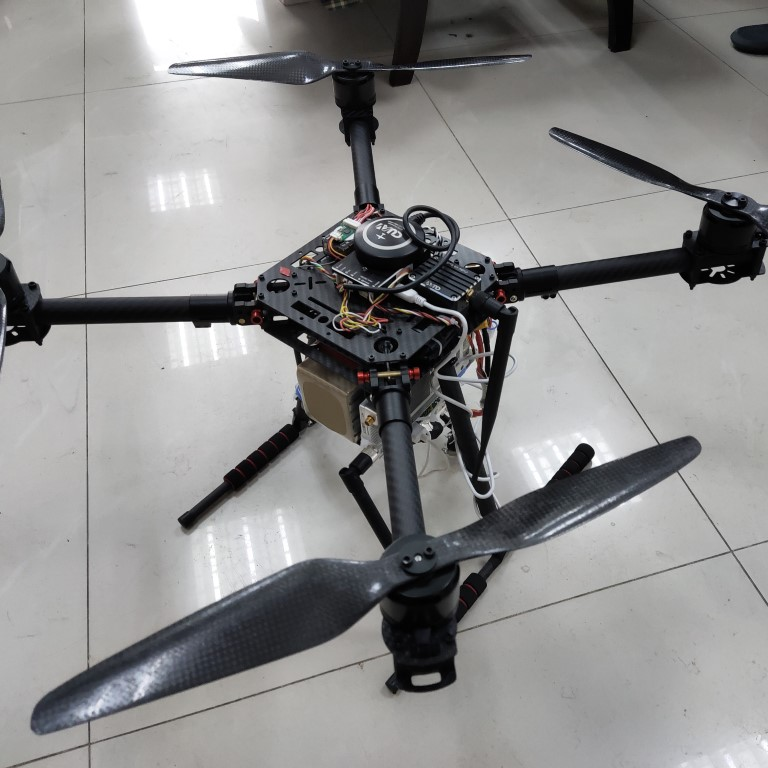
\includegraphics[width=0.3\linewidth]{fig/range/real/px1.jpg}}\quad
\subfloat[AMOVLab Z410]{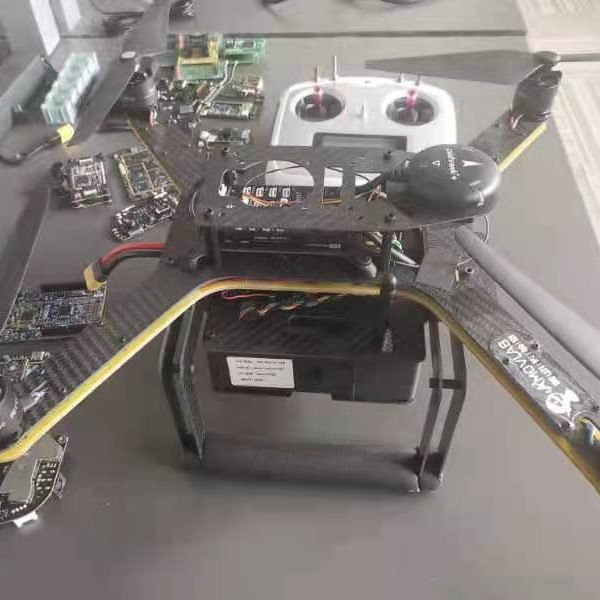
\includegraphics[width=0.3\linewidth]{fig/range/real/px2.jpg}}
}

\centering{
\subfloat[Airsim]{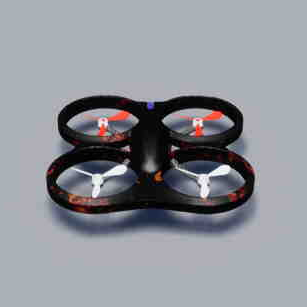
\includegraphics[width=0.3\linewidth]{fig/range/real/airsim.png}}\quad
\subfloat[Jmavsim]{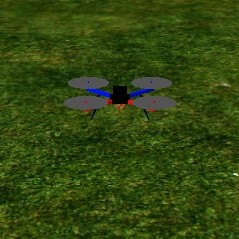
\includegraphics[width=0.3\linewidth]{fig/range/real/jmavsim.jpg}}}
\caption{用于实验的真实和虚拟无人机车辆}
\label{fig:range_pix}
\end{figure}

\item \textbf{参数选择:}
根据制造商提供的控制参数描述。
后续实验为\tool{Ardupilot}选择了20个参数(表~\ref{tab:range_paramall}),为\tool{PX4}选择了14个参数(表~\ref{tab:range_paramall_px4}),可能影响飞行角位置和角速度。
需要说明的是,一个预测器对特定的飞行控制程序是有效的,所以对于\tool{Ardupilot}和\tool{PX4}使用相同的架构结合各自的数据分别产生预测器。


\begin{table*}[htb]
\centering
\begin{minipage}{0.49\linewidth}
\small
\caption{用于实验的Ardupilot控制程序的参数}
\label{tab:range_paramall}
\centering
\begin{tabular}{ccc}
        \toprule[1.5pt]
         参数 & 官方范围 & 默认值 \\
        \midrule[0.8pt]
         PSC\_VELXY\_P & [0.10, 6.00] & 2.0 \\ 
       
         PSC\_VELXY\_I & [0.02, 1.00] & 1.0 \\
       
         PSC\_VELXY\_D & [0.00, 1.00] & 0.5 \\
       
         PSC\_ACCZ\_P & [0.20, 1.50] & 0.5 \\
       
         PSC\_ACCZ\_I & [0.00, 3.00] & 1.0 \\
       
         ATC\_ANG\_RLL\_P & [3.00, 12.0] & 4.5 \\
       
         ATC\_RAT\_RLL\_P &  [0.01, 0.50] & 0.135 \\
        
         ATC\_RAT\_PIT\_I & [0.01, 2.00] & 0.135 \\
        
         ATC\_RAT\_RLL\_D & [0.00, 0.05] & 0.0036 \\
        
         ATC\_ANG\_PIT\_P & [0.00, 12.0] & 4.5 \\
       
         ATC\_RAT\_PIT\_P & [0.01, 0.50] & 0.135 \\
        
         ATC\_RAT\_PIT\_I & [0.01, 2.0] & 0.135 \\
        
         ATC\_RAT\_PIT\_D & [0.00, 0.05] & 0.0036 \\
       
         ATC\_ANG\_YAW\_P & [3.00, 12.0] &4.5 \\
       
         ATC\_RAT\_YAW\_P & [0.10, 2.50] & 0.18 \\
       
         ATC\_RAT\_YAW\_I & [0.01, 1.00]& 0.018 \\
       
         ATC\_RAT\_YAW\_D & [0.00, 0.02] & 0 \\
         
         WPNAV\_SPEED & [20, 2000] & 500 \\
       
          WPNAV\_ACCEL & [50, 500]& 100 \\
       
       ANGLE\_MAX & [1000, 8000] & 4500 \\
        \bottomrule[1.5pt]
\end{tabular}
\end{minipage}
\begin{minipage}{0.49\linewidth}
\small
\caption{用于实验的PX4控制程序的参数}
\label{tab:range_paramall_px4}
\centering
\begin{tabular}{ccc}
        \toprule[1.5pt]
          参数 & 官方范围 & Default \\
        \midrule[0.8pt]
         MC\_ROLL\_P & [0.00, 12.0] & 6.5 \\
       
         MC\_PITCH\_P & [0.00, 12.0] & 6.5 \\ 
       
         MC\_YAW\_P & [0.00, 5.0] & 2.8 \\ 
        
         MC\_YAW\_WEIGHT & [0.00, 1.00] & 0.4 \\ 
        
         MPC\_XY\_P & [0.00, 2.00] & 0.9 \\ 
        
         MPC\_Z\_P & [0.00, 1.50] & 1.0 \\ 
        
         MC\_PITCHRATE\_P & [0.01 0.60] & 0.15 \\ 
        
         MC\_ROLLRATE\_P & [0.01, 0.50] & 0.15  \\ 
        
         MC\_YAWRATE\_P & [0.00, 0.60] & 0.2 \\ 
        
         MPC\_TILTMAX\_AIR & [20.0, 89.0] & 45.0 \\ 
        
         MIS\_YAW\_ERR & [0.00, 90.0] & 12.0 \\
        
         MPC\_Z\_VEL\_MAX\_DN & [0.5, 4.0] & 1.0 \\
        
         MPC\_Z\_VEL\_MAX\_UP & [0.5, 8.0] & 3.0 \\
        
         MPC\_TKO\_SPEED & [1.0, 5.0] & 1.5  \\
        
        \bottomrule[1.5pt]
\end{tabular}
\end{minipage}
\end{table*}

\item \textbf{模型和搜素设定:}
预测器和GA搜索器是用Python实现的。
对于GA,其进化停滞判断阈值被设定为$0.1$、代表数$m_{2}$被设定为$10$、最大的进化代数被设定为$200$、
初始种群的大小为$500$(即$NP=500$)、比例因子$F$为0.4。

\end{itemize}


\subsection{研究问题1: 有效性}
实验首先对\icsearcher 在\tool{Ardupilot}和\tool{PX4}两个不同飞控情况下进行评估,计算了飞行状态预测阶段预测器的预测精度。
然后实验验证了预测的不正确配置是否会影响飞行稳定性。

\subsubsection{状态预测}
首先利用章节~\ref{subsec:log_gen} 中的日志数据为 \tool{Ardupilot} 和 \tool{PX4} 创建预测器,其中 90\% 的数据用于训练,10\% 用于测试。
最后根据实验结果确定最佳输入长度$h$。
预测器的预测精准度结果如表~\ref{tab:range_acc}所示。
从表中可以观察到,不同长度的输入会对预测的准确性产生轻微的影响。
为了后续实验的准确性,根据这些结果,后续实验选择精度最好的预测器,即输入长度h=4来进行相关的测试。

\begin{table}[ht]
\caption{不同输入长度的测试数据的预测精度}
\label{tab:range_acc}
\centering
\begin{threeparttable}
\begin{tabular}{c|ccccc}
        \toprule[1.5pt]
        $h$  & 2 & 3 & 4 & 5 & 6 \\
        \midrule
        

        Ardupilot  & 96.05\% & 96.19\% & 97.10\% & 95.60\% & 95.77\% \\

        PX4 & 94.32\% & 95.56\% & 96.15\%  & 94.52\% & 94.45\% \\

        \bottomrule[1.5pt]
\end{tabular}
% \begin{tablenotes}
% \footnotesize
% \item[*] Ardu is Ardupilot.
% \end{tablenotes}
\end{threeparttable}
\end{table}

此外,实验选择了两个个飞行日志(\tool{Ardupilot}和\tool{PX4})中的数据用来展示了预测和实际状态变化之间的差异。
通过将日志中的数据进行相同的预处理操作并输入到训练好的预测其中输出预测结果。
图~\ref{subfig:range_diff1} 和图~\ref{subfig:range_diff2} 中展示了预测器输出的预测状态和实际状态的的对比图。
图中虚线曲线表示实际状态,实线表示预测状态,底部的直方图(青色条)表示两条曲线之间的差异。
该图表明预测器准确地预测了状态变化的趋势,与实际值非常匹配。



\begin{figure*}[htb]
\centering
\begin{minipage}{0.49\linewidth}
    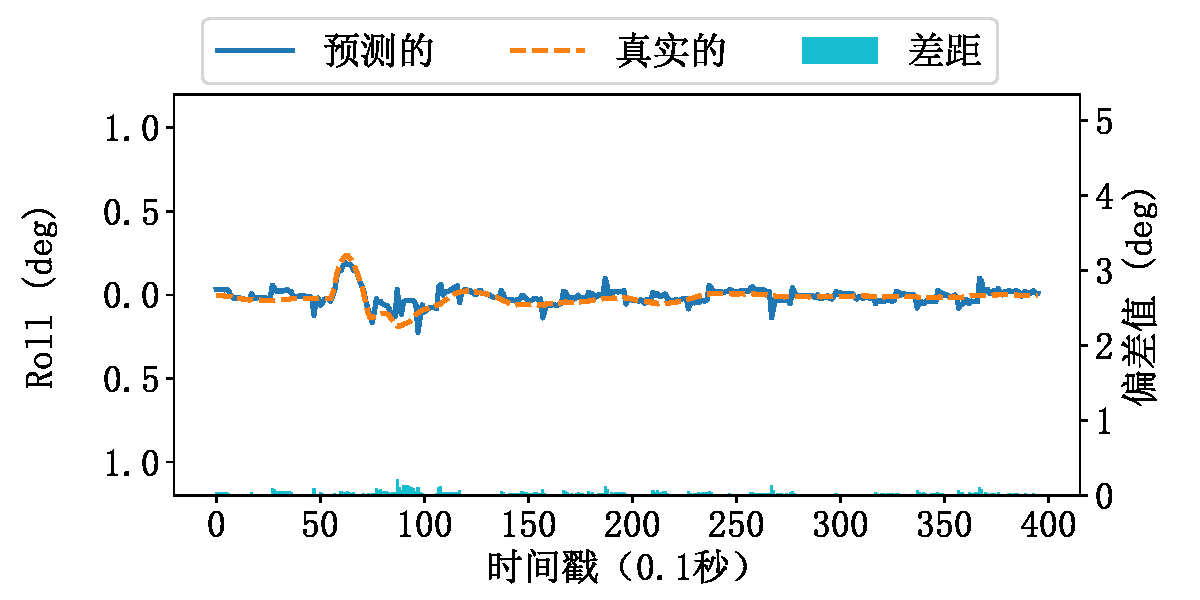
\includegraphics[width=\linewidth]{fig/range/ardu_real_roll.pdf}\quad
    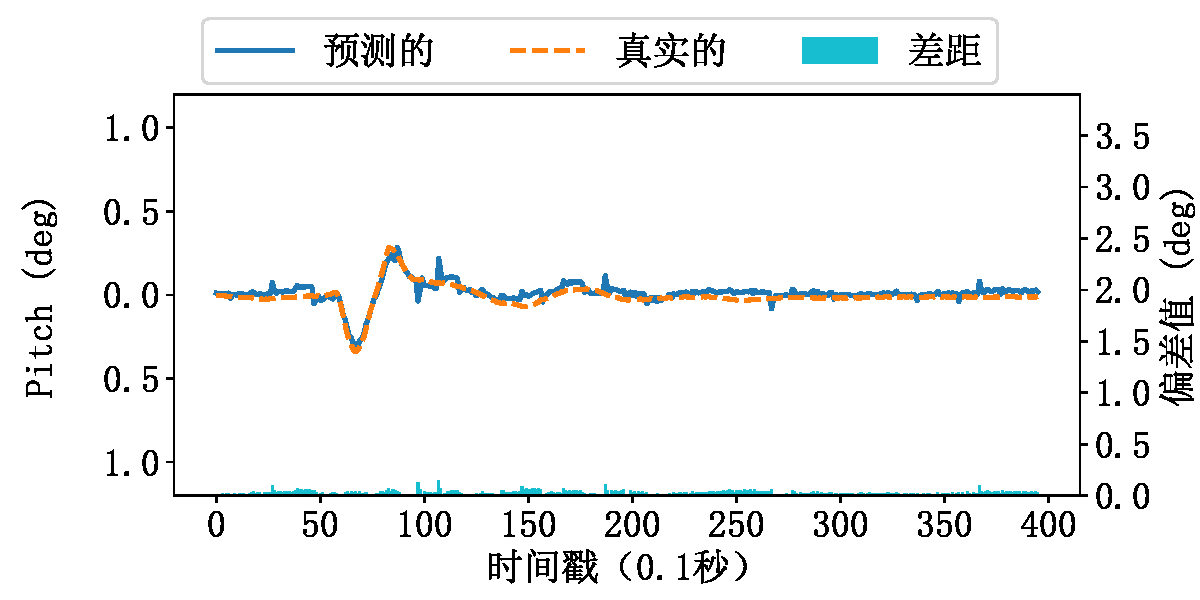
\includegraphics[width=\linewidth]{fig/range/ardu_real_pitch.pdf}\quad
    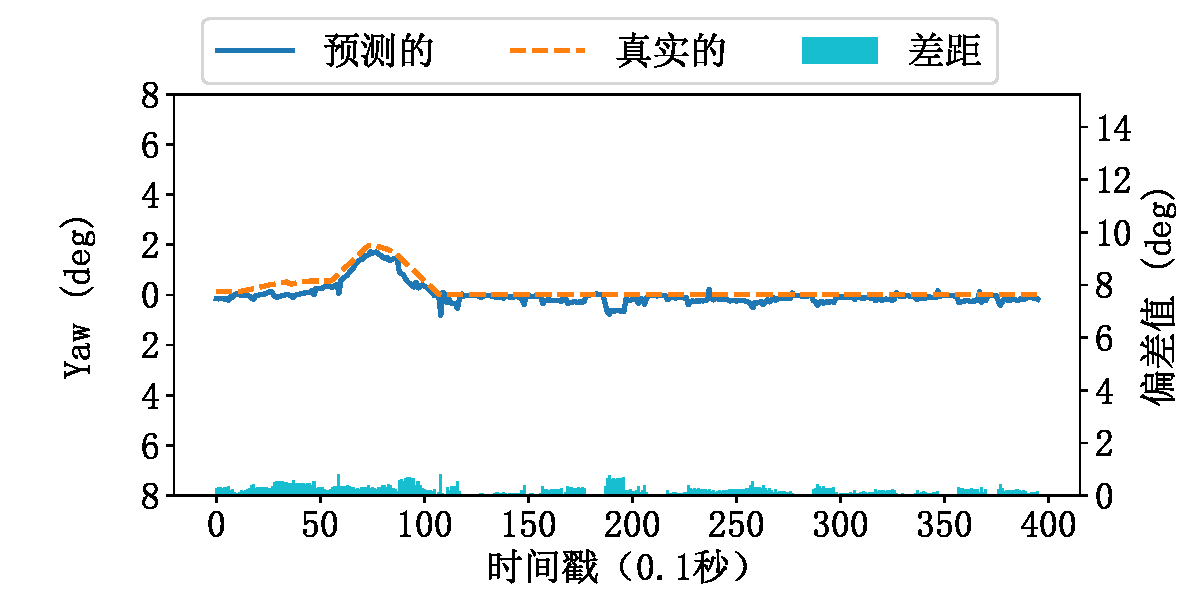
\includegraphics[width=\linewidth]{fig/range/ardu_real_yaw.pdf}
    \caption{Ardupilot 状态变化(Roll, Pitch, 和 Yaw)}
    \label{subfig:range_diff1}
\end{minipage}
\begin{minipage}{0.49\linewidth}
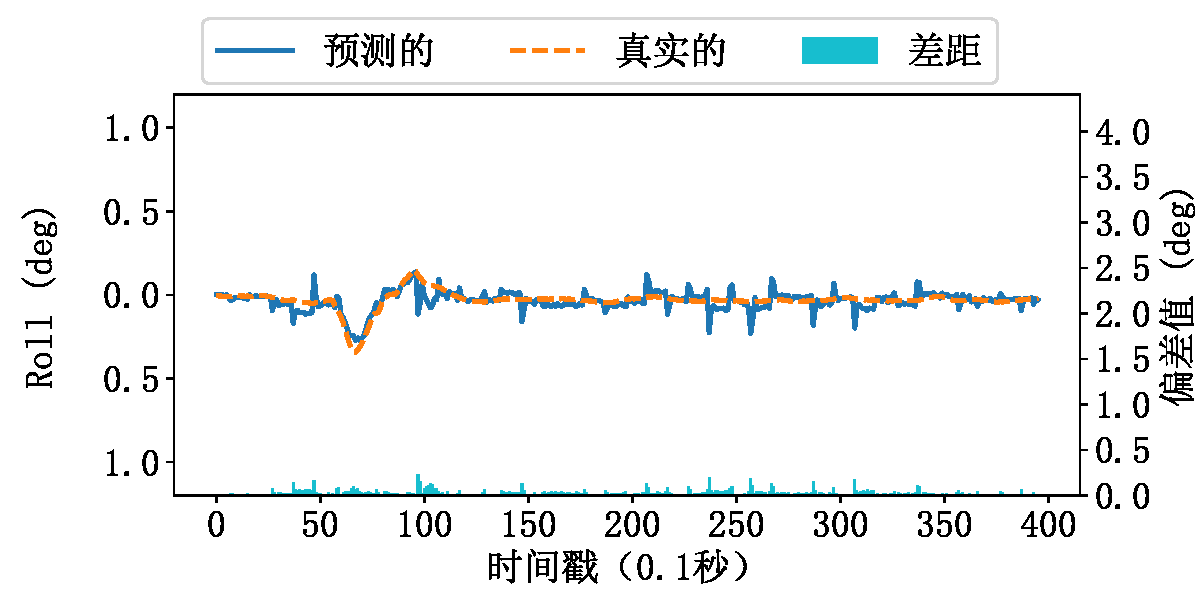
\includegraphics[width=\linewidth]{fig/range/px4_real_roll.pdf}\quad
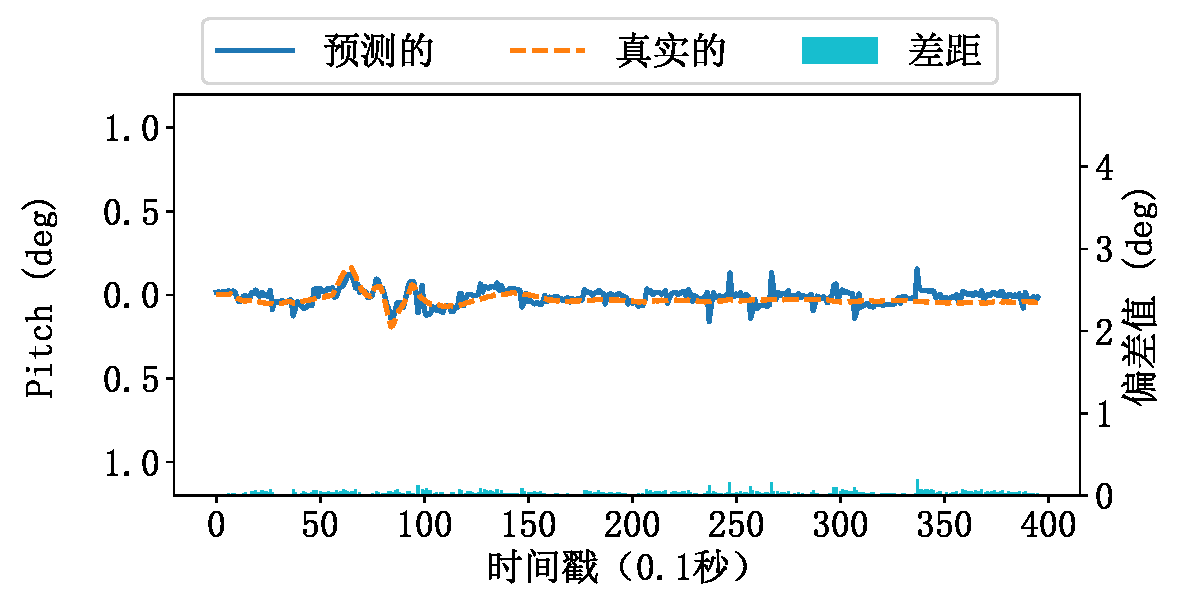
\includegraphics[width=\linewidth]{fig/range/px4_real_pitch.pdf}\quad
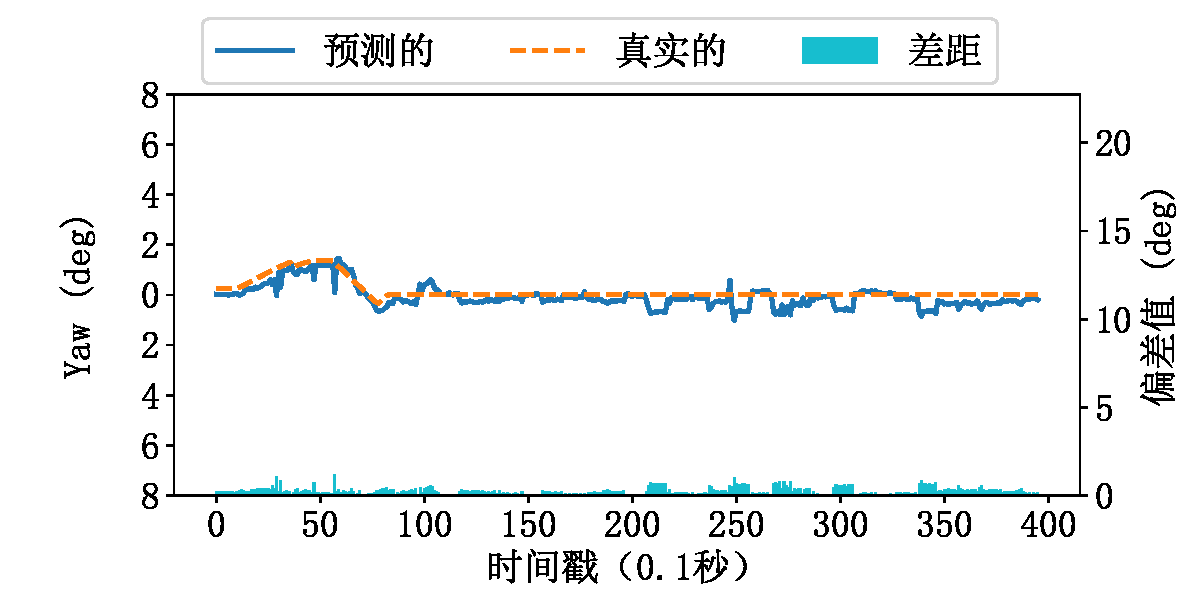
\includegraphics[width=\linewidth]{fig/range/px4_real_yaw.pdf}
\caption{PX4状态变化(Roll, Pitch, 和 Yaw)}
\label{subfig:range_diff2}
\end{minipage}
\end{figure*}

正如前文所述,一个合格的预测器应该能够辅助\icsearcher 准确的区分稳定状态和不稳定状态。
\icsearcher 可以利于预测器来识别更有可能触发不稳定状态的配置从而进模糊测试的迭代过程。
为了证明所生成的预测器的有效性,实验以\tool{Ardupilot}为例,进行了简单阈值分类测试,同时与之前的较为优秀的方法所提出的\tool{LGDFuzzer} 中的预测器进行性能比较。
\tool{LGDFuzzer} 中的预测器是根据预测值和实际值之间的单个偏差来预估配置导致不稳定状态的可能性。
作为对比,本方案中的\icsearcher 则是计算段偏差(段内偏差之和)来做出此确定。

具体来说,此对比实验进行了2,000次飞行测试,其中1,542个由于严重事件而未能完成任务,而458个成功完成任务。
该实验使用2,000个配置中的1,600个(考虑了其中的类别权重)来计算阈值,其余 400 种配置用于测试目的。
当分析包含严重事件(标记为不稳定)的测试日志时,\icsearcher 会提取严重事件时间戳之前发生的片段数据的偏差。
相反,\tool{LGDFuzzer} 仅考虑严重事件时间戳之前发生的单个数据的偏差。
对于不包含严重事件的稳定测试日志(标记为稳定),\icsearcher 随机记录一个段的数据并求其偏差,而 \tool{LGDFuzzer} 随机选择的依旧是单个偏差值。
为了确定阈值,实验计算了稳定 ($ST_{avg}$) 和不稳定 ($UST_{avg}$) 数据的平均分段/单个偏差,然后将阈值设置为这两个平均值之间的中点,即 $(ST_{avg} + UST_{avg}) / 2$。


表~\ref{tab:cross} 显示了通过1600个数据计算出的阈值以及400个测试数据中不稳定的检测性能。
其中片段偏差方案为\icsearcher ,单一偏差方案为 \tool{LGDFuzzer}。
根据表中各自的平均偏差值,片段方案的阈值是3.25,而单一方案的阈值为0.24。
在测试数据中,如果数据超过上述规定的阈值,则被标记为不稳定。

片段偏差方案和单一偏差方案都表明,不稳定状态比稳定状态表现出更大的偏差。
预测器在GA过程中可以利用这一特性来提升模糊测试的效率。
预测器可用通过预测偏差来将配置驱动到更高的偏差值从而诱发不稳定飞行的配置。
与之前未能获得超过 90\% 的 F1-Score的 \tool{LGDFuzzer} 方法相比,\icsearcher 在 F1-Score方面表现更好。
这种改进可归根于片段偏差的使用, 它通过聚合片段内的所有偏差来进行判断,从而减轻了预测器自身准确性的影响,保证了较小的数值波动。
换句话说,在模糊测试中使用片段偏差方法可以更准确地预测某个配置是否会导致不稳定状态。

\begin{table}[ht]
\caption{稳定/不稳定的平均偏差和分类性能}
\label{tab:cross}
\centering
\begin{threeparttable}
\begin{tabular}{c|ccc|ccc}
        \toprule[1.5pt]
        & \makecell*[c]{稳定数据} & \makecell*[c]{不稳定数据}  & 阈值 &
        Precision & Recall & F1-Score \\
        \midrule[0.8pt]

        片段偏差方案 & 1.72 & 4.77 & 3.25 & 92.48\% & 98.19\% & 95.25\% \\

        单一偏差方案 & 0.15 & 0.34 & 0.24 & 80.99\% & 98.19\% & 89.01\% \\
        \bottomrule[1.5pt]
\end{tabular}
\end{threeparttable}
\end{table}

\subsubsection{配置验证}
实验应用测试数据,也就是~\ref{subsec:log_gen} 节中指定的剩余10\%日志数据来进行配置验证实验。
该数据集包括74,074个\tool{Ardupilot}日志条目(总计5,698个片段)和41,096个\tool{PX4}日志条目(总计3,161个片段)。
根据\icsearcher 中的步骤,这些数据被划分为为58和33个簇。
\icsearcher 从每个簇中提取10个样本(如果少于 10 个则为所有可用样本)。
实验总共包含571个片段样本用于测试\tool{Ardupilot},316个片段样本用于测试\tool{PX4}。

随后,实验针对这些样本片段进行模糊搜索,以发掘潜在的错误配置。
对于发现的错误配置,实验再次启动的飞行验证,通过将这些配置上传到无人机并进行飞行以验证是否真的会造成问题。
对于\tool{Ardupilot},\icsearcher 发现了$4,386$个的不重复的潜在不正确配置。
经过模拟器的执行验证,在$4,386$的配置中,有$4,157$被标记为真正不正确的配置,其中分别包括$2,15$个\emph{轨迹偏航}、
$432$\emph{飞行冻结}、
$9$\emph{飞行坠毁}、
$2$\emph{启动后的特权升级}、
和$1,564$\emph{潜在动力损失}。
同样地,对于\tool{PX4},系统发现了$2,282$的潜在不正确配置。
经过验证,$2282$个潜在不正确配置中的$2087$被验证为真正的不正确配置,分别包括$641$\emph{轨迹偏航}、
$228$\emph{飞行冻结}、
$309$\emph{飞行坠毁}、 以及
$909$\emph{启动后的特权升级}。

由于飞控程序设计的原因,两个飞控本身存在差异,例如从传感器驱动程序获取的原始数据、参数列表、飞控算法和日志结构,因此实验结果存在差异。
结果表明,\tool{Ardupilot} 更容易导致轨迹偏差和潜在的推力损失,而 \tool{PX4} 则表现出更高的启动后特权升级和崩溃率。
这是因为\tool{PX4}额外采用了一个模型来检查当前配置是否会导致理论上的最大速度超过阈值,从而决定无人机是否应该起飞。
但是,如果在飞行期间发送这些被曾被拒绝的配置,飞控程序仍然会接收这些配置。
因此,相比\tool{Ardupilot},它导致了更多的启动后权限升级。

\subsection{研究问题2: 适应性}
为了证明系统的灵活范围指南的适应性,本实验利用上一章节已经确认的不正确配置($4,157$个)的结果来生成范围指南。
参照验证结果,灵活的范围指南为\tool{Ardupilot}提供了$178$个\tool{Pareto}解决方案,为\tool{PX4}提供了$213$个\tool{Pareto}解决方案。
每个\tool{Pareto}解决方案代表一个建议的配置范围。
如果范围包含不正确的比例小,可用的数值空间也越小,相应的,也就越安全。
范围包含不正确的比例越大,则可用的数值空间也越大,但是对应的页越危险。

\begin{table}[ht]
\caption{Ardupilot可行范围指南的例子}
\label{tab:range_shrink_cmp}
\centering
\begin{threeparttable}
\begin{tabular}{c|ccc|ccc|ccc}
        \toprule[1.5pt]
          \multirow{2}{*}{参数}  & \multicolumn{3}{c|}{\textit{指南1}} & \multicolumn{3}{c|}{\textit{指南2}} & \multicolumn{3}{c}{\textit{指南3}} \\
         \cmidrule[0.8pt]{2-10}
          ~ & {下界} & 上界 & 减少& {下界} & {上界} & 减少& {下界} & {上界} & 减少 \\
         
         \midrule[0.8pt]
        
        
          PSC\_VELXY\_P  &  0.3 &  5.9   & -5.1\%&  0.3 & 6.0  & -3.3\%  & 0.3 & 6.0   & -3.3\%\\
        
          PSC\_ACCZ\_I  &  0.0 &  2.9   & -3.3\%&  0.0 & 2.4  & -20\%  & 0.0 & 2.6  & -13.3\%\\
        
          ATC\_RAT\_RLL\_P &   0.13 &  0.37   & -51.0\%&  0.125 & 0.375  & -48.9\%  & 0.12 & 0.38  & -46.9\%\\
        
          ATC\_RAT\_RLL\_I &   0.01 &  0.46   & -77.3\%&  0.015 & 0.445  & -78.3.\%  & 0.01 & 0.915  & -54.5\%\\
        
          ATC\_RAT\_PIT\_P &   0.05 &  0.50   & -8.1\%&  0.05 & 0.50  & -8.1\%  & 0.055 & 0.475  & -14.2\%\\
    
          ATC\_ANG\_YAW\_P &   3.1 &  11.9   & -2.2\%&  3.1 & 12.0  & -1.1\%  & 3.0 & 12.0 & -0.0\%\\
        
          WPNAV\_SPEED &   750 &  2000   & -35.8\%&  700 & 2000  & -33.3\%  & 800 & 2000  & -38.4\%\\
         
          ANGLE\_MAX &   1000 &  7020   & -14.0\%&  1000 & 6630  & -19.5\%  & 1000 & 6920 & -15.4\%\\
        % 0, 26, 26; 
        \midrule[0.8pt]
        {$\frac{I}{V}$},{V} & 
        \multicolumn{3}{c|}{0.0\%,26} & 
        \multicolumn{3}{c|}{3.43\%,29} &
         \multicolumn{3}{c}{26.9\%,52} \\
        \bottomrule[1.5pt]
        
\end{tabular}
\begin{tablenotes}
\footnotesize
\item[*] 
\dquote{减少}是相对于原始范围计算的(越小意味着适应性越高),
\dquote{V} 是范围指南涵盖的已验证配置的数量,
\dquote{$\frac{I}{V}$} 是范围指导中错误配置的比例(越小意味着稳定性越高)。
\end{tablenotes}
\end{threeparttable}
\end{table}


\begin{table}[ht]
\caption{PX4可行范围指南的例子}
\label{tab:range_shrink_px4}
\centering
\begin{threeparttable}
\begin{tabular}{c|ccc|ccc|ccc}
        \toprule[1.5pt]
          \multirow{2}{*}{参数}  & \multicolumn{3}{c|}{\textit{指南1}} & \multicolumn{3}{c|}{\textit{指南2}} & \multicolumn{3}{c}{\textit{指南3}} \\
         \cmidrule[0.8pt]{2-10}
          ~ & {下界} & {上界} & 减少& {下界} & {上界} & 减少& {下界} & {上界} & 减少 \\
         
        \midrule[0.8pt]
        
         MC\_ROLL\_P  &  1.0 &  12   & -8.3\%   & 1.4 & 11.9   & -14.1\% &  1.2 & 12.0  & -0.1\%\\
        
          MC\_PITCH\_P  &  0.5 &  12   & -4.1\%   & 3.1 & 12.0  & -4.1\% &  1.8 & 11.9  & -15.8\%\\
        
          MC\_YAW\_P &   1.0 &  5.0   & -20.0\%  & 0.7 & 4.8  & -2.0\% &  0.0 & 4.9  & -2.0\%\\
        
          MPC\_Z\_P &   0.5 &  1.4   & -40.0\%  & 0.0 & 1.4  & -6.7\% &  0.2 & 1.4  & -20.0\%\\
        
          MC\_ROLLRATE\_P &   0.13 &  0.49   & -26.5\%  & 0.08 & 0.50  & -14.2\% &  0.06 & 0.5  & -10.2\%\\
    
          % MPC\_Z\_VEL\_MAX\_DN &   0.9 &  3.3   & -31.4\% & 0.9 & 3.6 & -2.8\% &  0.6 & 3.9  & -5.7\% \\
        
        % 0, 26, 26; 
        \midrule[0.8pt]
        {$\frac{I}{V}$},{V} & 
        \multicolumn{3}{c|}{4.0\%,26} & 
         \multicolumn{3}{c|}{9.3\%,32} & 
         \multicolumn{3}{c}{32.2\%,93} \\
        
        \bottomrule[1.5pt]
\end{tabular}
\begin{tablenotes}
\footnotesize
\item[*] 
\dquote{减少}是相对于原始范围计算的(越小意味着适应性越高),
\dquote{V} 是范围指南涵盖的已验证配置的数量,
\dquote{$\frac{I}{V}$} 是范围指导中错误配置的比例(越小意味着稳定性越高)。
\end{tablenotes}
\end{threeparttable}
\end{table}


表~\ref{tab:range_shrink_cmp} 和 表~\ref{tab:range_shrink_px4}中展示了一些有代表性的\tool{Ardupilot}和 \tool{PX4}的范围样例。
其中\dquote{减少}表示新指南相对于官方指南减少了多少范围(即适应性),减少的越多,适应性越差;
$\frac{I}{V}$表示指南中验证的错误配置的百分比(即稳定性); 越低意味着越安全。
下面对这些样例的其稳定性和适应性的平衡进行分析。
表中分别显示了三个例子,从1到3,它们的稳定性下降,可配置空间(即适应性)增加。
对于\tool{Ardupilot}的配置,\textit{指南1}涵盖了$26$的验证配置。
在这些配置中,只有一个造成了不稳定的状态,这说明稳定性很高。
然而,与原始参数范围相比,这样的范围指南减少了太多,导致适应性低。
与此相反的是,\textit{指南3}实现了高适应性,涵盖了$359$个的被验证的配置,但是其中一半以上(226)是不正确的,这导致了低稳定性。
\textit{指南2}是一个中间选择,涵盖了$52$个被验证的配置,其中只有$38$个是错误的。
同样,对于\tool{PX4}配置,\textit{指南1}是中间选择。它具有最高的安全性,但可用范围最小,它涵盖了$26$个被验证的配置,只有一个是不正确的。
\textit{指南2}和\textit{指南3}分别涵盖了$93$个和$469$个被验证的配置,有$30$个和$346$个的不正确配置。

关于稳定性和适应性的要求,用户可以根据自己的稳定性和适应性要求从\tool{Pareto}方案中自由选择一个合适的范围指南。
如果用户对稳定性有更严格的要求,可以使用较低的误差率范围指南,代价是可配置空间有限。
相反,如果用户有特殊的任务要求(例如,任务是有时间限制的,或者需要一个大的飞行角度来达到目标速度),他们可以考虑牺牲一点稳定性来提高适应性。
例如,如果用户在任务要求中要求参数 \param{MPC\_Z\_P} 为 0.2,则用户可以在\tool{PX4}中选择\textit{指南2}而不是 \textit{指南1}。
尽管\textit{指南2}不是最安全的选项,但其 \param{MPC\_Z\_P}范围 (0.0, 1.4) 优先满足所需值,因此用户可以使用该指南来确定其他参数。


\subsection{研究问题3: 提升}
为了证明该系统的优势,第三个子实验将\icsearcher 与\tool{RVFuzzer}~\cite{rvfuzzer}进行了比较。
\tool{RVFuzzer}利用两种方法\tool{一维变异}和\tool{多维变异}来搜索不正确的配置。
通过使用 \tool{一维变异},以参数的默认值为中心,\tool{RVFuzzer}针对每一个参数分别进行二进制搜索来缩小上下界,直到获得一个不再导致不稳定状态的中点值。
\tool{RVFuzzer}通过\tool{多维变异}来处理多参数同时突变的情况。
与\tool{一维变异}类似,它针对每一个参数都进行一个新的二元突变搜索,但是在这个过程中会引入其他不同参数的极端值(即最大和最小值)。
此外,实验还还比较了\tool{LGDFuzzer}~\cite{han2022control}生成的范围指南。
所有这些实验都基于在\tool{RVFuzzer}使用的六个相同的参数进行对比(见表~\ref{tab:range_cmp_param})。


\begin{table}[ht]
\caption{用于比较的Ardupilot控制程序的参数}
\label{tab:range_cmp_param}
\centering
\begin{tabular}{cccp{0.55\columnwidth}}
        \toprule[1.5pt]
         参数 & 范围 & 默认值 \\
        \midrule[0.8pt]
          PSC\_VELXY\_P & [0.0, 6.0] & $2.0$\\
  
         INS\_POS1\_Z & [-5.0, 5.0] & 0.0\\
        
         INS\_POS2\_Z & [-5.0, 5.0] & 0.0 \\
        
         INS\_POS3\_Z & [-5.0, 5.0] &0.0\\

         WPNAV\_SPEED & [20, 2000] & 500 \\
        
       
         ANGLE\_MAX & [1000, 8000] & 4500\\
        \bottomrule[1.5pt]
\end{tabular}
\end{table}

\subsubsection{搜索遗漏方面的比较}
\tool{RVFuzzer}的最优解仍然存在较多的遗漏情况。
例如,\tool{一维变异}测试中表明参数\param{INS\_POS1\_Z}的正确范围应该保持在$[-4.7, 0.0]$之内,参数官方设定的原始下限为$[-5.0,0.0]$。
然而,在本次实验验证中,在这个范围内仍然有不正确的配置,特别是在$1.0$和$0.0$之间。
在实验分析中,\tool{RVFuzzer}方法的二进制搜索直接跳过了大于$2.5$的值,因为第一个中点(即$2.5$)没有引起不稳定的状态,因此它不会去测试覆盖$[-1.0,0.0]$的空间,导致错误配置的缺失。
而在多参数变异的情况下,实验首先通过\tool{多维变异}确定一个先验的正确范围。
基于这个范围,实验使用\icsearcher 开始另一次搜索来挖掘不正确的配置。
结果表示它仍然检测到$106$个不正确配置。
这样的结果表明,\tool{多维变异}提供的范围有某些缺陷。
从原理的角度分析,\tool{多维变异}仍然是一个一维的变异,因为它使用二进制搜索来分别突变参数,但只导入其他参数的极端值。
它可以被看作是多个一维突变,控制参数之间的关联性有限,因此,它不考虑与范围极值不同的值的影响。
    
\subsubsection{范围指南的比较}
本实验利用\icsearcher 来搜索这六个参数的不正确配置。
结果报告了$1077$个不重复的潜在不正确配置,经过验证,其中$806$个被确定为导致不稳定状态。
随后,\icsearcher 用它们来生成可行的范围指南,并选择了一个样本进行比较。
表~\ref{tab:range_shrink_cmp} 列出了通过四种方法得到的范围,其中\tool{1}是\tool{一维变异}、\tool{M}是\tool{多维变异}、\tool{LGDFuzzer}和\icsearcher 。

\begin{table*}[htb]
\caption{范围指南的对比}
\label{tab:shrink_cmp}
\centering
\begin{threeparttable}
\begin{tabular}{c|cc|cc|cc|cc}
        \toprule[1.5pt]
       \multirow{2}{*}{参数}  &   \multicolumn{2}{c|}{\tool{1}}  &  \multicolumn{2}{c|}{\tool{M}}  & \multicolumn{2}{c|}{LGDFuzzer} & \multicolumn{2}{c}{\icsearcher} \\
        \cmidrule[0.8pt]{2-9}
        ~  &  {下界}  &  {上界}  &  {下界}  &  {上界}  &  {下界}  &  {上界} & {下界}  &  {上界} \\
        \midrule[0.8pt]
         PSC\_VELXY\_P   &  0.1 &  6.0   &  {0.6}  &  6.0  & 1.9 & 4.2 &  0.7  &  4.1 \\
        
        INS\_POS1\_Z   &  -4.7 &  5.0   &   {-1} & 4.1  & -0.5 & 2.1 & -0.7 & 0.8  \\
        
        INS\_POS2\_Z   &  -5.0 &  5.0   &   -0.7 & 3.2  & -0.7 & 1.2 & -0.8 & 0.7 \\
        
        INS\_POS3\_Z   &  -5.0 &  5.0   &   {-0.8} & 3.0  & -0.9 & 3.2 & -0.3 & 0.4 \\
        
        WPNAV\_SPEED   &  50 &  2000   &   {300} & 2000 & 50 & 1950 & 300 & 1950 \\
        
         ANGLE\_MAX   &  1000 &  8000  &   1000 & 8000  & 1100 &4650 &  1000 & 6850  \\
        \midrule[0.8pt]
        {$\frac{I}{V}$},{V} & \multicolumn{2}{c|}{74.8\%,1077} & \multicolumn{2}{c|}{51.4\%,206} & \multicolumn{2}{c|}{28.5\%,14} & \multicolumn{2}{c}{0.0\%,9} \\
        \bottomrule[1.5pt]
\end{tabular}
\begin{tablenotes}
\footnotesize
\item[*]
\tool{1}: 一维变异,
\tool{M}: 多维编译,
\dquote{减少}是相对于原始范围计算的(越小意味着适应性越高),
\dquote{V} 是范围指南涵盖的已验证配置的数量,
\dquote{$\frac{I}{V}$} 是范围指导中错误配置的比例(越小意味着稳定性越高)。
\end{tablenotes}
\end{threeparttable}
\end{table*}


\tool{RVFuzzer}的\tool{1}方法在每个参数范围内获得的减少量很少,因此它不能排除不正确的配置。
\tool{M}避免了一些不正确的配置,但仍然遗漏了其他配置。
\tool{LGDFuzzer}具有更高的安全性,但由于其对潜在错误配置的搜索不如\icsearcher 准确,因此使用相同数据生成的最安全范围不如\icsearcher。
\icsearcher 方法提供了高稳定性,消除了大多数经过验证的错误配置。
其中的一个特殊情况与\param{INS\_POS2\_Z}有关,这个参数的范围由\icsearcher 给出的下限范围小于由\tool{M}给出的范围。
这是因为除开\param{INS\_POS2\_Z},其他参数的范围都较小,因为配置的有效性是根据多个参数而不是单一参数决定的,其他较为严格的参数范围使得\param{INS\_POS2\_Z}可以活动更大的可配置空间。

\param{ANGLE\_MAX}影响飞行倾角,在使用过程中主要用于姿态调整,过大的值不适合姿势调整。
\param{WPNAV\_SPEED}的数值太小会使无人机更容易冻结,因此\tool{M}和\icsearcher 都减少了这个参数的下界范围。
\icsearcher 返回的 \param{INS\_POS*\_Z}的范围比\tool{M}提供的范围小,前者更接近于默认值。
事实上,改变\param{INS\_POS*\_Z}会影响惯性测量单元的位置判断。
在实际应用中,这些参数不应该与默认值有太大的偏差。
\param{PSC\_VELXY\_P}影响了系统对加速度的输出增益,过大的增益容易造成无人机的偏差或推力损失。
    
\subsubsection{时间消耗的比较}
此处分析了 \icsearcher、\tool{LGDFuzzer}和\tool{RVFuzzer}所花费的时间,表~\ref{tab:range_time} 所示。
\icsearcher 和 \tool{LGDFuzzer} 应用了相同的数据,启动了多次模拟并花费了696秒的时间来收集飞行日志。
在预测器生成阶段,\icsearcher 花费了$703$秒,\tool{LGDFuzzer} 花费了$700$秒来训练预测器直到达到收敛。
然后,\icsearcher 和\tool{LGDFuzzer}的搜索器分别花费了 $244$ 和 $156$ 秒进行迭代。
通过六线程验证(\tool{RVFuzzer}由于其二分搜索而无法使用多线程),它们分别花费了$35$和$33$分钟。
不同之处在于,\icsearcher 搜索到的潜在错误配置中有 94.7\% 被确认为正确,而\tool{LGDFuzzer}为 84.7\%,换句话说,在近似耗时的情况下,\icsearcher 比\tool{LGDFuzzer}更准确。
最终,\icsearcher 花费了$50$分钟,\tool{LGDFuzzer} 花费了$47$分钟。
值得注意的是,数据标记和预测器生成是一次性成本。
相比之下,根据配置的不同,\tool{RVFuzzer}需要20到120秒来完成一次飞行测试任务。
在实验中,\tool{RVFuzzer}花费了 $126$ 分钟来生成六个参数的指导方针。
而如果参数数量增加,计算复杂度将会增加。
\icsearcher 的时间消耗仍然接近于使用六个参数的时间消耗,因为预测器所需的时间基本保持不变。

\begin{table}[ht]
\small
\caption{不同工具的时间消耗}
\label{tab:range_time}
\centering
\begin{tabular}{c|ccccc}
        \toprule[1.5pt]
         
         
         \multirow{2}{*}{工具} & \multirow{2}{*}{预训练} & \multirow{2}{*}{搜素} & 验证  & \multirow{2}{*}{总计} \\
         & & & (6线程) & \\
        \midrule[0.8pt]
          RVFuzzer & - & 126分钟 & - & 126分钟 \\
  
          LGDFuzzer & 700秒 & 156秒 & 33分钟 &  47分钟 \\

          \icsearcher & 703秒 & 241秒 & 35分钟 &  50分钟  \\
        
        \bottomrule[1.5pt]
\end{tabular}
\end{table}


\subsection{样例研究}
该章节选择了几个有代表性的例子来详尽展示这些不正确配置造成的飞行轨迹。

\begin{itemize}
    \item \textbf{轨迹偏航:} 在的实验中,有两种主要的偏差情况,过冲和远飞。
    当从一个航点飞到另一个航点时。 
    无人机首先加速以达到目标速度,在接近下一个航点时减速。
    如果配置设置不当, 无人机在接近航点的时候无法降低速度。
    这就造成了过冲偏偏差(无人机无法及时刹停)。
    相比之下,远飞就危险多了,因为无人机不断偏离其任务计划的路径。
    实验中利用一个真实的无人机实验来证明这些不稳定状态造成的损害。
    该实验设置了一个简单的环绕飞行任务和一个无人机配置,该配置在模拟测试中,导致了飞离的偏差。
    在某一实验中,在装载了该配置后,无人机偏离了任务计划的路径, 不幸的是,尽管实验中用RC控制器(远程手动控制器)将其模式手动切换到\tool{land},以稳定无人机并尝试让其降落。
    无人机仍然无法稳定,并不断地偏离。
    在检查了离线飞行记录后,当手动切换到\tool{land}模式时,系统报告了一个切换错误,表明它不能稳定和降落。
    换句话说,如果不及时处理不正确的配置,飞行稳定性甚至不能被手动纠正。
    
    \item \textbf{飞行冻结:}
    飞行冻结主要有两种情况。
    一个不正确的增益参数限制了飞行速度,使其无法达到预期的位置,或者影响了飞行位置,导致无人机在小范围内绕飞。 
    实验中采用真实的无人机体验测试了环绕飞行的情况,无人机一直在盘旋,无法完成既定的任务。
    它的离线飞行日志显示,无人机一直在 \tool{althold}(盘旋飞行)和 \tool{land}模式之间切换飞行。
    
    \item \textbf{飞行坠毁:}
    无人机坠毁的原因可能是起飞时翻滚或因下降速度不当而撞到地面,实验中的案例显示了无人机起飞后直接造成了侧翻。

    \item \textbf{潜在动力损失:}
    这种情况主要是由角度或速度的过度变化引起的。
    飞行控制器试图将其位置恢复到正常,但电机的功率不能满足要求。
    在恢复推力损失或稳定高度方面的失败将导致无人机坠毁。
    在事后分析中发现,改变与惯性测量单元位置(如:\param{INS\_POS*\_Z})和PID角度控制器(如:\param{ATC\_ANG\_*\_P/I/D})相关的控制参数可以迫使无人机进入一个逐渐放大的振荡。
    
    \item \textbf{启动后的特权升级:}
    启动后的权限升级是本解决方案新定义的一种错误类型。
    一个控制程序通常包含一个检查机制来防止配置中的明显错误。
    如果参数与位置控制器有关(例如,\param{ATC\_*\_*\_P/I/D}),当地面站试图解锁无人机时,不正确的配置会引起警告。
    但事实上,如果使用者在无人机起飞后更新配置,控制系统仍然接受它。
    这最终促使无人机变得不稳定和失去控制。
\end{itemize}


\section{本章小结}
无人机控制参数的不正确配置。由合法用户设置的或由攻击者发送的不合时宜的配置参数,会破坏无人机的飞行状态,影响无人机飞行任务的完成。
本节引入了一种基于基于学习引导的模糊分析系统,可以有效地检测出官方引导范围中的潜在不正确的参数配置。
该系统使用 一种以机器学习为指导的模糊处理方法,结合机器学习所构建的预测器,测试发掘会影响无人机飞行的配置。
本节实验还与其他先进工具进行比较,实验结果表明,\icsearcher 在各个方面都表现出较强的性能。
尽管该方法是为空中无人机设计的,其方法也可以用于其他具有复杂控制的移动设备,如水下无人机。


\chapter{强化学习的可靠在线修复方案}
\section{引言}
%%%%%%%%%%%%% Background %%%%%%%%%%%%%
与其他智能设备(智能手机和物联网设备)不同,无人机是一种无人驾驶飞行器,可提供各种自动化功能以支持自主操作。
由于无人机在关键任务中的使用日益增多~\cite{hassija2021fast, sharma2020communication},客户对无人机飞行的可靠性和稳定性提出了更高的要求。
为了以自动化方式控制无人机的运动并保持安全飞行,需要使用控制程序来执行从不同传感器收集数据并生成控制输出以稳定飞行状态的任务。
为了使控制程序更具适应性,无人机操作员可以配置大量的\emph{控制参数},这些参数是限制无人机某些行为的数值(例如,允许的最大角度变化速度)。
由于这些控制参数直接影响控制程序,因此对无人机的飞行安全至关重要。

%%%%%%%%%%%%% The importance of realtime control parameter configuration %%%%%%%%%%%%%
尽管控制参数非常重要,但目前大多数无人机都没有提供简单易用且功能强大的参数配置机制,因此往往需要非专业的人类操作员来完成这项配置任务。
更糟糕的是,由于\emph{范围规范错误(Range Specification Bugs}~\cite{rvfuzzer,han2022control},一种由于控制程序错误设置控制参数范围规范而导致的错误),一些控制程序甚至接受故意配置错误的控制参数,这将导致不稳定的物理状态,最终导致无人机坠毁或飞行任务中断。

%%%%%%%%%%%%% Existing works and their weaknesses %%%%%%%%%%%%%
为了保证控制参数的正确配置,许多防御系统会静态检查已配置的控制参数,防止参数设置不当。
遗憾的是,它们无法有效防止外部物理攻击~\cite{choi2018detecting, quinonez2020savior, dash2019out, tippenhauer2011requirements, son2015rocking, fadilahBLC20, trippel2017walnut}或飞行过程中针对无人机的恶意注入~\cite{rvfuzzer, han2022control, zhou2022doublestar}等主动攻击。
这些攻击通过破坏无人机物理状态的稳定来干扰飞行,而默认的控制参数无法适应这种干扰,从而导致坠毁或严重偏离计划飞行路径等严重后果,最终导致无人机无法到达目的地,造成任务失败。
由于这些威胁只能在飞行过程中识别,因此现有的在代码层面修复漏洞的静态修复方法不适用于飞行控制程序~\cite{kim2022pgpatch, mayday, qi2014strength, kim2022reverse}。
虽然有人提出了一些动态方法来修复漏洞,但其目标是代码逻辑漏洞而非物理不稳定性。
部分方法~\cite{choi2020software, dash2021pid}采用冗余控制算法,在检测到异常情况时接管无人机。
但是,这些方法需要修改代码,而且只适用于特定的无人机,往往会带来额外的开销。
此外,一些解决方案~\cite{rvfuzzer, han2022control}侧重于通过限制无人机的操作空间来提高安全性。
但这些预设限制并不适合所有飞行情况,而且缺乏灵活性。

避免直接修改控制程序中的原始飞行控制算法,更好的解决方案是为无人机引入自动自适应控制参数矫正机制:
在飞行过程中,一旦控制参数被恶意篡改,或者飞行需要一套新的控制参数来处理物理干扰,矫正机制就能立即修复现有的不合适配置,以保持无人机的稳定。
然而,开发实时控制参数矫正方法非常具有挑战性。
一个主要障碍是如何有效地矫正控制参数。
一方面,目前的无人机计算机单元硬件(例如,\tool{Pixhawk}~\cite{meier2011pixhawk}和\tool{TauLabs}~\cite{ebeid2018survey})都基于\tool{STM32}或\tool{ARM}等轻量级板载芯片,计算能力有限。
由于无人机需要分配大部分资源来确保控制算法的运行,因此无法运行需要大量计算资源的复杂算法或冗余组件。
另一方面,尽管矫正需要完成一系列复杂任务,即识别不稳定趋势并生成矫正配置以驱动无人机趋于稳定,但完成矫正的时间窗口非常小(通常只有几秒钟)。


%%%%%%%%%%%%% Our solution %%%%%%%%%%%%%
本章节提出了一种基于强化学习的可靠子啊先修复方案,并实现了原型系统\nyctea,该系统通过增加监测和实时矫正控制参数来缓解攻击造成的不稳定性。
为了实现目标,\nyctea 配备了两个基本功能。
第一个功能是通过实时监控无人机的状态偏差来确定无人机是否处于不稳定的物理状态。
它捕捉一段与飞行相关的数据,计算整体状态偏差,从而确定不稳定趋势。
第二项功能是使用强化学习智能体将现有的控制参数矫正为最合适的值。
其中使用的矫正经验是智能体通过反复修正飞行中遇到的造成不稳定的配置来积累的。



\section{实际影响与挑战}
尽管无人机制造商开发了自动驾驶飞行器的飞行控制程序,但对于不同类型的无人机,必须对一组(通常是数百个)控制参数进行配置,以建议允许的值。
然而,正如上一大章节所介绍的,当前的控制参数配置过程缺乏灵活性~\cite{avola2021automatic},因为它们往往无法支持空中自动调整。
本章节的目标是使用更加灵活的方案改进控制参数配置的使用并实现自动飞行调整。
本章希望为当前的无人机引入一种实时控制参数矫正机制,帮助它们在飞行过程中根据遇到的事件(如人为乱流或传感器欺骗攻击)持续调整参数值,或抵御恶意配置注入攻击~\cite{rvfuzzer, han2022control}。
在结合\icsearcher 的情况先,在起飞前和起飞后的双场景下共同保证飞行安全。


\subsection{预先实验}
本预实验将解释了无人机飞行状态在手动不正确配置的影响下,如何从稳定状态变为不可控状态的三个连续阶段。

\subsubsection{模拟不正确}
本预实验对装有开源飞行控制程序(\tool{Ardupilot}~\cite{ardupilot})的无人机上传了四种不正确配置,以诱发不稳定的物理状态(即偏航和盘旋),导致最终失控。
具体来说,实验首先随机设定一个飞行任务,然后在飞行过程中发上传已经经过确认的不正确配置,这四个配置会通过造成无人机无法正确完成飞行任务。
图~\ref{fig:unstable_example} 展示了所造成的物理轨迹变化,其中绿点和橙点分别代表起飞点和航点,黑虚线为任务规划中的飞行路径,红线为实现轨迹。

\begin{figure}[htb]
\centering{
\subfloat[轨迹偏航]{\label{subfig:exp_deviation}
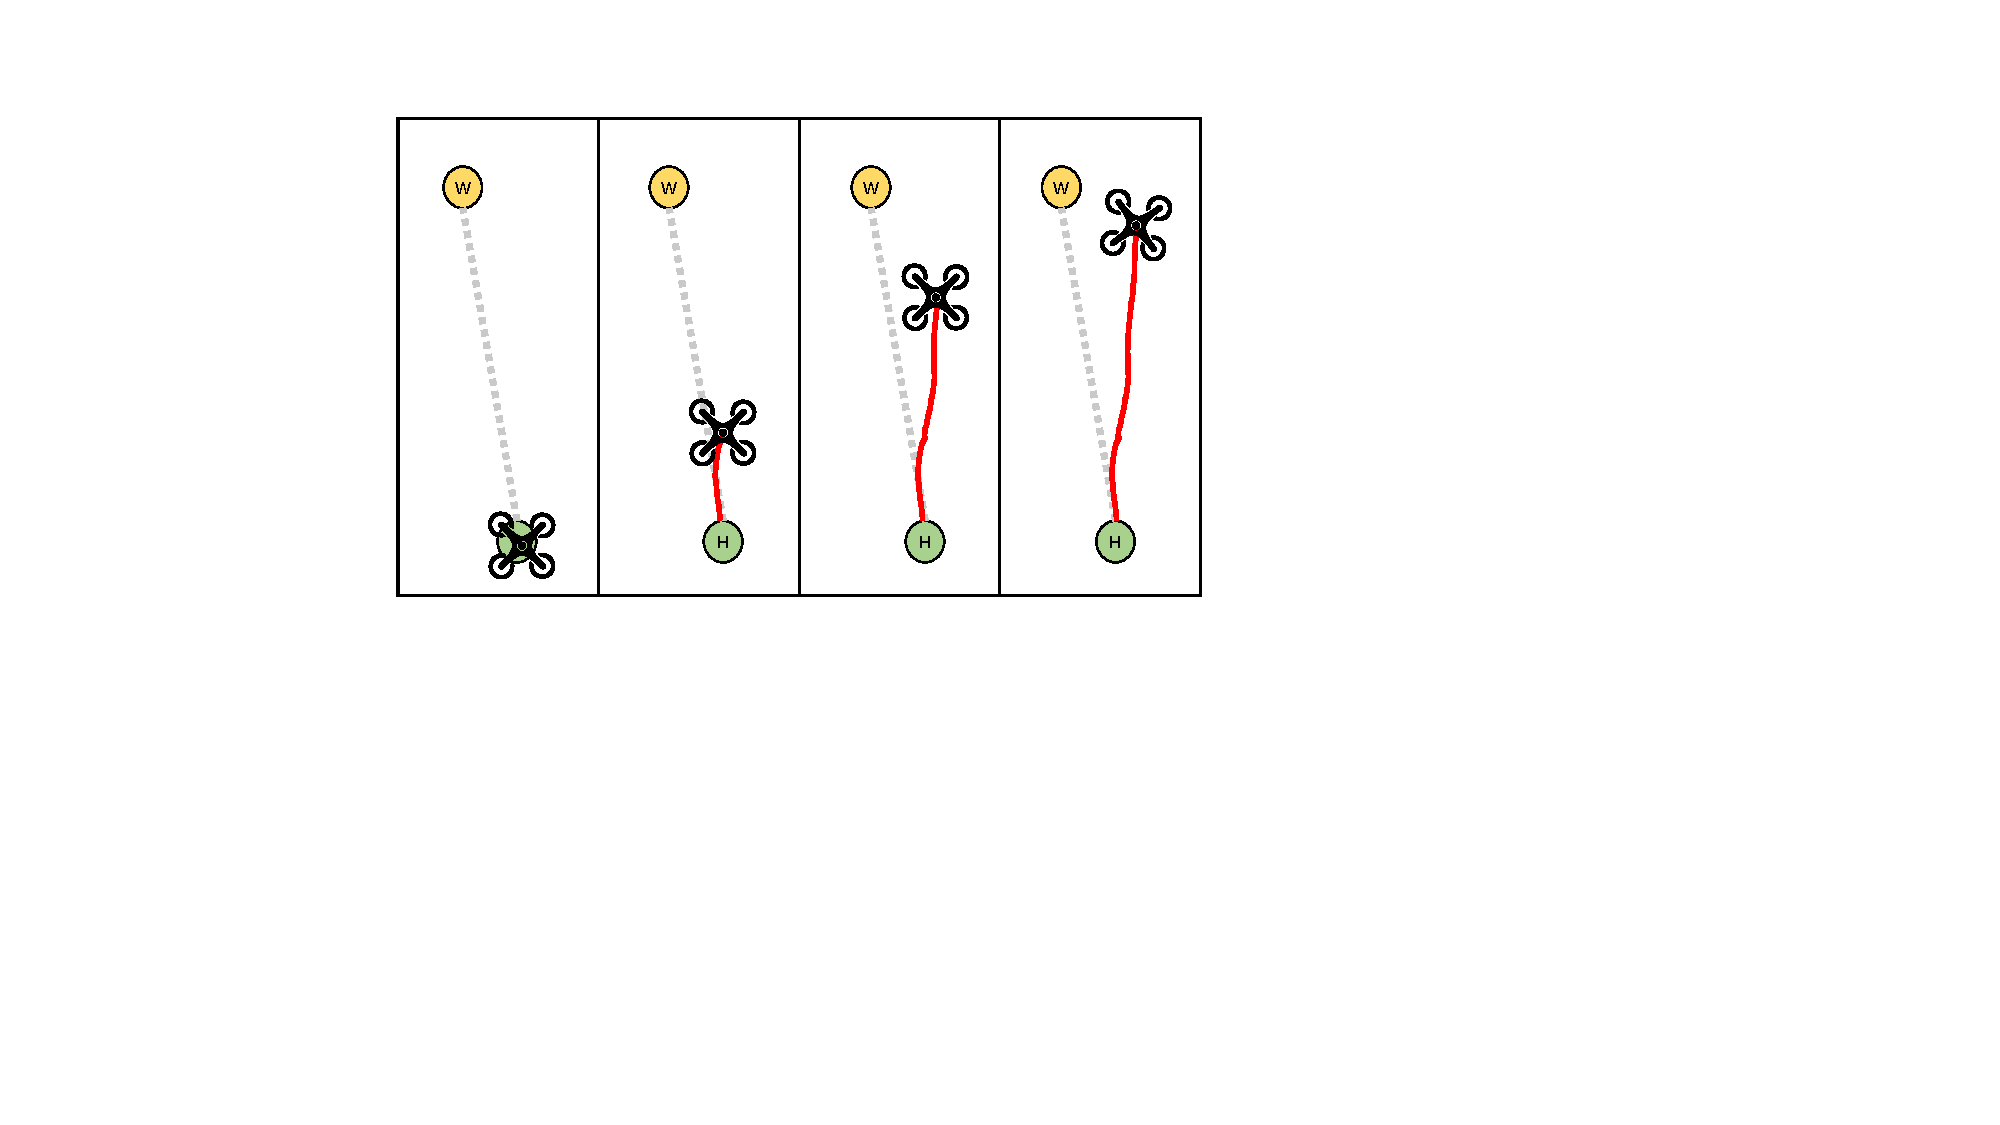
\includegraphics[width=0.48\linewidth]{fig/fix/unstable/deviation.pdf}
}
\subfloat[飞行冻结]{\label{subfig:exp_frozen}
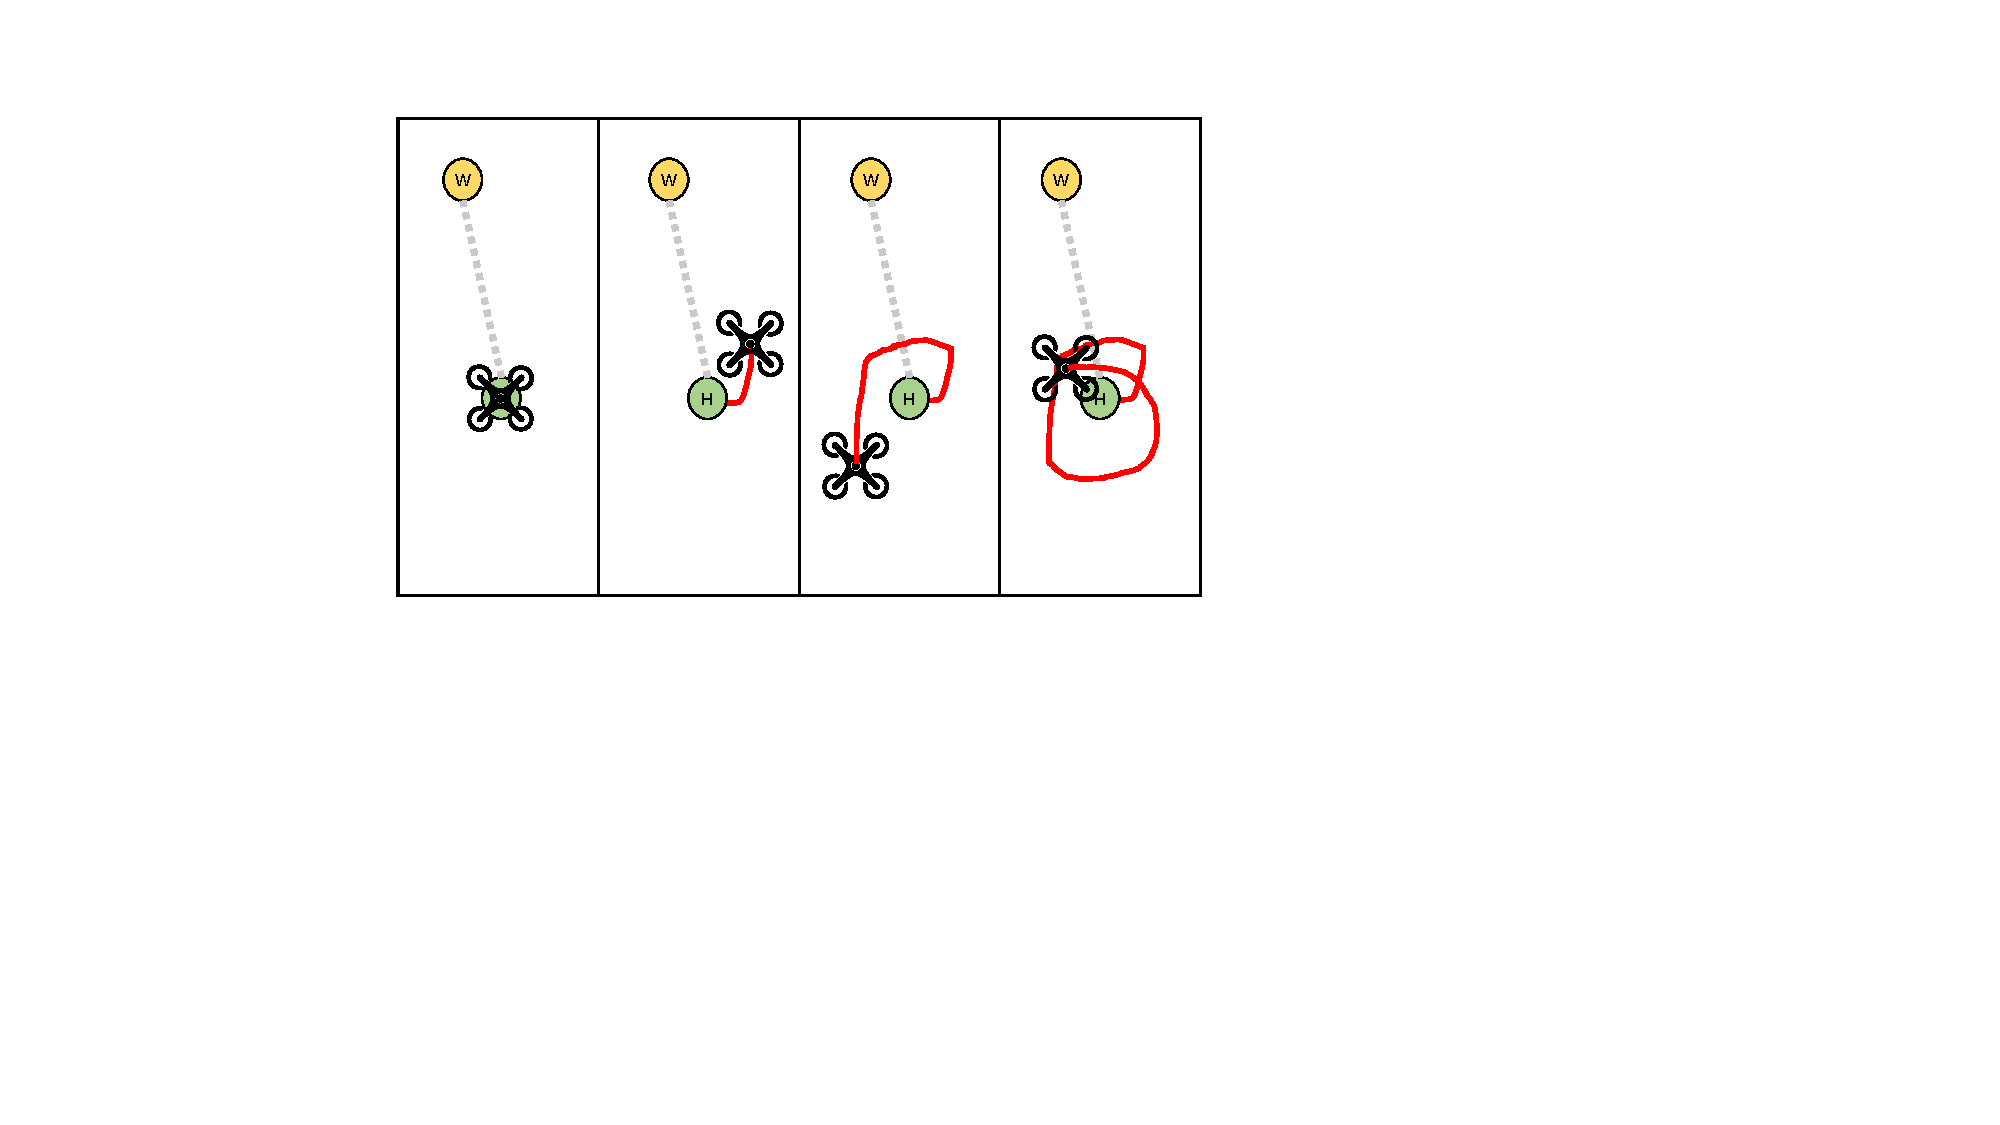
\includegraphics[width=0.48\linewidth]{fig/fix/unstable/frozen.pdf}}
}
\\
\subfloat[飞行坠毁]{\label{subfig:exp_crash}
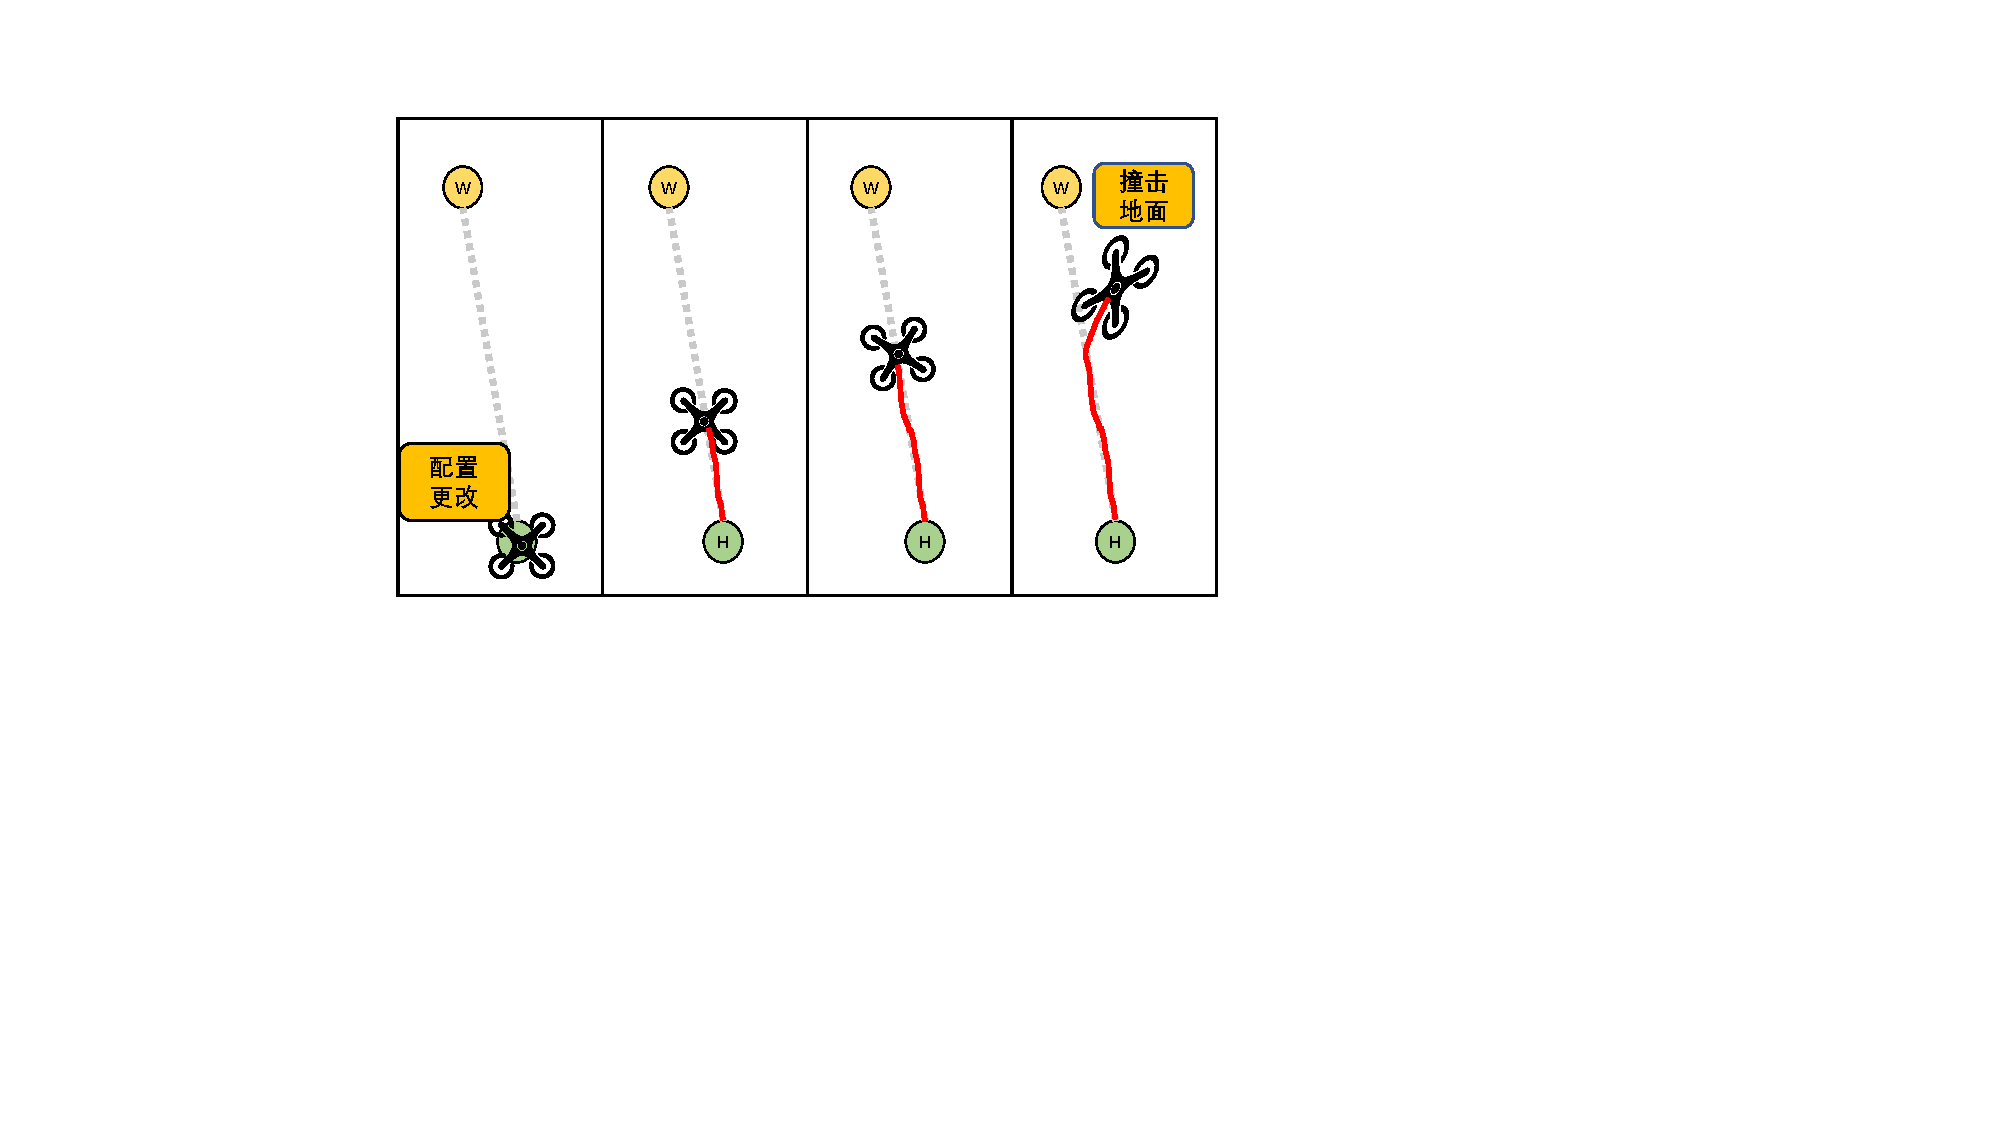
\includegraphics[width=0.48\linewidth]{fig/fix/unstable/crash.pdf}
}
\subfloat[动力损失]{\label{subfig:exp_thrust_loss}
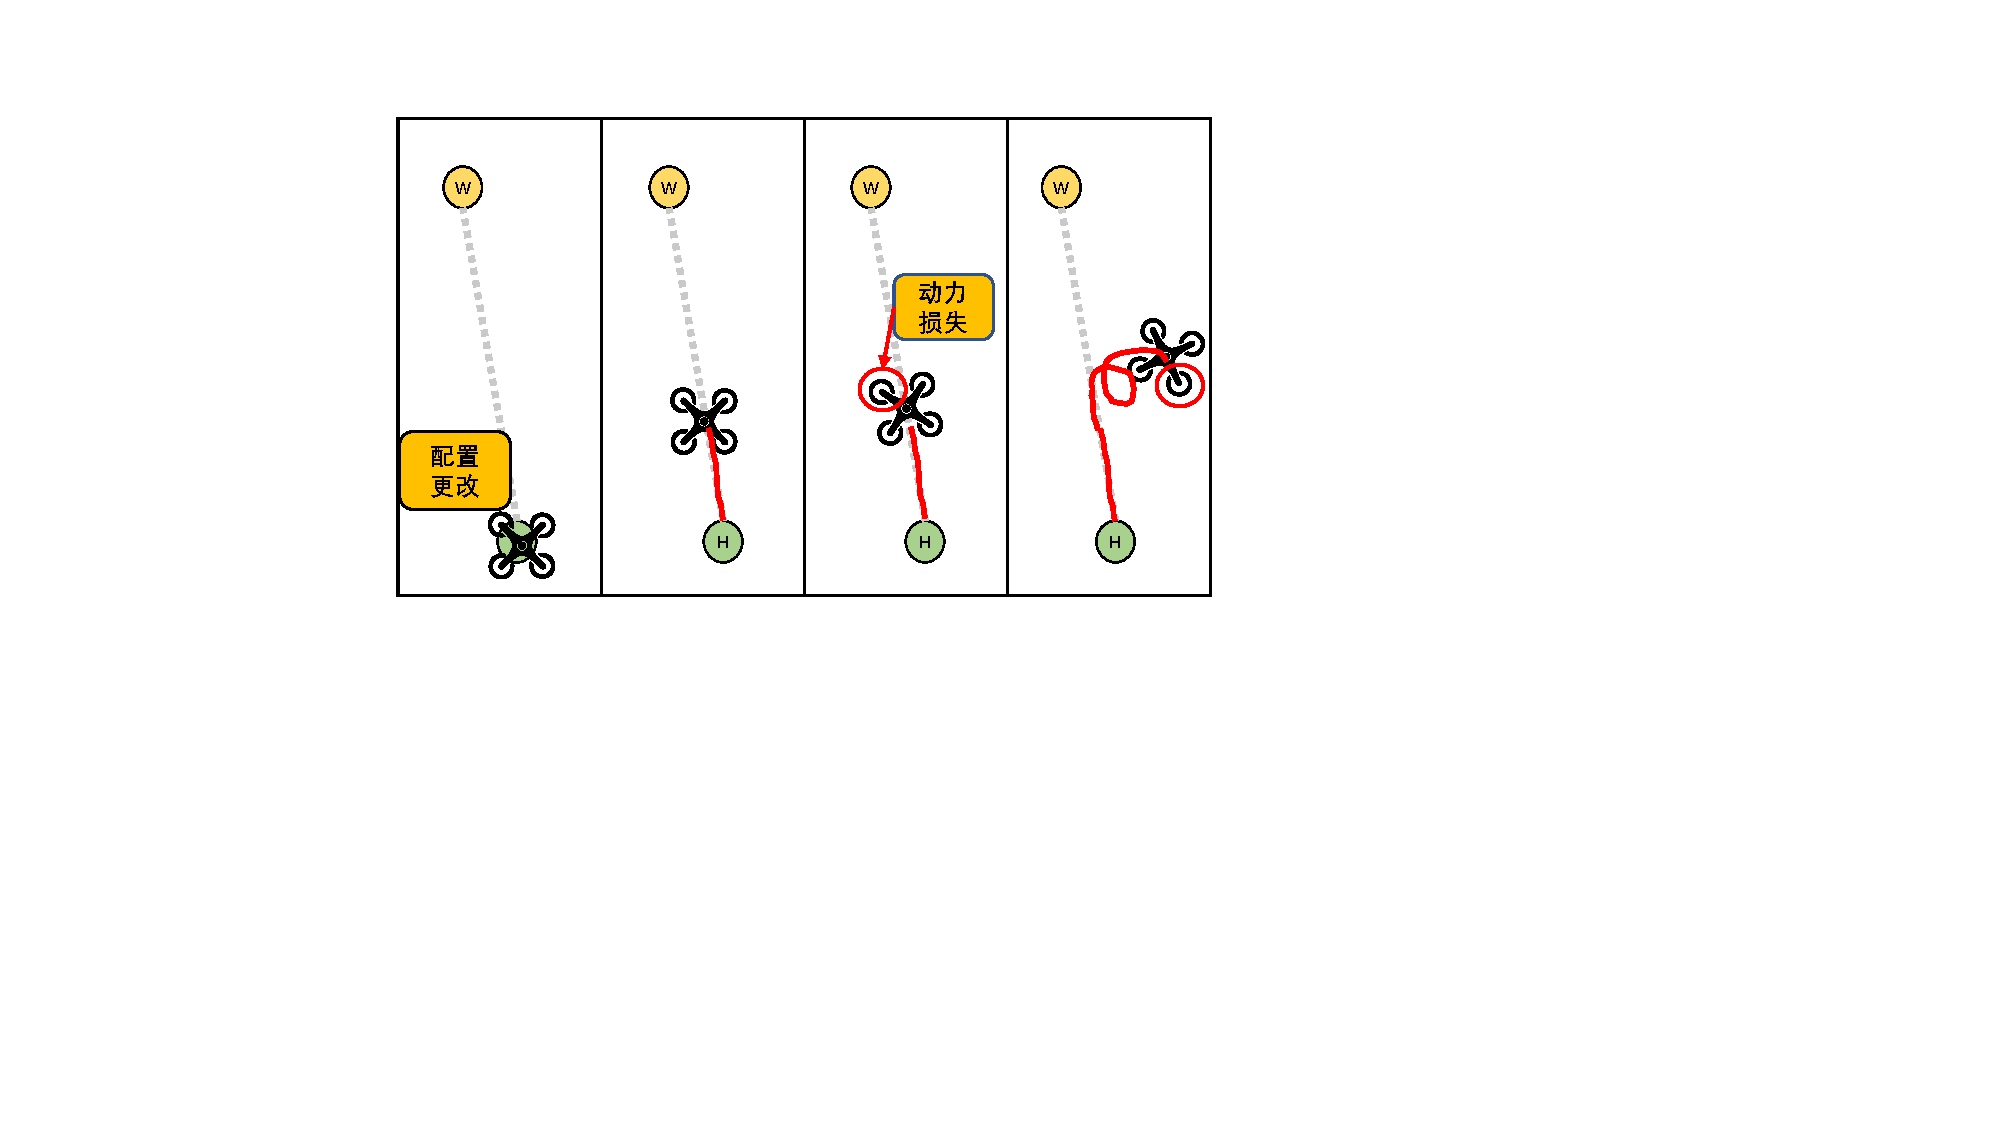
\includegraphics[width=0.48\linewidth]{fig/fix/unstable/thrust loss.pdf}}

\caption{四个不稳定物理状态示例的轨迹。}
\label{fig:unstable_example}
\end{figure}


\subsubsection{攻击下的状态变化}
为了更好地说明\dquote{如何评估和确定控制参数矫正的最佳时机},本预实验手动检查了攻击前后的状态变化,并记录了变化阶段。
以轨迹造成偏航的的配置攻击为例,图~\ref{fig:frozen_state} 分别展示了Roll、Pitch和Yaw角度变化的波动。

\begin{figure}[htb]
\centering{
\label{subfig:raw}
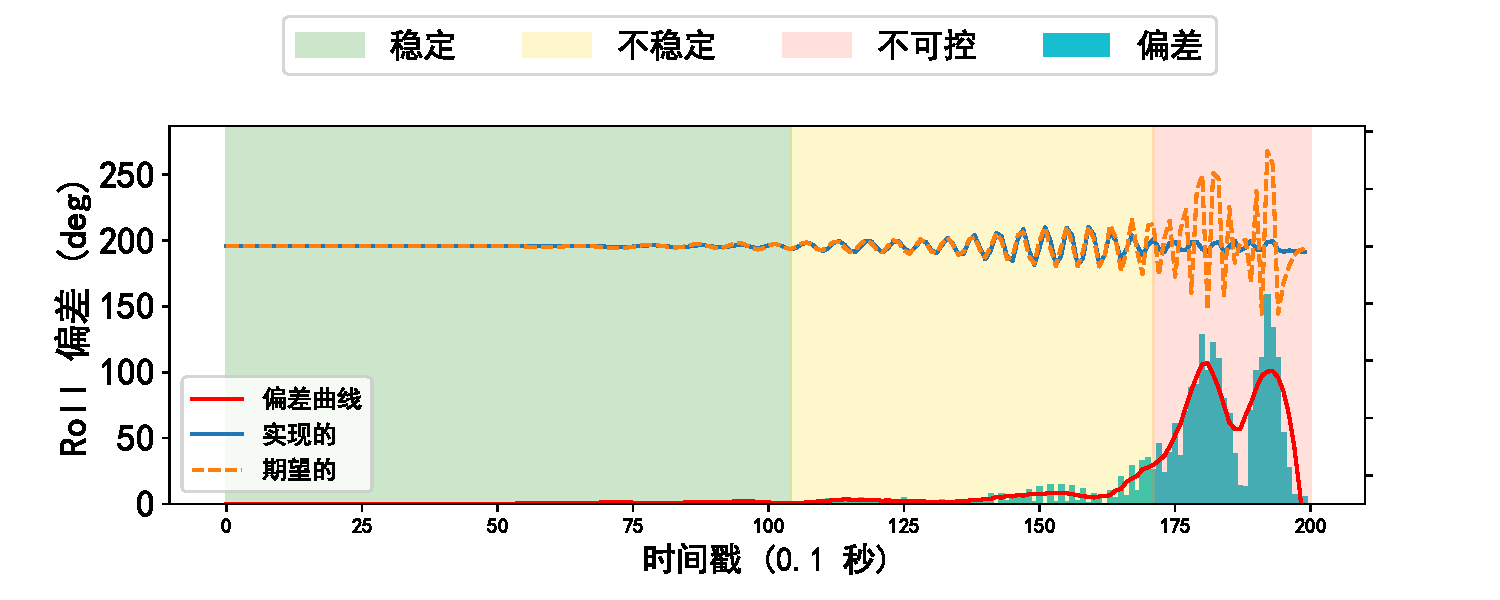
\includegraphics[width=0.88\linewidth]{fig/fix/unstable/frozen_states_roll.pdf} \\  
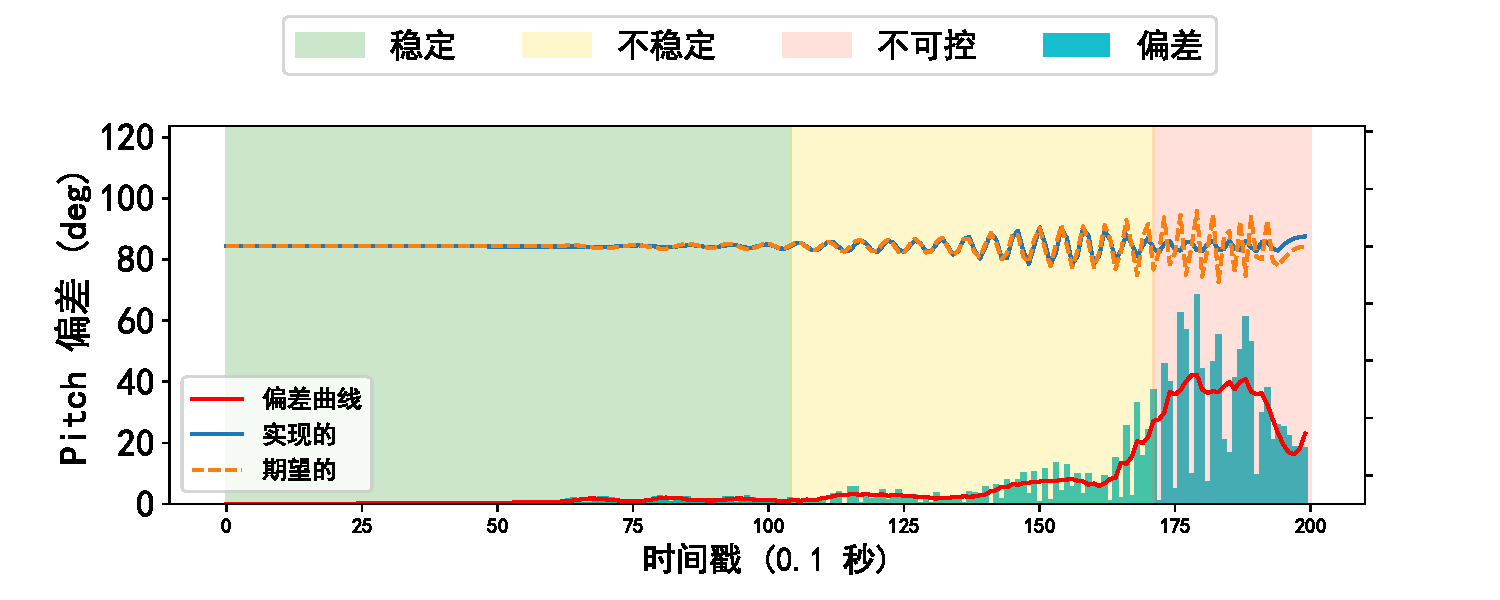
\includegraphics[width=0.88\linewidth]{fig/fix/unstable/frozen_states_pitch.pdf} \\
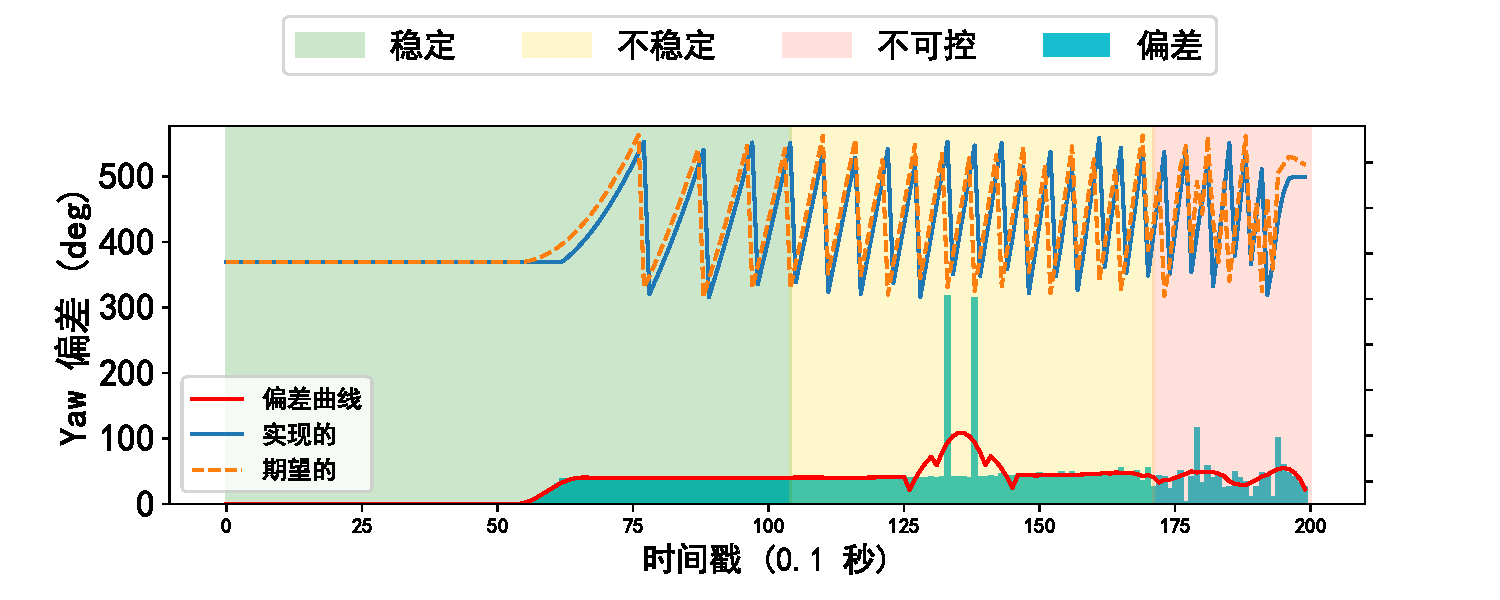
\includegraphics[width=0.88\linewidth]{fig/fix/unstable/frozen_states_yaw.pdf}
}
\caption{物理状态的角度变化}
\label{fig:frozen_state}
\end{figure}
根据偏差柱状图的观察结果,手动定义其三个阶段为:
\begin{itemize}
\item \textbf{0 to 10.3秒 (稳定)} 
在使用正常配置进行飞行任务时,无人机保持了稳定性。其每个状态下的现实的滚转、俯仰和偏航都符合预期,从图中也可以观察到,该阶段的偏差值都非常小,几乎可以忽略。


\item \textbf{10.4s to 17.1秒 (不稳定)}
无人机接收到不正确的配置后,其飞行姿态逐渐变得不稳定,表现出摇摆并且该阶段的偏差是逐渐增大的。
在这一阶段,无人机仍然按照正确的轨迹飞行,因为其自身的控制算法任然尝试矫正其飞行,但是已经出现了潜在的不稳定因素。
由于无人机仍然遵循着既定的飞行计划,这时仍然可以通过发送有效配置来矫正不稳定的物理状态,从而消除不利影响。


\item \textbf{17.2秒 之后 (不可控)}
随着这种不稳定因素的叠加,无人机已经无法正确的维持自身的飞行稳定,从而造成了较大的偏差。
图中显示的偏差也说明了混乱的状态。
飞行控制程序也检测到了不稳定状态,因为出现了明显的不稳定性和偏差,并报告了错误警告,且当前的飞行状态已经很难通过用户指令恢复正常。

\end{itemize}

观察结果表明,不正正确配置当在不稳定阶段中被发现并消除,这样无人机才能有恢复的可能。
因此,本节设计工具的目标是探索不稳定阶段,然后进行控制参数矫正,以矫正不稳定状态。



\subsection{在线矫正的特点}
对于范围规范错误,上一章的解决方案是在飞行前尽可能能让用户在安全的范围内选择参数配置。
但是相应的结果表明,这不能完全的杜绝所有的不正确配置的情况,尤其实在有外部攻击可能性的情况下,用户更加却反应对措施。
因此,在有上一章节的范围指南的情况下,依旧需要引入动态的飞行矫正方案,能够高效的解决飞行中突发攻击的防御场景,全方位的保障飞行安全。

而飞行中对参数进行矫正有以下挑战。

\begin{itemize}
    \item \textbf{挑战 1:不同飞控程序中控制参数设计及参数取值范围不一致。}
    由于缺乏统一的行业标准,制造商可以利用不同的控制参数元素将不同的功能合并到他们的飞行控制程序中。
    即使对于实现相同目标的参数元素,制造商可能会使用不同的参数名称。、
    此外,具有相同功能的参数的取值范围在不同的飞行控制程序中也可能不同。
    表~\ref{tab:fix_dis_params} 展示了两个流行的飞控程序\tool{Ardupilot}和\tool{PX4}中参数的比较。
    两个飞行控制程序都包含 2000 多个参数,但只有 249 个实现相同的功能。
    此外,每个飞行控制程序都有大约 100 个控制姿态相关控制参数,但只有 37 个(35\%)实现相同的功能。

    \begin{table}[ht]
\caption{不同控制程序中的参数(有范围限制的参数)}
\label{tab:fix_dis_params}
\centering
\begin{tabular}{c|cc}
        \toprule[1.5pt]
        ~ & \tool{Ardupilot} & \tool{PX4} \\
        \midrule[0.8pt]
        总计 & 2,990 & 2,407 \\
        \midrule[0.8pt]
        \makecell[c]{完全相同} & \multicolumn{2}{c}{66}  \\

        \makecell[c]{功能和范围相同} & \multicolumn{2}{c}{16}  \\

        \makecell[c]{仅功能相同} & \multicolumn{2}{c}{249}  \\
        
        \midrule[1.5pt]

        姿态相关的参数 & 105(3.5\%) & 101(3.5\%) \\
        \midrule[0.8pt]
         \makecell[c]{完全相同} & \multicolumn{2}{c}{0}  \\

        \makecell[c]{功能和范围相同} & \multicolumn{2}{c}{0}  \\

        \makecell[c]{仅功能相同} & \multicolumn{2}{c}{37}  \\
        
        
        \bottomrule[1.5pt]
\end{tabular}
\end{table}
   
    \item \textbf{挑战 2:控制参数之间相互依赖复杂,实时选择合适的配置较为困难。}
    控制参数的相互依赖性错综复杂地交织在一起,因为无人机中的所有组件都具有较高的关联性~\cite{ding2023get}。
    因此,有效管理这些依赖关系对于正确设置配置和消除不正确导致的不稳定至关重要。
    但是,与控制参数相关的初始化和范围检查代码通常是独立实现的,并且不考虑参数之间的相互依赖性。
    与起飞前测试的方式不同的是,在飞行过程中几乎没有可能考虑控制参数的如此复杂的值组合。
    因此测试所有组合(即配置)是不可行的。
    
    
    \item \textbf{挑战 3:配置受到不确定性执行环境的影响,产生意想不到的副作用。}
    由于执行环境的开放性,由配置产生的飞行状态的性能可能与预期的不同。
    虽然一些研究方法试图通过建立先验知识来描述潜在的执行条件来处理这种环境不确定性,尽管可以正确实施和设置与姿态相关的控制参数,很难估计现实中无人机飞行时的环境变化及其对姿态相关参数的影响。
     
\end{itemize}

\subsection{解决方案}
基于上述研究,稳健的控制参数矫正机制必须满足以下要求:

\begin{itemize}
\item \textbf{即时控制参数矫正:}
通过先前状态变化的样例可以发现大多数威胁首先导致无人机进入不稳定(但并非无法控制)的物理状态。
对此,如果发现不稳定的物理状态并及时生成新的控制参数配置,飞控程序就有足够的时间做出响应并重新驾驶无人机进入预期状态。
此外,多项研究~\cite{choi2020cyber,zhou2022doublestar}表明,某些入侵方法会持续攻击无人机,因此,不是在无人机起飞之前进行各种检查或者限制,而是在整个飞行过程中,矫正也应该持续进行,以保护控制参数 。


\item 
\textbf{自适应矫正:}
由于许多无人机不提供其控制程序的源代码且参数的名称和功能没有统一的规则,因此应用替代控制算法~\cite{choi2020software,dash2021pid}来增强原始飞行系统是不可行的。
可行的是,现在大多数无人机都提供配置调整接口,并且制造商通常会发布相应的手册来提供帮助。
因此,利用原生的控制参数配置接口来帮助无人机调整物理状态,相比需要重新编译原始无人机系统的解决方案要方便得多。
此外,由于这种设计使用的是无人机自身提供的内部机制,因此可以应用到不同的飞行控制程序中。

\end{itemize}

\section{方案}
本节介绍\nyctea 的设计和实现。首先介绍其架构的概述,然后详细讨论。

\subsection{概览}

\begin{figure*}[htb]
  \centering
    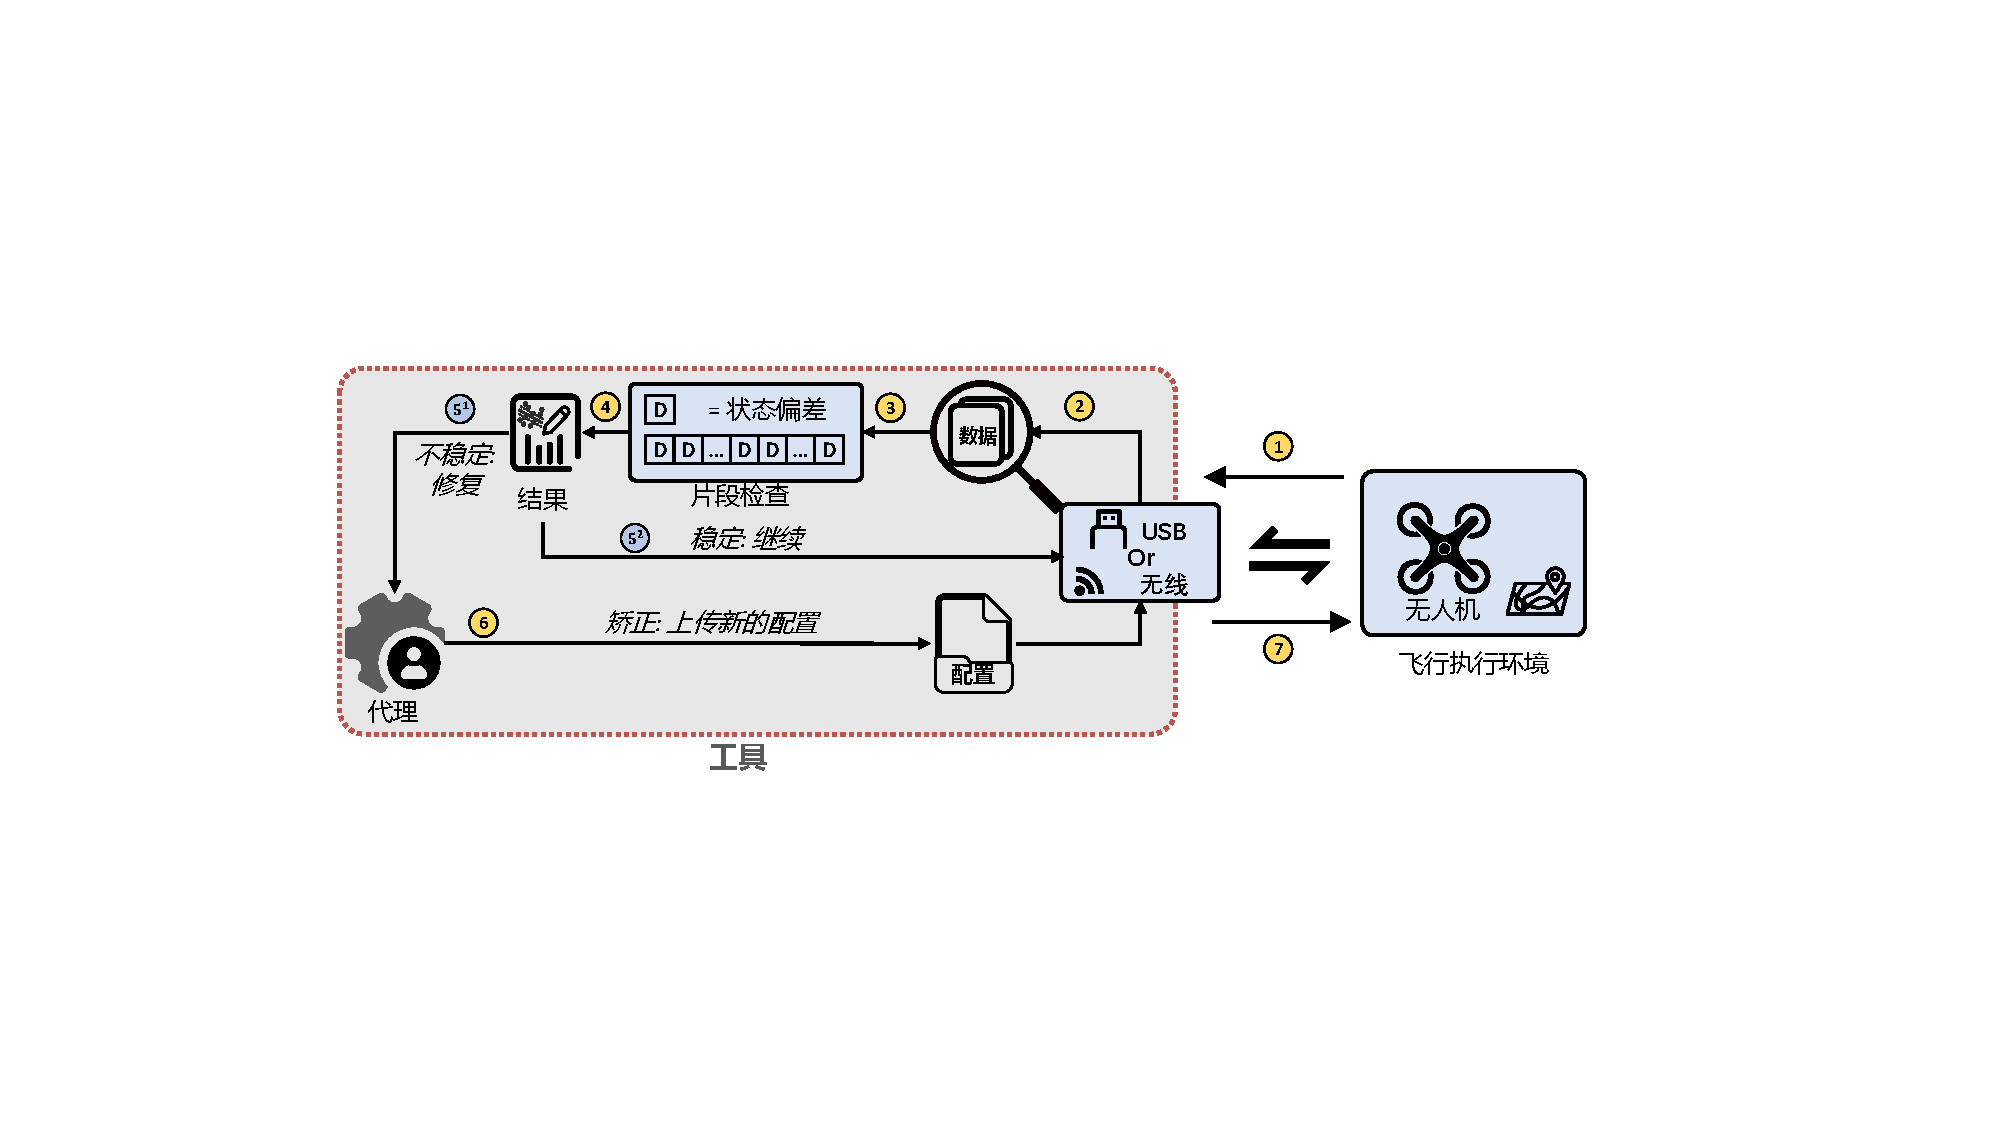
\includegraphics[width=\linewidth]{fig//fix/overview_fix.pdf}
\caption{\nyctea 架构概览}
\label{fig:fix_overview} 
\end{figure*}

\nyctea 的架构如图~\ref{fig:fix_overview} 所示。
\nyctea 利用无线或USB与无人机连接。 (\circled{1})。
它使用动态监控方法,利用段状态来跟踪无人机物理状态的变化(\circled{2}\circled{3})。
一旦获得段,\nyctea 就会计算段中的期望状态和实现状态之间的偏差 (\circled{4})。
如果所有状态偏差的总和低于预定义的阈值,\nyctea 会继续监视下一段 (\circled{$5^2$})。
否则,\nyctea 认为无人机具有不稳定的物理状态 (\circled{$5^1$}),并通过智能体模型创建配置来调整其飞行 (\circled{$6$})。
该过程是迭代的,\nyctea 捕获段偏差并实时矫正无人机。
下面首解释如何在\emph{飞行与校正建模}中对校正问题进行建模,如何进行\emph{智能体训练},以及在\emph{实时矫正}中的应用。


\subsection{飞行与校正建模}
矫正不稳定物理状态的问题可以从飞行物理稳定性的优化问题转换为奖励最大化问题,也就是什么样的配置能使当前状态获得最大的奖励(稳定性)。

\subsubsection{智能体状态}
为了有效地解决这个问题,本方案需要一个能够准确表示当前不稳定物理状态的智能体状态描述。 
该描述应捕获已实现的飞行状态与期望状态之间的偏差,使智能体能够生成适当的动作(即配置)作为响应。
考虑到不稳定状态的性质,智能体状态描述需要同时考虑无人机的物理状态和相应的传感器测量数据。

无人机在飞行过程中实时生成飞行日志数据。
\nyctea 通过生成片段来预处理飞行数据以供进一步分析。
在每个时间戳$t$,\nyctea 分别检索物理飞行状态$a_t$、期望飞行状态$a'_t$。
由于无人机可以完成360度翻滚, 此处物理和期望的飞行状态值被记录为基于弧度的。
此外,\nyctea 从陀螺仪和加速度计测量中获取相应的传感器数据 $e_t$。
在时间戳 $t$ 捕获的每个航班数据可以用一个三元组表示,即 $s_t = \{a_t, a'_t, e_t\}$。
\nyctea 收集连续的飞行数据形成一段$S$来探索偏差变化。
一个段,记录从时间戳$t$收集的数据,表示如下:
\begin{equation}
    S_t = \{s_j~|~j \in [t, t+m_{3}-1]\}
\end{equation}
其中$m_{3}$是段的长度。

\subsubsection{不稳定监测}
对于分段,系统通过检查期望状态和物理状态之间的分段偏差是否超出可接受的范围来监控无人机的不稳定性。
$S_t$ 段中的物理状态和期望状态为:
\begin{equation}
\begin{aligned}
    A_t = \{~a_j~|~j \in [t, t+m-1]~\}\\
    A'_t = \{~a'_j~|~j \in [t, t+m-1]~\}
\end{aligned}
\end{equation}
\nyctea 首先计算每个物理飞行状态与其相应的期望飞行状态之间的一范数:
\begin{equation}
d_j = ~\Vert~a_j - a'_j~\Vert, ~j \in [t, t+m-1]
\end{equation}
然后,\nyctea 通过对各个偏差 $Dv_t=\sum_{t}^{t+m-1}{d_j}$ 求和来计算分段偏差值 $Dv_t$。
如果 $Dv_i$ 大于阈值 $TH$,则 \nyctea 识别出不稳定状态(章节~\ref{subsec:fix_th_decided} 介绍了实验设置用于此阈值的值的方法),然后激活状态矫正器模块。否则,\nyctea 继续捕获并分析下一段。

\subsection{状态矫正}
当报告不稳定时,系统将段作为输入,并利用基于配置的控制方案来纠正状态以消除不稳定性。
整改过程使用预先训练的学习智能体,逐渐消除不稳定因素。

\subsubsection{动作空间}  
\nyctea 的目标是给出适当的动作(配置)来调整当前无人机来保持稳定。
动作空间可以定义为智能体可以采取的所有可能动作的集合。
对于本问题,动作空间$\mathbb{C}$被定义为所有可能的参数组合的集合,这些组合受到官方指南和规范的约束。
具体的动作(配置)$c$如下所示:
\begin{equation}
    c = \{~p'_1, p'_2, ..., p'_{n3}~\}, c \in \mathbb{C}
\end{equation}
其中 $p'$ 是新参数值,$n$ 是配置中的参数数量。

\subsubsection{动作模型训练}
\nyctea 训练一个参与者模型来生成用于纠正的配置,并根据制定的奖励函数增强模型。
训练执行了一架配置错误的无人机来完成飞行任务~\tool{AVC2013}~\cite{avc}。
在训练之前,\nyctea 利用之前的模糊测试工具,生成大量的不正确配置用于训练。
在每次执行最初使用其默认配置启动飞行控制程序。
然后在第一个航路点上传不正确配置。
随后启动\nyctea 中的智能体来进行矫正的修复。
它收集矫正经验并更新智能体,在后续检测到不稳定阶段时生成适当的配置。
\nyctea 通过深度强化学习策略\tool{(Deep Deterministic Policy Gradient,DDPG)}~\cite{lillicrap2015continuous}来实现该目标,详细步骤见算法~\ref{alg:fix_system}。

\SetAlFnt{\small}
\begin{algorithm}[htb]
\caption{训练流程}\label{alg:fix_system}
 \LinesNumbered
 \KwIn{
训练批量尺寸 $N$, 软更新因子 $\tau$, 贴现系数 $\gamma$,
 不正确配置集 $ICs$, 偏差阈值 $TH$
 \;
 }
 初始Critic网络 $Q(\cdot)$, $Q'(\cdot)$\ 包含权重 $\theta^{Q}$, $\theta^{Q'}$\;
 初始Actor网络 $\mu(\cdot)$ and $\mu'(\cdot)$ 包含权重 $\theta^{\mu}$, $\theta^{\mu'}$\;
 最初, $\theta^{Q'} \gets \theta^{Q}$, $\theta^{\mu'} \gets \theta^{\mu}$\;
 重播缓冲区 $R$\;
 
\For{$ic_{k}$ in $ICs$}{
    初始化飞行场景 $ic_{k}$ 并启动\;
    \For{时间戳 $i$ in  执行($ic_{k}$)}{
      观察一个片段 $S_t$\;
      计算偏差 $Dv_t$\;
      \If{$Dv_t < TH$}{
        continue;
      }

      
      选择动作 $c_t \gets \mu(S_t)$\;
      $S_{next}$, $r_t$ $\gets$ 执行动作 $c_t$\;
      存储元组 $(S_t, c_t, r_t, S_{next})$ in $R$\;
    
      
      \If{$length(R) < N$}{
        continue;
      }
      随机批量 $N$ 个转换元组 $(S_j, c_j, r_j, S_{(j,next)}), j \in N$ from $R$\;
    
      计算 $y_j = r_t + \gamma Q'(r_j, \mu'(S_{(j,next)})$\
      
      通过最小化损失来更新批评家 (\ref{eq:loss})\;
      %$$L = \frac{1}{N}\sum_{j}(y_j - Q(S_j, c_j))^2$$\

      使用采样的策略梯度更新参与者策略 (\ref{eq:policy})\;

      % $$\nabla_{\theta^{\mu}} \approx \frac{1}{N} \sum_{j}\nabla_{c}Q(S,c)\mid_{S=S_j, c=\mu(S_j)}\nabla_{\theta^{\mu}}\mu(S)\mid_{S_j}$$

      更新网络 (\ref{eq:sigma})\;
      % $$\theta^{Q'} \gets \tau \theta^{Q} + (1-\tau)\theta^{Q'}$$
      % $$\theta^{\mu'} \gets \tau \theta^{\mu} + (1-\tau)\theta^{\mu'}$$
      
     }
}

 
\end{algorithm}


最开始,\nyctea 设置了一些初始化因素,包括训练批量大小$N$、模型软更新因子 $\tau$、学习折扣因子 $\gamma$、偏差值阈值 $TH$(将在章节~\ref{subsec:fix_th_decided}中决定)和重播缓冲区$R$。
\nyctea 还初始化Critic网络$Q(\cdot)$、$Q'(\cdot)$ 以及权重 $\theta^{Q}$、$\theta^{Q'}$\ 和Actor网络 $\mu (\cdot)$ 和 $\mu'(\cdot)$ 的权重为 $\theta^{\mu}$、$\theta^{\mu'}$。
最初的$\theta^{Q'}$和$\theta^{\mu'}$等于$\theta^{Q}$和$\theta^{\mu}$。

随后,应用生成大量的不正确配置集$IC$来进行训练。
\nyctea 发起启动飞行测试,然后在第一个航点上传一个不正确配置,它监视飞行日志数据(即姿态状态和传感器数据)并捕获段$S_t$数据(第 8 行)。
\nyctea 计算偏差值 $Dv_t$(第 9 行)。
如果偏差值低于阈值 $TH$,则 \nyctea 继续并捕获下一段。
否则,\nyctea 将这段 $S_t$输入到Actor网络$\mu(S_t)$中并获得一个动作(配置)$c_t$(第 13 行)。
随后,\nyctea 用这个新配置上传至无人机,观察下一段$S_{next}$,使用章节~\ref{subsec:fix_reward}中的方法计算奖励$r_t$(第 14 行)。
这一系列操作生成的元组$(S_t, c_t, r_t, S_{next})$将存储在重播缓冲区$R$中(第 15 行)。
如果重放缓冲区的大小超过设定的训练批量尺寸大小,\nyctea 会从历史经验中学习并相应地更新模型权重(第 19 到 23 行)。
具体而言,\nyctea 随机采样$N$个转换元组,每个元组为:
\begin{equation}
    (S_j, c_j, r_j, S_{(j,next)}), j \in [1, N]
\end{equation}
\nyctea 随后计算:
\begin{equation}
    y_j = r_t + \gamma Q'(r_j, \mu'(S_{(j,next)})
\end{equation}
\nyctea 通过最小化损失来更新Critic:
\begin{equation}\label{eq:loss}
    L = \frac{1}{N}\sum_{j}(y_j - Q(S_j, c_j))^2
\end{equation}
并使用采样的策略梯度更新参与者策略:
\begin{equation}\label{eq:policy}
    \nabla_{\mu} \approx \frac{1}{N} \sum_{j}\nabla_{c}Q(S,c)\mid_{S=S_j, d=\mu(S_j)}\nabla_{\theta^{\mu}}\mu(S)\mid_{S_j}
\end{equation}
经过一轮策略更新后,Actor和Critic网络权重被软更新:
\begin{equation}\label{eq:sigma}
    \begin{aligned}
        \theta^{Q'} = \tau \theta^{Q} + (1-\tau)\theta^{Q'} \\
        \theta^{\mu'} = \tau \theta^{\mu} + (1-\tau)\theta^{\mu'}
    \end{aligned}
\end{equation}

其中特殊的情况是,如果无人机在飞行过程中触发严重不稳定或成功着陆,任务将重新开始,但重播缓冲区将保留。
一旦无人机能够连续三次矫正当前的不正确配置(无人机成功完成任务),训练就会进入其他实验攻击场景。
最后,在学习过程结束时,使用智能体的Actor网络 $\mu$ 来生成校正。


\subsubsection{奖励函数}\label{subsec:fix_reward}
对于智能体状态 $S_t$,\nyctea 会计算偏差值$Dv_t$。
然后通过智能体的Actor$\mu(\cdot)$来根据此状态生成一个操作(即配置$c_t$)并将其上传到无人机:
\begin{equation}
    c_t = \mu(S_t)
\end{equation}
\nyctea 观察下一个智能体状态$S_{next}$作为此操作的结果,并以相同的方式计算下一个偏差值$Dv_{next}$。
偏差变化$Dc$计算为先前偏差值和新偏差值之间的差:
\begin{equation}
    Dc_t = Dv_{next} - Dv_t
\end{equation}
根据 $Dc_t$ 值,\nyctea 采用不同的策略给予奖励:

\begin{itemize}
    \item \textbf{正值:} 如果偏差值$Dv_t>0$, 此训练过程并不会直接使用该偏差值作为奖励。
    \nyctea 设计的整体目标是生成的配置需要尽可能的将一个无人机飞行状态从一个较大的偏差减少到较小的偏差,也就是从不稳定变化到更稳定。
    即使中间出现较大额偏差缩减,但是缩减后的偏差没有保持一个较小的值的话,也不应获得较大的奖励。
    而通过矫正配置后的偏差$S_{next}$越接近于零,则配置会应该收到更大的奖励。
    相反,即使$Dc_t$有较大的偏差变化,但是下一个偏差值$Dv_{next}$不接近于零(足够稳定),配置也不应获得更大的奖励。
    除此之外,智能体可能会为了追求高奖励而生成过于极端的配置,例如允许无人机在飞行中悬停并达到较小的下一个偏差值$Dv_{next}$,这会导致无人机无法继续完成任务,与修复目标本身相违背。
    为了防止这种情况,\nyctea 将最小值$Dv_{next}$设置为1,即 $max(1, Dv_{next})$并将$Dc_t$乘以一个加速比例$acc_t$。
    该加速比例为矫正配置造成给下一时刻$S_{next}$中的平均加速度。
    在该加速度比例的影响下,如果矫正配置是的无人机的动作变化太小,则相应的奖励权重将会变小。
    总体上讲,所设计的正值奖励计算方式如下:
    \begin{equation}
        r_t = \frac{Dc_t * acc_t}{max(1, Dv_{next})}
    \end{equation}

    下面将通过一些例子说正值奖励的处理过程。
    假设配置将偏差从$80$减少到$20$,造成的下一个时刻数据片段的加速比例为$1.2$。
    此时前后两个片段数据产生的偏差变化为$60$。
    虽然这个偏差减少量不算少,但是由于下所造成的片段状态(偏差为$20$)仍然不稳定。
    \nyctea 认为这种配置有一些积极作用,但不足以获得更大的奖励。
    因此,它只能获得$\frac{60*1.2}{20}=3.6$奖励。
    假设另一种配置以$0.8$的加速比例将偏差从$20$减少到$1$,则它可以获得$\frac{20*0.8}{1}=16$的更高奖励,因为作为其后续片段(偏差值为$1$)更稳定。
    令一种极端的情况是,假设配置将偏差从$80$减少到$20$,但加速比例为$0.1$,也就是以为着无人机几乎停止移动。
    它只收到$\frac{60*0.1}{20}=0.3$奖励。

    \item \textbf{负值:} 如果偏差值$Dv_t<0$, 训练过程会对该配置进行惩罚。
    即使智能体生成的配置不能充分减轻偏差,该配置也不应该进一步加剧不稳定性,也就是增加偏差。
    因此,如果偏差值$Dc_t$为负,则\nyctea 直接使用偏差变化值$Dc_t$作为奖励。
    例如,假设配置将偏差值从$20$加剧到了$30$,智能体将收到$30-20 = -10$的奖励。
    

    \item \textbf{严重不稳定或特殊情况:}     
    如果配置直接触发失控(例如,坠毁、推力损失和无法控制的飞行的轨迹偏差),\nyctea 将负面奖励加倍作为惩罚形式。
    也就是说,即使该配置稳定了无人机,但导致了严重的事件,例如稳定后方向错误(轨迹偏差),也不会得到积极的奖励。
    
\end{itemize}


\subsection{实时矫正}
一旦进入失控阶段,无人机可能会出现极大的偏差,无法矫正飞行。
为了防止这种情况发生,\nyctea 会检测不稳定的物理状态并启动适当的配置。
\nyctea 不断捕获飞行段数据$S$并计算偏差值$Dv$。
参考检测阈值$TH$,如果偏差值超过阈值,则\nyctea 将使用不稳定标签标记捕获的片段。
然后,\nyctea 将当前段$S$输入到智能体中,并获取用于更新无人机的新配置。
如果下一个观察到的偏差仍然超过阈值,则继续矫正。

\section{实验结果及分析}

本章节通过检测精度和矫正成功率方面评估\nyctea 的性能,同时还分析误报和时间消耗。
\begin{itemize}
 
\item \textbf{研究问题1 识别准确率:} \nyctea 能否实时有效识别不稳定因素?

\item \textbf{研究问题2 矫正性能:} \nyctea 能否消除不稳定因素,成功防范潜在威胁? 涉及的控制参数数量是否影响整改成功率?

\item \textbf{研究问题3 时间消耗:}\nyctea 需要多长时间才能生成配置并最终消除不稳定因素?

\end{itemize}
\subsection{实验准备}

\subsubsection{实验设定}

\begin{itemize}
    \item \textbf{实验程序:}
实验主要在两个流行的飞行控制程序 \tool{ArduPilot} (4.2.0)~\cite{ardupilot} 和 \tool{PX4} (1.13)~\cite{px4} 上测试了 \nyctea。
此处的实现使用 \tool{Mavlink}~\cite{mavlink} 将 \nyctea 与 \tool{Ardupilot} 和 \tool{PX4} 连接,并调用第三方包的函数\tool{Pymavlink}~\cite{pymavlink} 用于数据捕获和配置上传。
由于实验硬件以10Hz将内存数据写入闪存,因此采用统一的采样率10Hz,也就是数据采集间隔是$0.1s$。
根据手动测试,飞行控制程序通常需要两秒以上才能对不正确做出反应。
因此,本实验中的片段通过连续捕获两秒的数据形成。
鉴于 \nyctea 每 $0.1s$ 捕获一次飞行数据,每轮分析涉及一个大小为$20$的数据片段。
关于智能体设置,本实验将缓冲区的最大容量设置为 $20,000$,软更新因子为 $0.02$,折扣因子为 $0.99$,批量大小为 $64$。
Actor和Critic的网络具有相同的网络结构,其中包含三个隐藏大小为256的线性层。

\item \textbf{测试设备:}
由于不稳定可能会导致无人机遭受物理损坏以及涉及行人的潜在事故的风险,实验使用模拟器进行了大部分实验。
使用配备\tool{Ardupilot}的\tool{APM}和配备\tool{PX4}的\tool{Jmavsim}。
对于一些导致较小风险的测试用例,实验将这些案例集成到配备\tool{Ardupilot}的物理无人机\tool{CUAV ZD550} 中,以评估工具在现实场景中的性能。

\item \textbf{参数选择:}
每个飞行控制程序由数百个参数组成,但其中只有少数参数与飞行调整和稳定性密切相关。
因此,实验根据官方手册提供的控制参数说明,选择了与角姿态和角速率相关的参数。
如表~\ref{tab:fix_param_both}所示,实验从\tool{Ardupilot}中选择了$17$参数,从\tool{PX4}选择了$11$参数。

% \begin{table}[ht]
% \small
% \caption{Parameters for experiments.}
% \label{tab:param_both}
% \centering
% \begin{tabular}{c|c}
%         \toprule[1.5pt]
%         \textbf{Ardupilot} & \textbf{PX4}\\
%         \midrule[0.8pt]
%     \makecell*[c]{PSC\_VELXY\_P\\PSC\_VELXY\_I\\PSC\_VELXY\_D\\PSC\_ACCZ\_P\\PSC\_ACCZ\_I\\ATC\_ANG\_RLL\_P\\ATC\_RAT\_RLL\_P\\ATC\_RAT\_PIT\_I\\ATC\_RAT\_RLL\_D\\ATC\_ANG\_PIT\_P\\ATC\_RAT\_PIT\_P\\ATC\_RAT\_PIT\_I\\ATC\_RAT\_PIT\_D\\ATC\_ANG\_YAW\_P\\ATC\_RAT\_YAW\_P\\ATC\_RAT\_YAW\_I\\ATC\_RAT\_YAW\_D\\} 
%     & 
%     \makecell*[c]{ MC\_ROLL\_P\\MC\_PITCH\_P\\MC\_YAW\_P\\MC\_YAW\_WEIGHT\\MPC\_XY\_P\\MPC\_Z\_P\\MC\_PITCHRATE\_P\\MC\_ROLLRATE\_P\\MC\_YAWRATE\_P\\MPC\_TILTMAX\_AIR\\MPC\_TKO\_SPEED} \\
%     \bottomrule[1.5pt]
% \end{tabular}
% \end{table}

\begin{table}[ht]
\small
\caption{实验参数}
\label{tab:fix_param_both}
\centering
\begin{tabular}{c|c|c}
\toprule[1.5pt]
\textbf{参数描述}      & \textbf{Ardupilot} & \textbf{PX4}          \\ 
\midrule[0.8pt]
Roll angle P gain         & ATC\_ANG\_RLL\_P   & MC\_ROLL\_P           \\ \hline
Pitch angle P gain        & ATC\_ANG\_PIT\_P   & MC\_PITCH\_P          \\ \hline
Yaw angle P gain          & ATC\_ANG\_YAW\_P   & MC\_YAW\_P            \\ \hline
Roll rate P gain          & ATC\_RAT\_RLL\_P   & MC\_ROLLRATE\_P       \\ \hline
Pitch rate P gain         & ATC\_RAT\_PIT\_P   & MC\_PITCHRATE\_P      \\ \hline
Yaw rate P gain           & ATC\_RAT\_YAW\_P   & MC\_YAWRATE\_P        \\ \hline
Roll rate I gain          & ATC\_RAT\_RLL\_I   &                       \\ \hline
Roll rate D gain          & ATC\_RAT\_RLL\_D   &                       \\ \hline
Pitch rate I gain         & ATC\_RAT\_PIT\_I   &                       \\ \hline
Pitch rate D gain         & ATC\_RAT\_PIT\_D   &                       \\ \hline
Yaw rate I gain           & ATC\_RAT\_YAW\_I   &                       \\ \hline
Yaw rate D gain           & ATC\_RAT\_YAW\_D   &                       \\ \hline
Velocity P gain           & PSC\_VELXY\_P      &                        \\ \hline
Velocity I gain           & PSC\_VELXY\_I      &                        \\ \hline
Velocity D gain           & PSC\_VELXY\_D      &                        \\ \hline
Acceleration P gain.      & PSC\_ACCZ\_P       &                        \\ \hline
Acceleration P gain.      & PSC\_ACCZ\_I       &                        \\ \hline
Yaw weight                &                    & MC\_YAW\_WEIGHT       \\ \hline
Horizontal error gain     &                    & MPC\_XY\_P            \\ \hline
Vertical error gain       &                    & MPC\_Z\_P             \\ \hline
Maximum tilt angle        &                    & MPC\_TILTMAX\_AIR     \\ \hline
Takeoff climb rate        &                    & MPC\_TKO\_SPEED       \\ 
\bottomrule[1.5pt]
\end{tabular}
\end{table}



       

\end{itemize}


\subsubsection{配置数据集构造}
为了评估 \nyctea 的性能,实验首先构建了一个包含安全配置和不正确配置以及相应飞行状态的配置数据集。
实验使用\tool{LGDFuzzer}~\cite{han2022control} 来探索潜在的安全配置和不正确。
然后通过将这些配置输入飞行模拟器来执行飞行任务\tool{AVC2013}~\cite{avc},这些飞行任务的第一个航路会有意地点引入不正确配置。
最后,实验过程中会使用利用 \tool{PyMavlink} 来检查每个飞行任务是否成功完成。
如果一个飞行测试中无人机顺利降落,则该测试配置被确认为 \dquote{安全}; 否则,被认为是\dquote{不正确配置}。

通过实验观察发现配置会导致飞行状态下的不同的无人机错误报告:
\begin{itemize}
\item 执行器相关错误(AR):它导致飞行控制程序报告与执行器相关的警告,例如潜在的推力损失、油门错误、偏航不平衡和碰撞。

\item 任务执行错误(ME):使飞行轨迹偏离预期路径,如轨迹偏离、飞行悬停等。

\item 系统故障保护错误(SF):导致飞控程序报告故障保护,例如EKF故障保护(位置和姿态估计系统不健康)和传感器故障保护(传感器测量值不一致)。

\end{itemize}

实验总共对\tool{Ardupilot}控制程序收集了6,545个配置,包括 1,781 个安全配置和4,764个不正确,以及对\tool{PX4}收集了4,829 个配置,其中包括 1,367 个安全配置和 3,462个不正确。
由于\nyctea 需要阈值 $TH$ 来确定无人机的稳定性,并依赖智能智能体来生成正确的配置,实验将数据集分为训练集和测试集。
训练集用于确定阈值并训练智能体,而测试集用于评估系统。
具体来说,实验分别在\tool{Ardupilot}和\tool{PX4}中随机选择了1,000个安全配置,并分别从\tool{Ardupilot}和\tool{PX4}中选择了2,785和2,228个不正确。
数据集详细信息列于表~\ref{tab:fix_unstable_env} 中。

\begin{table}[ht]
\caption{测试场景分布}
\label{tab:fix_unstable_env}
\centering
\begin{threeparttable}
\begin{tabular}{c|cccc}
        \toprule[1.5pt]
        ~ & {\makecell*[c]{安全}}  & {\makecell*[c]{执行器相关}} & {\makecell*[c]{任务执行}} &  {\makecell*[c]{系统故障保护}} \\
        
        \midrule[0.8pt]
        
        \tool{Ardupilot} & 781 & 716  & 938 & 325 \\
        
        \tool{PX4} & 367 & 316  & 798 & 120 \\
        
        \bottomrule[1.5pt]
\end{tabular}
\end{threeparttable}
\end{table}


\subsection{不稳定阈值设定}\label{subsec:fix_th_decided}
无人机飞行中出现不稳定的情况必然导致物理状态和期望状态之间出现偏差。
因此,实验使用训练数据集中的安全配置和不正确手动启动飞行执行,以确定 $TH$。
对于具有安全配置的每次飞行执行,实验随机在其飞行过程中的任意时间戳捕获片段。
而对于配置错误的飞行执行,实验在报告错误或警告后随机捕获片段。
随后,实验计算了从安全配置执行中收集的平均偏差值 $Dv_{(safe,avg)}$ 以及从不正确配置的执行中收集的平均偏差值 $Dv_{(mis, avg)}$。
最终,两者的中值被视为监测阈值 $TH$:
\begin{equation}
    TH = (Dv_{(safe,avg)} + Dv_{(mis,avg)})/2
\end{equation}

表~\ref{tab:fix_threshold} 列出了最小和最大偏差值以及阈值 $TH$。
从表中可以观察到,不论\tool{Ardupilot}还是\tool{PX4},最小和最大偏差值都表现出了显着差异,这表明设置安全和不正确时的段的数据模式非常不同。
在后续实验中,\tool{Ardupilot}相关的检测阈值设置 $TH$=$22.24$,\tool{PX4}的检测阈值设置为$TH$=$17.85$。

\begin{table}[ht]
\caption{不同类型段偏差值}
\label{tab:fix_threshold}
\centering
\begin{tabular}{c|c|ccc|c}
        \toprule[1.5pt]
        {程序} & {类型} & {最小值} & {最大值} & {均值} & $TH$ \\
        \midrule[0.8pt]
        \multirow{2}*{\tool{Ardupilot}} & 安全 & 0.03 & 17.41 & 1.73 &  \multirow{2}*{22.24}\\
        
        ~ & 错误配置 & 3.22 & 318.41 & 42.76 \\
        \midrule[0.8pt]
         \multirow{2}*{\tool{PX4}} & 安全 & 0.04 & 15.46 & 1.53 &  \multirow{2}*{17.85} \\
        
        ~ & 错误配置 & 2.41 & 305.45 & 34.18\\
    
        \bottomrule[1.5pt]
\end{tabular}
\end{table}

\subsection{工具评估}
实验利用测试数据集中2,760 个配置,包括\tool{Ardupilot} 的 781 个安全配置和 1,979 个不正确配置,以及 \tool{PX4} 的367个安全配置和1,234个不正确配置。
与之前的飞行测试类似,实验启动在第一个航路点之后发送配置。

\subsubsection{评估标准}
实验定义以下指标来准确评估检测和矫正:

\begin{itemize}
\item \textbf{识别:} 表示\nyctea 汇报的的不稳定执行的数量。

\item \textbf{错失:} 表示在无人机失去控制之前 \nyctea 未检测到的不稳定执行的数量。

\item \textbf{修正:} 是\nyctea 成功矫正报告的不稳定执行的数量,从而使无人机回到稳定的偏差范围并完成飞行任务。

\item \textbf{失败:} 表示报告的无法矫正并最终导致控制丢失的不稳定执行的数量。
\end{itemize}

\subsubsection{检测精度}
表~\ref{tab:fix_system_detection} 报告\nyctea 在检测由不正确配置引起的不稳定(即检测不正确的数量)方面的性能。
具体来说,在 \tool{Ardupilot} 中,\nyctea 成功检测到 $1,979$ 中的 $1,962$,实现了 $99.51\%$ 的 F1-Score; 在\tool{PX4}中,\nyctea 成功识别了$1,234$中的$1,219$,实现了$98.76\%$的F1-Score。


\begin{table}[ht]
\caption{不稳定执行的检测结果}
\label{tab:fix_system_detection}
\small
\centering
\begin{threeparttable}
\begin{tabular}{c|ccc|ccc}
        \toprule[1.5pt]

         &  识别 & 修正 & 错失 & Precision & Recall & F1-Score\\
        
        \midrule[0.8pt]
        
        \tool{Ardupilot} & 1,964 & 1,962 & 17& 99.89\%  & 99.14\% &  99.51\%   \\
        \tool{PX4}  & 1,222 & 1,219 & 15 &99.75\% & 98.78\% &  98.76\%  \\
        
        \bottomrule[1.5pt]
\end{tabular}
\end{threeparttable}
\end{table}

对未报告的处决进行人工检查后(\tool{Ardupilot}中的$17$个和\tool{PX4}中的$15$个),研究了\nyctea 出现检测遗漏的两种具体情况:
\begin{itemize}
\item \textbf{部分角度偏差:} 由于飞行状态是由三个坐标(即Roll、Yaw、Pitch)的值控制的。
在其中的12个例子中,存在只有一个坐标的角度值显着偏离,而其他坐标保持稳定。
在这些场景下,尽管分段偏差可能保持在可接受的范围内,但无人机仍然可能会失去控制。


\item \textbf{轻微偏差变化:} 系统依靠一定时期内的偏差变化来判断是否不稳定。
假设无人机事件通常发生在短时间内,实验在实验中每两秒收集一次飞行数据。
然而, 实验观察到,在有20个实例中,无人机每两秒仅出现轻微偏差; 因此,相应的部分被认为是稳定的。
\end{itemize}

此外,实验手动检查了五个被错误报告为\dquote{不稳定}的稳定执行。
实验发现这些执行在特定时间戳处的转动角度有明显的变化,导致段偏差值显着增加。
不过,此类误报不会影响后续飞行,因为整流器生成的配置不会对无人机造成不利影响。


\subsubsection{矫正成效}
考虑到所识别的不稳定性,系统应用智能体迭代地生成配置并将配置发送到飞行控制程序以消除不稳定性。

\begin{itemize}
    \item \textbf{矫正成功率:}
表~\ref{tab:fix_repair}显示了矫正的结果。
在表中,
     \textbf{ANC} 表示成功消除不稳定而发送的配置的平均数量。
在 \tool{Ardupilot} 中,
     \nyctea 在已识别的 $1,962$ 中成功矫正了 $1,784$ 不稳定执行,其中 AR 导致的 $637$、ME 导致的 $857$、SF 导致的 $290$,成功率达到 $90.74\%$。
在 \tool{PX4} 中,
     \nyctea 在检测到的 $1,219$ 中成功矫正了 $1,080$ 不稳定执行,其中 AR 导致的 $280$、ME 导致的 $694$、SF 导致的$106$,成功率达到 $89.49\%$。

\begin{table}[ht]
\caption{\nyctea 的整改结果}
\label{tab:fix_repair}
\centering
\begin{threeparttable}
\begin{tabular}{c|c|ccc}
        \toprule[1.5pt]
        ~ & 错误类型 &  整改 (成功率) &  失败 & ANC \\
        
        \midrule[0.8pt]
        
        \multirow{4}{*}{\tool{Ardupilot}} & 总计  &  1,784 (90.74\%)  & 178 & 4.32 \\
        \cmidrule{2-5}
        ~ & 执行器相关  &  637 (89.46\%)  & 75 & 4.43 \\
        
        ~ & 任务执行 & 857 (92.15\%)  & 73 & 4.23 \\

        ~ & 系统故障保护  & 290  (90.62\%)    & 30 & 4.30 \\
    
        
        \midrule[0.8pt]
        
         \multirow{4}{*}{\tool{PX4}} & 总计 & 1,080 (89.45\%)   &  139  & 4.57 \\
         \cmidrule{2-5}
         ~ & 执行器相关 & 280 (90.03\%)   &  31  & 4.55 \\

        ~ & 任务执行  & 694 (87.73\%)     & 97 & 4.54 \\

        ~ & 系统故障保护  & 106 (90.59\%)    & 11  & 4.62 \\
        
        \bottomrule[1.5pt]
\end{tabular}
\end{threeparttable}
\end{table}

通过对所有失败案例的人工分析,实验发现主要原因是矫正的时间时间选择。
如果从识别不正确到无人机失去控制之间的时间间隔太短,\nyctea 无法生成足够的配置来消除不稳定。
对于162个失败实例,\nyctea 报告不稳定的时间有点晚(几乎达到了不可控的状态),导致矫正时间不够。
然后实验将阈值 $TH$ 修改为较低的值,这些失败的实例可以成功矫正。
然而,较低的阈值 $TH$ 可能会通过将大量\dquote{稳定}执行报告为\dquote{不稳定}从而导致较高的误报,进一步频繁触发状态矫正模块。
尽管矫正稳定状态不会损害原来的飞行,这将浪费大量时间,并有可能忽视这一时期真正的不稳定。
因此,实验仍然选择能够正确识别最不稳定的$TH$。
分析矫正生成的配置总数后,\nyctea  在 \tool{Ardupilot} 和 \tool{PX4} 中为每个不稳定的飞行执行平均分别生成 4.32 和 4.57 个配置。


     \item \textbf{参数数量的影响:}
除了使用表~\ref{tab:fix_param_both} 中列出的所选控制参数来评估\nyctea  的矫正效果之外,实验还评估了控制参数的数量是否会影响矫正的成功率。
实验分别从\tool{Ardupilot}中选择2、4、8、12和17个控制参数,从\tool{PX4}中选择2、4、8、11。
与之前的实验类似,实验生成了与这些控制参数相关的不正确,并利用这些不正确执行了飞行任务。
表~\ref{tab:fix_rate_diff_param} 显示了涉及不同数量的控制参数时的校正结果。
控制参数的数量会对整流性能产生负面影响,当参数数量增加时,成功率往往会降低。
但系统仍能保持矫正成功率超过85\%。

\begin{table}[hbt]
\caption{不同参数数量错误配置的系统性能}
\label{tab:fix_rate_diff_param}
\centering
\begin{threeparttable}
\begin{tabular}{c|ccccc}
        \toprule[1.5pt]
        \textbf{错误配置更改的参数数量\# } & \textbf{2\#} & \textbf{4\#} & \textbf{8\#} & \textbf{12 or 11\#} & \textbf{17\#} \\
        
        \midrule[0.8pt]
        
        \tool{Ardupilot} & $\frac{4/4}{100\%}$ & $\frac{16/16}{100\%}$  & $\frac{13/13}{100\%}$ & $\frac{390/430}{90.7\%}$ & $\frac{1047/1184}{88.4\%}$ \\

        \midrule[0.8pt]
        
        \tool{PX4} & $\frac{4/4}{100\%}$ & $\frac{22/24}{91.6\%}$   & $\frac{69/74}{93.24\%}$  & $\frac{392/459}{85.4\%}$ & - \\
        
        \bottomrule[1.5pt]
\end{tabular}
\begin{tablenotes}
\item \textbf{*} 每个元素为 (整改/总体)/成功率
\end{tablenotes}
\end{threeparttable}
\end{table}


    \item \textbf{配置矫正统计:}
以\tool{Ardupilot}为例,实验在图~\ref{fig:fix_distribution}记录了生成配置的分布。
该图表明,在大多数情况下(84.66\%),\nyctea  可以使用六个生成的配置成功消除每个不稳定的执行。

\begin{figure}[htb]
\centering{
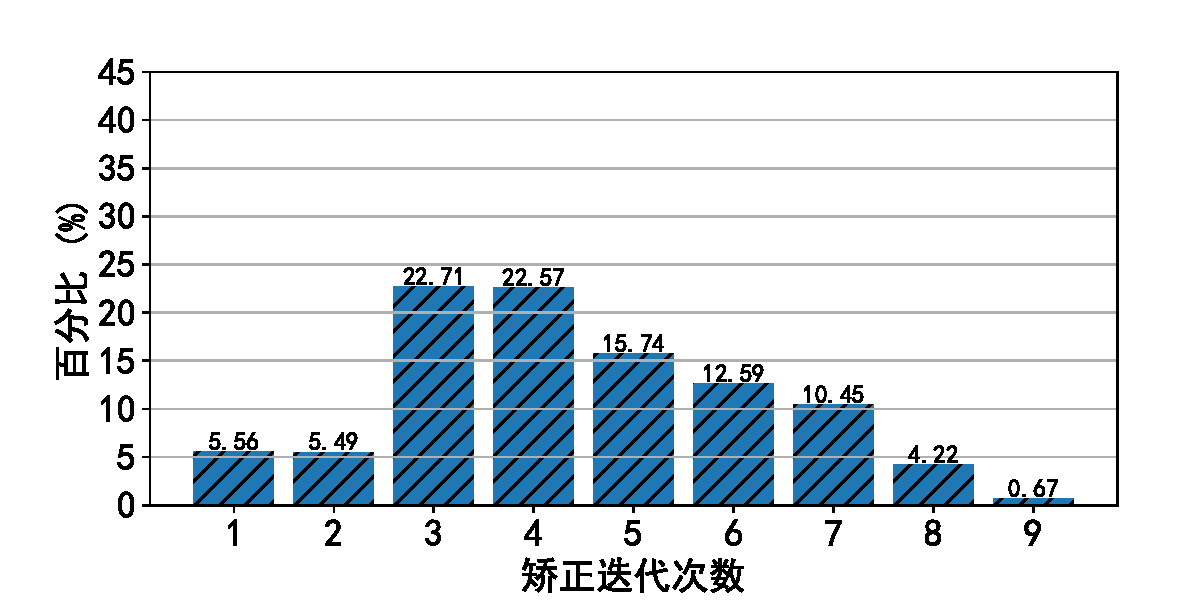
\includegraphics[width=0.95\linewidth]{fig/fix/distribution.pdf}}
\caption{成功消除不稳定因素的配置数量分布}
\label{fig:fix_distribution}
\end{figure}

\end{itemize}


\subsection{时间消耗}
实验通过分别计算训练智能体和缓解不稳定状态的时间成本来评估系统的效率。

\begin{itemize}
    \item \textbf{智能体训练.}
在智能体的训练过程中,\nyctea 消耗了 $22$ 小时从所有的不正确配置的训练集中学习修复经验。 
由于模型训练成本是一次性成本,因此 $22$ 小时是可以接受的时间成本。

    \item \textbf{状态矫正.}
实验单独评估了生成每个配置的时间消耗。
实验在 \tool{Ardupilot} 和 \tool{PX4} 中各自运智能体 500 次来创建配置。
由于模型的网络架构一直,因此两种智能体生成一种配置平均花费为 0.12ms。

\end{itemize}

    

\subsection{研究比较}
此节将 \nyctea 与其他最先进的方法(表~\ref{tab:cmp_other}) 一起讨论,这些方法也可以识别或修复影响无人机稳定性的问题。
用于解决无人机系统不稳定性的方法从两个角度解决该问题:内部错误处理和外部攻击。
内部错误处理是指由于配置错误、控制逻辑问题或安全逻辑问题等事件导致无人机不稳定的问题。
外部攻击是指由恶意活动引起的问题,例如配置攻击、传感器攻击或测量欺骗。
而用于解决无人机系统不稳定性的方法可分为三类:补丁、限制和冗余。
补丁方法涉及使用新补丁更新代码、配置、动态调整这几种方法以减少不稳定性。
限制方法利用严格的限制条件来最大程度地减少不稳定发生的可能性。
冗余方法采用额外软模块,当无人机变得不稳定时,这些模块会成为冗余控制,接管当前飞行控制系统以确保系统继续有效运行。

\begin{table*}[tb]
\caption{与最先进研究的比较}
\label{tab:cmp_other}
\centering
\begin{threeparttable}
\begin{tabular}{c|ccccccc}
        \toprule[1.5pt]
    
           & {问题源} & {修复手段} & {\makecell*[c]{在线 \\ 支持}} & {\makecell*[c]{需要 \\ 预训练}}  &  {\makecell*[c]{彻底 \\ 修复}} &{\makecell*[c]{无代码 \\ 插入} }  & {\makecell*[c]{无任务 \\ 限制} } \\
        \midrule[0.8pt]
        
          \nyctea & 内与外 & 补丁 & \ding{51} & \ding{51}  & \ding{55} & \ding{51} &  \ding{51}  \\

          \tool{LGDFuzzr}~\cite{han2022control} & 内与外 & 限制 & \ding{55} & \ding{51} & \ding{55}  & \ding{51} &  \ding{55} \\

          \tool{RVFuzzr}~\cite{rvfuzzer} & 内与外 & 限制 & \ding{55} & \ding{51} & \ding{55} & \ding{51} &  \ding{55}  \\

          \tool{DisPatch}~\cite{kim2022reverse} & 内部 & 补丁 & \ding{55} & \ding{55} &  \ding{51} & \ding{55} & \ding{51} \\

          \tool{Avis}~\cite{taylor2021avis} & 内部 & 补丁 & \ding{55} & \ding{55} & \ding{51} & \ding{55} &  \ding{51}  \\
            
          \tool{PID-Piper}~\cite{dash2021pid} & 外部 & 冗余 & \ding{51} & \ding{51} & \ding{55} & \ding{55} &  \ding{51}  \\

          \tool{Soft-sensors}~\cite{choi2020software} & 外部 & 冗余 & \ding{51} & \ding{51} & \ding{55} & \ding{55} &  \ding{51}  \\

      
        \bottomrule[1.5pt]
\end{tabular}
% \begin{tablenotes}
% \footnotesize
% \item[*] {Int} is internal. 
% {Exter} is exterinal.
% \end{tablenotes}
\end{threeparttable}
\end{table*}

\tool{LGDFuzzer}和\tool{RVFuzzer}采用模糊测试方法来搜索潜在问题并构建对无人机的限制,从而降低控制逻辑问题导致不稳定的可能性。
这些方法可以抵抗内部和外部问题,但这并不适合线上出现的未预料的意外情况。
此外,他们采用的限制手段降低了无人机适应不同任务的能力,这可能无法满足某些用户的要求。
\tool{DisPatch}和\tool{Avis}应用静态分析来检测代码中的内部逻辑问题并创建补丁以提高无人机稳定性。
对于部分代码逻辑引起的错误,他们可以进行完整的修复,但是静态分析的覆盖范围使他们无法覆盖所有情况。
而且这些补丁不具有适应性,这意味着不同的控制程序可能需要独特的补丁。
\tool{PID-Piper}和\tool{Soft-sensors}构造一个软件算法模块来为飞行控制器实现一致的冗余功能。
当检测到异常时,它们会切换到冗余模块作为控制器。
但这些冗余模块需要对原有控制程序进行代码修改,且针对特定车型,适应性较差,不能普遍适用于各种车辆。
另外,如果不稳定是由内部逻辑问题引起的,那么这种冗余模型就无能为力。
与其他方法相比,\nyctea 可以通过其本机重新配置机制动态处理内部和外部问题,而不需要任何代码修改。 
与冗余不同,\nyctea 不需要更改原始代码。
与限制不同的是,\nyctea 不会影响无人机的环境适应性。 
此外,与其他修补方法不同,\nyctea 支持在线修补,可以实时动态矫正无人机。


\subsection{案例研究}
实验进行了两次可比较的飞行执行,以演示系统如何消除不稳定。

实验用\tool{Ardupilot}实现了一架无人机,在模拟器\tool{APM}中执行飞行任务\tool{AVC2013}。
实验首先在没有集成\nyctea 的情况下执行飞行任务,如图~\ref{subfig:fix_thurst_raw}所示。
无人机使用默认配置起飞。
在时间戳 104(10.4 秒)之后,实验上传了一个可能导致推力损失警告的不正确。
随后无人机开始晃动,偏差逐渐加大。
31.2秒时,飞行任务终止,无人机发出推力损失警告。
在第二次执行中,实验将 \nyctea 应用于\tool{Ardupilot} 并复制了第一个实验设定。
图~\ref{subfig:fix_repair}展示了Roll、Pitch、Yaw的详细状态变化。
图中的结果清楚地表明,\ nyctea 在18.9秒识别出不稳定,并启动状态整流模块进行整流。
然后 \nyctea  在 18.9秒、23秒、27.1秒、38.3秒 和 47.8秒 上传了 5 个配置。
虽然初始配置并没有显着缓解不稳定的情况,后续的四个配置逐渐将偏差缩小到较小范围。
第五次校正上传完成后,观测到的偏差逐渐减小,无人机的状态(即横滚、俯仰、偏航)趋于稳定。
 
\begin{figure*}[htb]
\centering
\begin{minipage}{0.49\linewidth}
    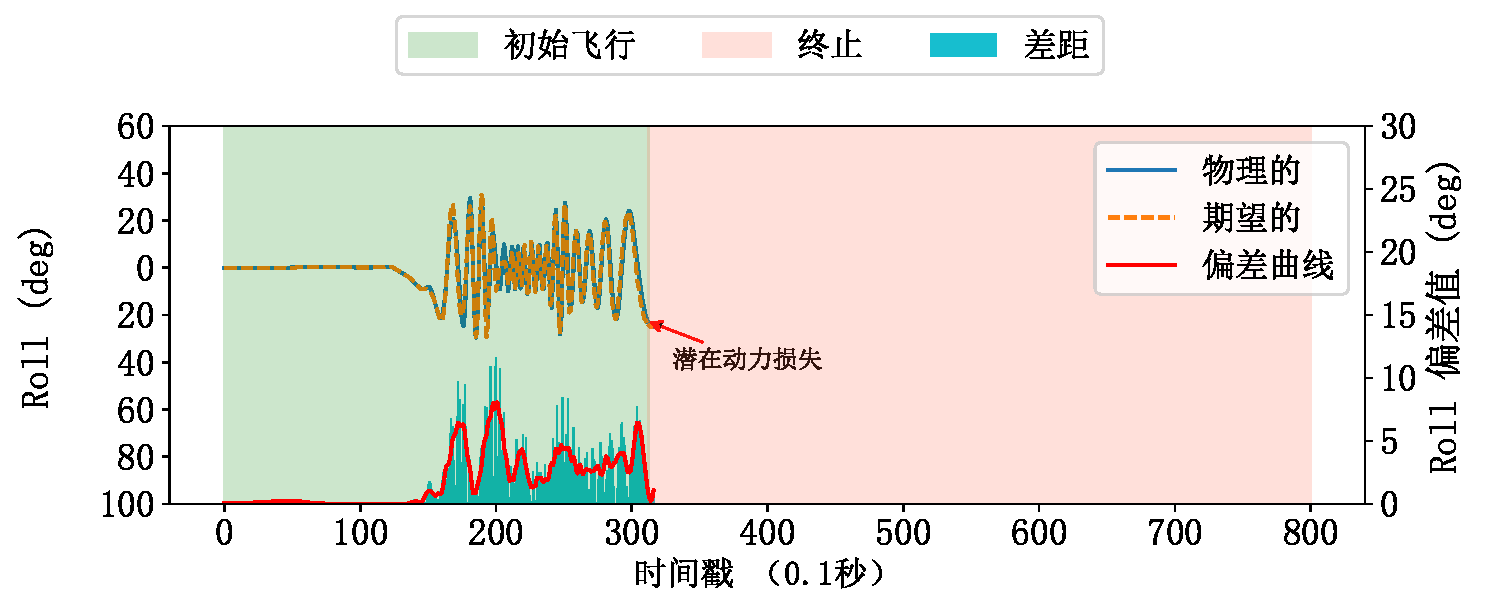
\includegraphics[width=\linewidth]{fig/fix/fix/raw_thrust_roll.pdf}\quad
    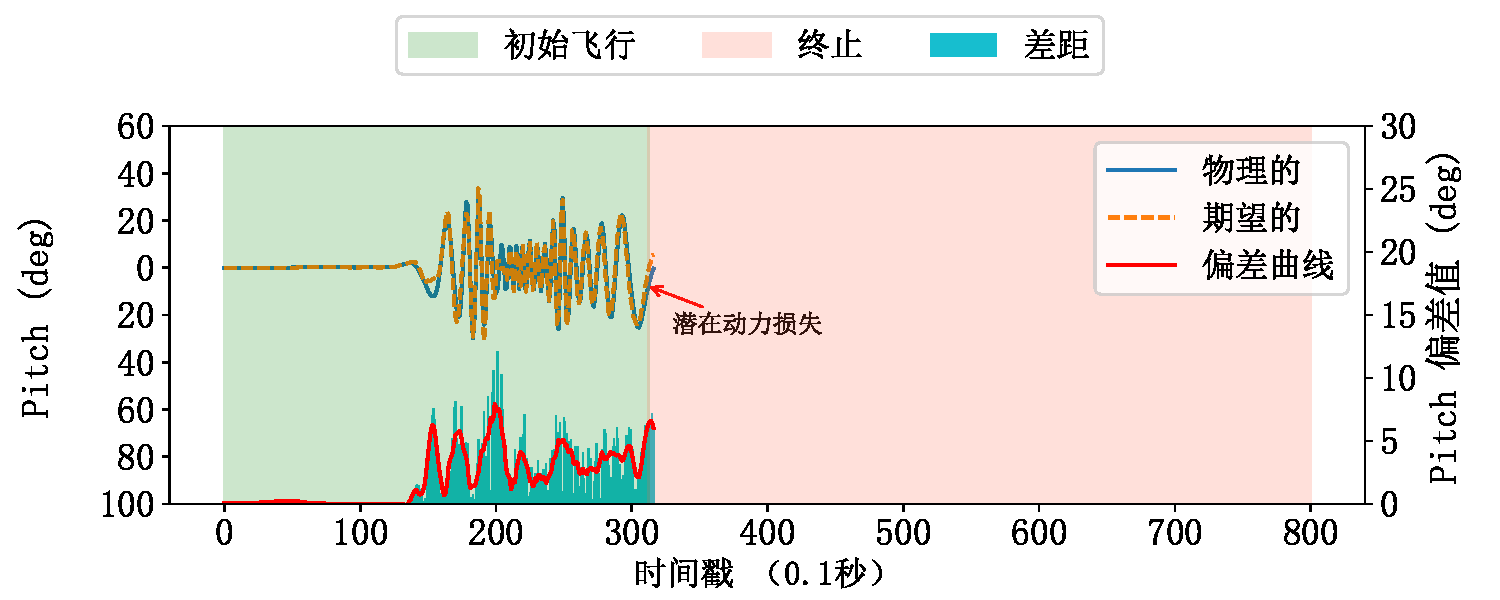
\includegraphics[width=\linewidth]{fig/fix/fix/raw_thrust_pitch.pdf}\quad
    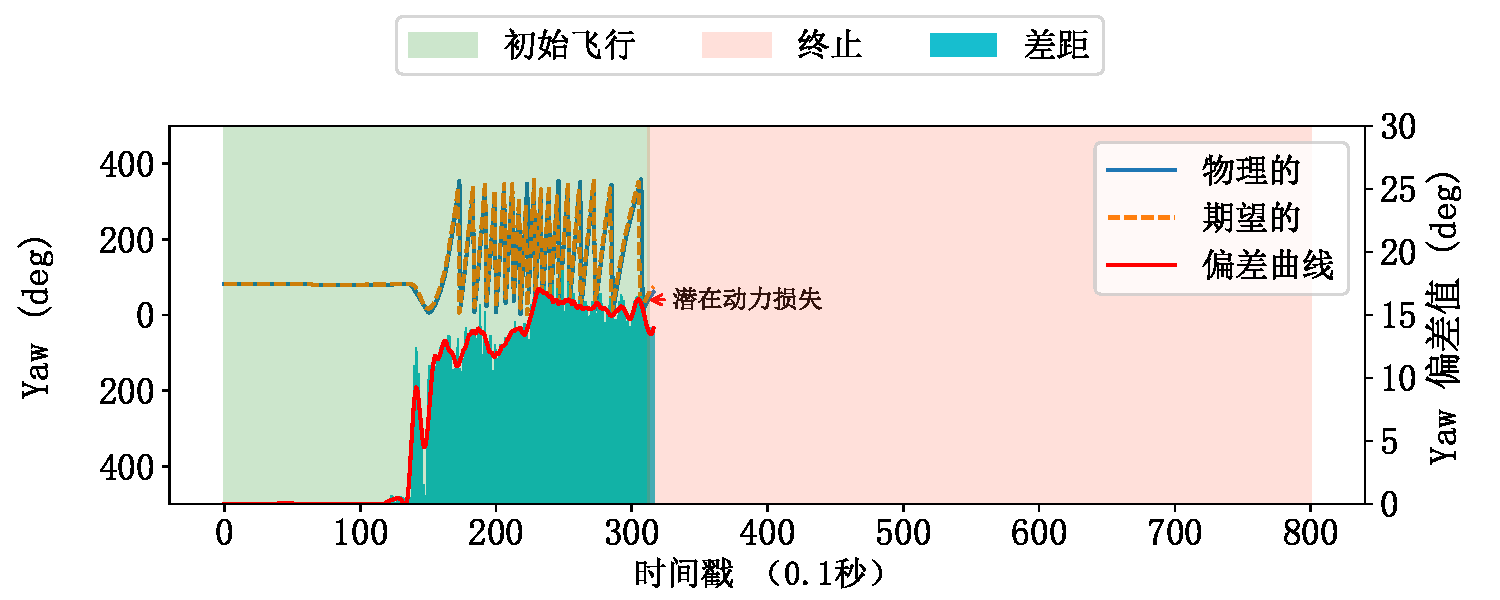
\includegraphics[width=\linewidth]{fig/fix/fix/raw_thrust_yaw.pdf}
    \caption{未装备\nyctea 无人机的状态}
    \label{subfig:fix_thurst_raw}
\end{minipage}
\begin{minipage}{0.49\linewidth}
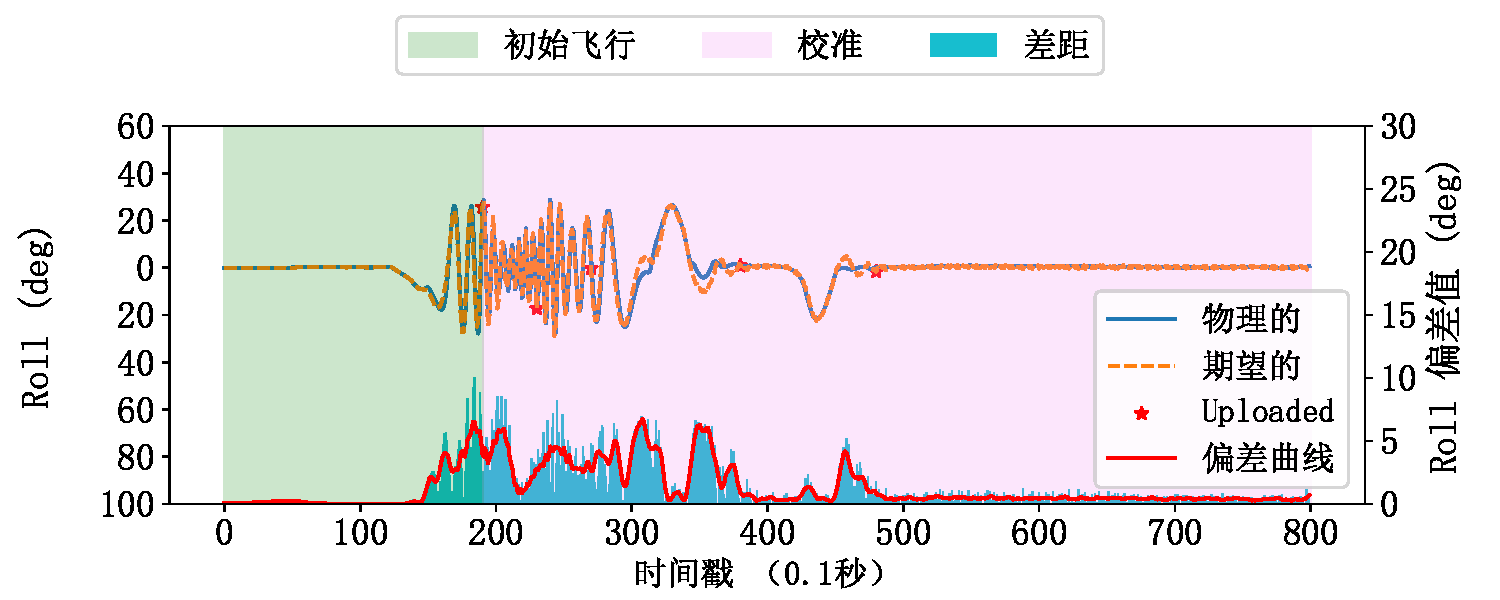
\includegraphics[width=\linewidth]{fig/fix/fix/fix_thrust_roll.pdf}\quad
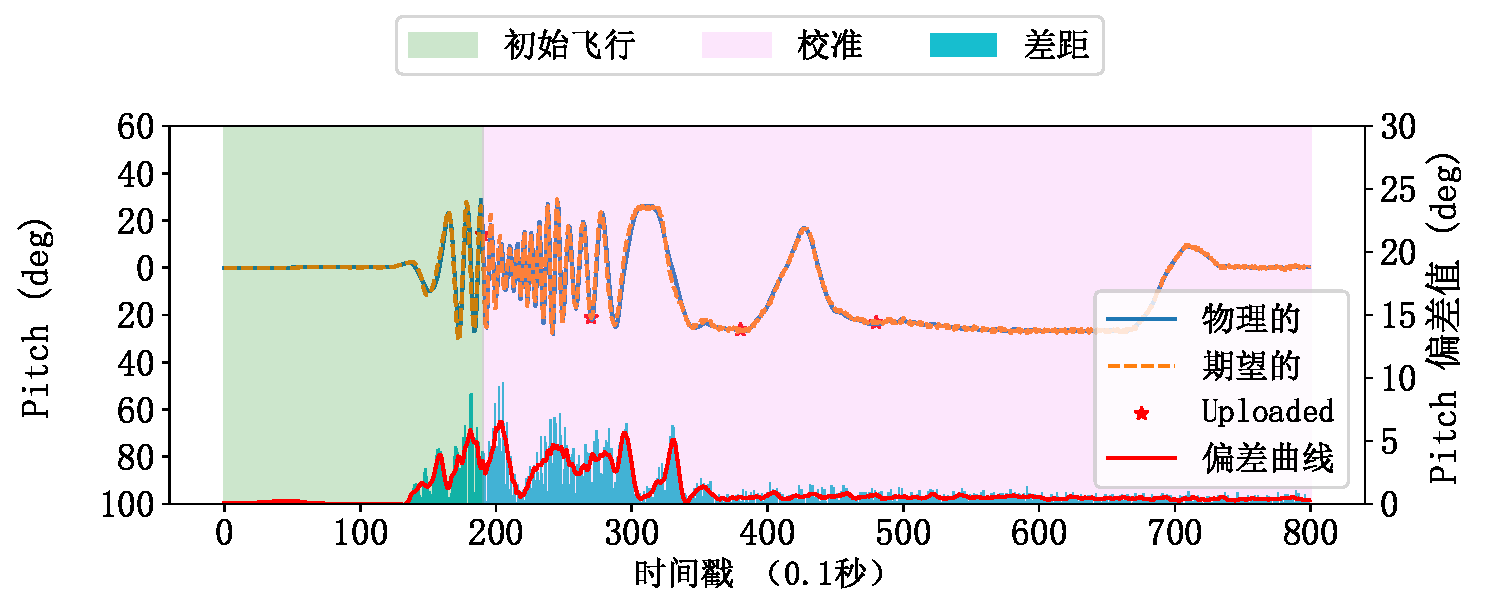
\includegraphics[width=\linewidth]{fig/fix/fix/fix_thrust_pitch.pdf}\quad
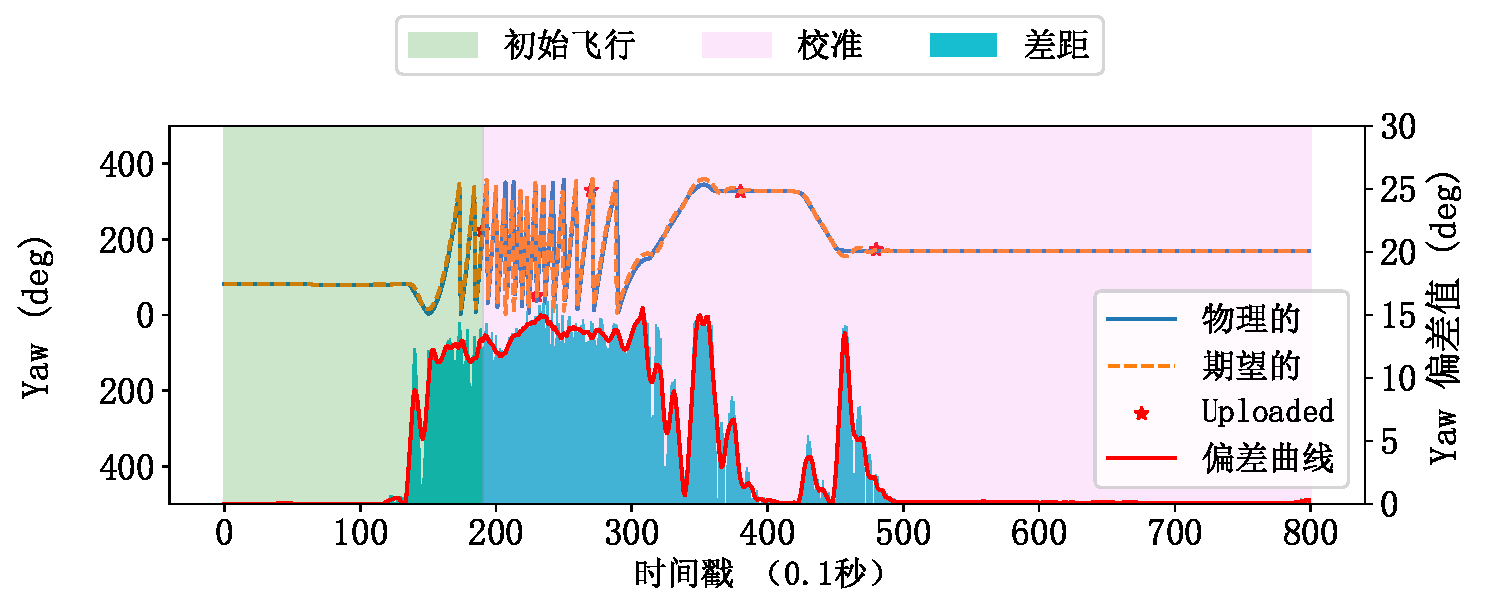
\includegraphics[width=\linewidth]{fig/fix/fix/fix_thrust_yaw.pdf}
\caption{未装备\nyctea 无人机的状态}
\label{subfig:fix_repair}
\end{minipage}


\end{figure*}

在第二个现实样例中,实验使用真实的无人机(\tool{CUAV ZD550})来测试\nyctea 的真实表现。 
整个不正确配置造成的相应的状态变化可以在图~\ref{fig:fix_deviation_change_real}中观察到。
在飞行过程中,物理状态在接受了配置后逐渐变得不稳定,并在到达任务航路点后开始振动。
\nyctea 识别出不稳定的物理状态并启动了第一次矫正(第一个 \emph{uploaded} 标记)。
虽然矫正减少了偏差,但并没有完全缓解问题。
\nyctea 生成了另一次矫正(第二个 \emph{uploaded} 标记),使无人机能够重新获得稳定飞行并成功完成任务。
总的来说,\nyctea 系统可以有效地识别和矫正现实飞行场景中的不稳定问题。


\begin{figure}[htb]
\centering{
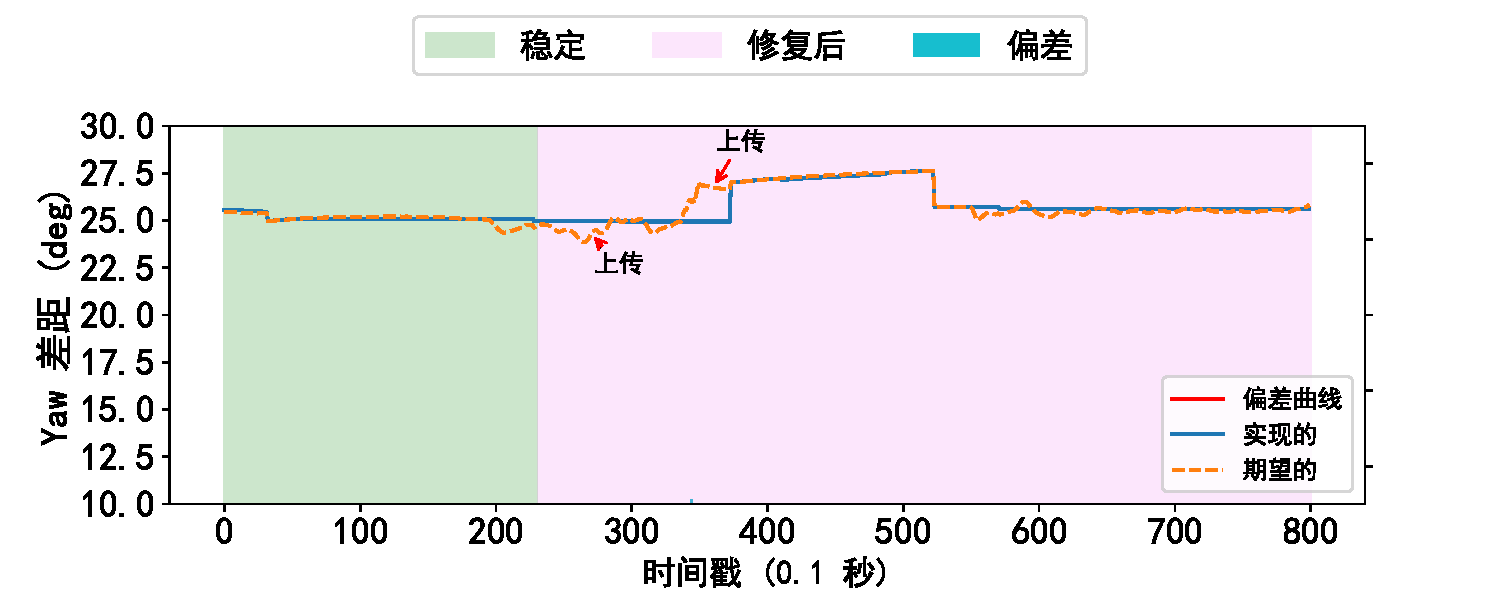
\includegraphics[width=0.98\linewidth]{fig/fix/fix/real_repair.pdf}}
\caption{真实无人机的 \nyctea 校正示例}
\label{fig:fix_deviation_change_real}
\end{figure}


\section{本章小结}
当无人机受到配置攻击或者传感器攻击时,可能会出现坠毁或者其他严重的事故。
本章节提出了一种在线修复系统--\nyctea ,它能实时检测并矫正由攻击或用户错误引起的不稳定物理状态,以防止无人机飞行过程中出现最糟糕的情况。
该系统通过计算已实现状态与期望状态之间的段偏差值来有效识别不稳定状态,并利用强化学习为无人机生成适当的配置。
实验测试了证明了\nyctea 的效率和修复成功率,结果表明其修复性能良好。

\chapter{总结与展望}
\section{本文工作总结}
本工作从三个角度探讨了无人机安全性和可靠性的增强方法进行了讨论。

首先,文章从无人机系统的安全检查机制入手,用来解决飞行过程中由\emph{不足事件}和\emph{过度事件}引起的模块检查错误。
\deccheck 模块使用状态不变量和机器学习分类方法来解决上述事件。
\deccheck 建立了收集各种事件数据的环境,利用神经网络来提取飞行状态的不变量。
\deccheck 应用该不变因素为每个事件创建相应的不变差异特征,并训练一个\tool{CNN}模型来检测它们。
本文在模拟和真实的无人机上评估了该系统。
不变量提供了超过98\%的预测精度,每个类别的分类器的F1分数都超过90\%。
与原来的安全检查相比,\deccheck 增强了对特殊物理事件的检测能力。

针对无人机系统控制本身,本文通过\icsearcher 发现了\emph{范围规范错误},该错误是由合法用户或者攻击者触发的一种系统逻辑问题。
最严重的情况会导致飞行不稳定,中断无人机的正常飞行任务。
同时,为了应对这种问题,文章通过设计\icsearcher 模块这样一个基于模糊测试的系统来效地搜索潜在的不正确参数配置。
\icsearcher 使用启发式搜索的手段进行配置搜素,同时通过使用机器学习的预测模型来辅助模糊搜索过程。
最终,通过多目标优化,\icsearcher 实现了一种简单的建议范围的生成方法,初步得解决了这种配置漏洞带来的安全问题,降低了无人机飞行过程中出现不稳定状态的概率。
本章将该工具与其他先进研究进行比较,表明了\icsearcher 自身系统的优越性。

在初步讨论了\emph{范围规范错误}所带来的问题后,文章针对范围限制的这种补救形式的不足,进一步的提出了在线修复的思路。
\nyctea 可以在无人机飞行过程中高效地检测出由\emph{范围规范错误}引起的不稳定飞行状态,同时提供更加合适的整改方案。
再确定了无人机正处于危机时刻的时候,\nyctea 使用预先训练的强化学习智能体来进行迭代矫正,指导无人机稳定飞行。
本文通过实验测试进一步论证了\nyctea 模块的修复效率和成功率。


\section{研究展望}
本文探讨了三种无人机系统安全与可靠性增强机制,后续计划研究如下:
\begin{enumerate}
    \item 进行适配迁移,将\deccheck 应用于更多无人机操作系统当中。同时引入自动化的方法,更加精准的采集无任务发生安全事件后的数据变化模式,提高系统在对事件进行识别时的准确性,降低不同类别之间数据分类的干扰,降低误报率。

    \item 由于Range Specification Bugs是通过Fuzzing确定的,目前尚不清楚其根本性原理。
    计划采用动态静态相结合的方法,精准定位设计的缺陷之处,在无人机汇报安全问题的同时,精准快速定位参数问题的根本所在,以最小的修改代价稳定无人机的飞行姿态,确保无人机的飞行任务顺利完成。
    
\end{enumerate}

\backmatter

\end{document}
